% **************************************************************************************************************
% A Classic Thesis Style
% An Homage to The Elements of Typographic Style
%
% Copyright (C) 2017 André Miede and Ivo Pletikosić
%
% If you like the style then I would appreciate a postcard. My address
% can be found in the file ClassicThesis.pdf. A collection of the
% postcards I received so far is available online at
% http://postcards.miede.de
%
% License:
% This program is free software; you can redistribute it and/or modify
% it under the terms of the GNU General Public License as published by
% the Free Software Foundation; either version 2 of the License, or
% (at your option) any later version.
%
% This program is distributed in the hope that it will be useful,
% but WITHOUT ANY WARRANTY; without even the implied warranty of
% MERCHANTABILITY or FITNESS FOR A PARTICULAR PURPOSE.  See the
% GNU General Public License for more details.
%
% You should have received a copy of the GNU General Public License
% along with this program; see the file COPYING.  If not, write to
% the Free Software Foundation, Inc., 59 Temple Place - Suite 330,
% Boston, MA 02111-1307, USA.
%
% PLEASE SEE ALSO THE AUTHORS' NOTE REGARDING THIS LICENSE
% IN THE DOCUMENTATION (ClassicThesis.pdf --> Chapter 1 / Chapter01.tex)
% **************************************************************************************************************
\RequirePackage{silence} % :-\
    \WarningFilter{scrreprt}{Usage of package `titlesec'}
    \WarningFilter{titlesec}{Non standard sectioning command detected}
\documentclass[ twoside,openright,titlepage,numbers=noenddot,headinclude,%1headlines,% letterpaper a4paper
                footinclude=true,cleardoublepage=empty,abstractoff, % <--- obsolete, remove (todo)
                BCOR=5mm,paper=a4,fontsize=11pt,%11pt,a4paper,%
                american,%
                ]{scrreprt}

%********************************************************************
% Note: Make all your adjustments in here
%*******************************************************
% ****************************************************************************************************
% classicthesis-config.tex
% formerly known as loadpackages.sty, classicthesis-ldpkg.sty, and classicthesis-preamble.sty
% Use it at the beginning of your ClassicThesis.tex, or as a LaTeX Preamble
% in your ClassicThesis.{tex,lyx} with % ****************************************************************************************************
% classicthesis-config.tex
% formerly known as loadpackages.sty, classicthesis-ldpkg.sty, and classicthesis-preamble.sty
% Use it at the beginning of your ClassicThesis.tex, or as a LaTeX Preamble
% in your ClassicThesis.{tex,lyx} with % ****************************************************************************************************
% classicthesis-config.tex
% formerly known as loadpackages.sty, classicthesis-ldpkg.sty, and classicthesis-preamble.sty
% Use it at the beginning of your ClassicThesis.tex, or as a LaTeX Preamble
% in your ClassicThesis.{tex,lyx} with \input{classicthesis-config}
% ****************************************************************************************************
% If you like the classicthesis, then I would appreciate a postcard.
% My address can be found in the file ClassicThesis.pdf. A collection
% of the postcards I received so far is available online at
% http://postcards.miede.de
% ****************************************************************************************************


% ****************************************************************************************************
% 0. Set the encoding of your files. UTF-8 is the only sensible encoding nowadays. If you can't read
% äöüßáéçèê∂åëæƒÏ€ then change the encoding setting in your editor, not the line below. If your editor
% does not support utf8 use another editor!
% ****************************************************************************************************
\PassOptionsToPackage{utf8}{inputenc}
  \usepackage{inputenc}

% ****************************************************************************************************
% 1. Configure classicthesis for your needs here, e.g., remove "drafting" below
% in order to deactivate the time-stamp on the pages
% (see ClassicThesis.pdf for more information):
% ****************************************************************************************************
\PassOptionsToPackage{
  drafting=false,    % print version information on the bottom of the pages
  tocaligned=false, % the left column of the toc will be aligned (no indentation)
  dottedtoc=false,  % page numbers in ToC flushed right
  parts=true,       % use part division
  eulerchapternumbers=true, % use AMS Euler for chapter font (otherwise Palatino)
  linedheaders=false,       % chaper headers will have line above and beneath
  floatperchapter=true,     % numbering per chapter for all floats (i.e., Figure 1.1)
  listings=true,    % load listings package and setup LoL
  subfig=true,      % setup for preloaded subfig package
  eulermath=false,  % use awesome Euler fonts for mathematical formulae (only with pdfLaTeX)
  beramono=true,    % toggle a nice monospaced font (w/ bold)
  minionpro=false   % setup for minion pro font; use minion pro small caps as well (only with pdfLaTeX)
}{classicthesis}


% ****************************************************************************************************
% 2. Personal data and user ad-hoc commands
% ****************************************************************************************************
\newcommand{\myTitle}{Gestor de Trending Topics y Noticias\xspace}
\newcommand{\mySubtitle}{Estudio y Visualización de Trends de Twitter\xspace}
\newcommand{\myDegree}{Grado en Ingeniería Informática\xspace}
\newcommand{\myName}{Nikita Stetskiy Stetskiy (alumno)\xspace}
\newcommand{\myProf}{Juan Francisco Huete Guadix (tutor)\xspace}
\newcommand{\myOtherProf}{Carlos Alberto Cruz Corona (cotutor)\xspace}
%\newcommand{\mySupervisor}{Put name here\xspace}
\newcommand{\myFaculty}{Escuela Técnica Superior de Ingenierías Informática y de Telecomunicación\xspace}
\newcommand{\myDepartment}{Departamento de de Ciencias de la Computación de Inteligencia Artificial\xspace}
\newcommand{\myUni}{E.T.S. de Ingenierías Informática y de Telecomunicación\xspace}
\newcommand{\myLocation}{Granada\xspace}
\newcommand{\myTime}{\today\xspace}
\newcommand{\myVersion}{Version 0.1}

% ********************************************************************
% Setup, finetuning, and useful commands
% ********************************************************************
\newcounter{dummy} % necessary for correct hyperlinks (to index, bib, etc.)
\newlength{\abcd} % for ab..z string length calculation
\providecommand{\mLyX}{L\kern-.1667em\lower.25em\hbox{Y}\kern-.125emX\@}
\newcommand{\ie}{i.\,e.}
\newcommand{\Ie}{I.\,e.}
\newcommand{\eg}{e.\,g.}
\newcommand{\Eg}{E.\,g.}
% ****************************************************************************************************


% ****************************************************************************************************
% 3. Loading some handy packages
% ****************************************************************************************************
\usepackage{varwidth}
\usepackage[boxruled]{algorithm2e}
\SetKwProg{Fn}{Function}{}{end}
\SetKwProg{Proc}{Procedure}{}{end}
\usepackage{fixltx2e}
\usepackage{float}
% ********************************************************************
% Packages with options that might require adjustments
% ********************************************************************
%\PassOptionsToPackage{ngerman,american}{babel}   % change this to your language(s), main language last
% Spanish languages need extra options in order to work with this template
\PassOptionsToPackage{spanish,es-lcroman}{babel}
    \usepackage[spanish]{babel}

\usepackage{csquotes}
\PassOptionsToPackage{%
  %backend=biber,bibencoding=utf8, %instead of bibtex
  backend=bibtex8,bibencoding=ascii,%
  language=spanish,%
  style=numeric-comp,%
  %style=authoryear-comp, % Author 1999, 2010
  %bibstyle=authoryear,dashed=false, % dashed: substitute rep. author with ---
  sorting=none, % name, year, title
  maxbibnames=10, % default: 3, et al.
  %backref=true,%
  natbib=true % natbib compatibility mode (\citep and \citet still work)
}{biblatex}
    \usepackage{biblatex}

\PassOptionsToPackage{fleqn}{amsmath}       % math environments and more by the AMS
  \usepackage{amsmath}

% ********************************************************************
% General useful packages
% ********************************************************************
\PassOptionsToPackage{T1}{fontenc} % T2A for cyrillics
  \usepackage{fontenc}
\usepackage{textcomp} % fix warning with missing font shapes
\usepackage{scrhack} % fix warnings when using KOMA with listings package
\usepackage{xspace} % to get the spacing after macros right
\usepackage{mparhack} % get marginpar right
%\usepackage{fixltx2e} % fixes some LaTeX stuff --> since 2015 in the LaTeX kernel (see below)
% \usepackage[latest]{latexrelease} % emulate newer kernel version if older is detected
\PassOptionsToPackage{printonlyused,smaller}{acronym}
  \usepackage{acronym} % nice macros for handling all acronyms in the thesis
  %\renewcommand{\bflabel}[1]{{#1}\hfill} % fix the list of acronyms --> no longer working
  %\renewcommand*{\acsfont}[1]{\textsc{#1}}
  %\renewcommand*{\aclabelfont}[1]{\acsfont{#1}}
  %\def\bflabel#1{{#1\hfill}}
  \def\bflabel#1{{\acsfont{#1}\hfill}}
  \def\aclabelfont#1{\acsfont{#1}}
% ****************************************************************************************************
%\usepackage{pgfplots} % External TikZ/PGF support (thanks to Andreas Nautsch)
%\usetikzlibrary{external}
%\tikzexternalize[mode=list and make, prefix=ext-tikz/]
% ****************************************************************************************************


% ****************************************************************************************************
% 4. Setup floats: tables, (sub)figures, and captions
% ****************************************************************************************************
\usepackage{tabularx} % better tables
  \setlength{\extrarowheight}{3pt} % increase table row height
\newcommand{\tableheadline}[1]{\multicolumn{1}{c}{\spacedlowsmallcaps{#1}}}
\newcommand{\myfloatalign}{\centering} % to be used with each float for alignment
\usepackage{caption}
% Thanks to cgnieder and Claus Lahiri
% http://tex.stackexchange.com/questions/69349/spacedlowsmallcaps-in-caption-label
% [REMOVED DUE TO OTHER PROBLEMS, SEE ISSUE #82]
%\DeclareCaptionLabelFormat{smallcaps}{\bothIfFirst{#1}{~}\MakeTextLowercase{\textsc{#2}}}
%\captionsetup{font=small,labelformat=smallcaps} % format=hang,
\captionsetup{font=small} % format=hang,
\usepackage{subfig}
% ****************************************************************************************************


% ****************************************************************************************************
% 5. Setup code listings
% ****************************************************************************************************
\usepackage{listings}
%\lstset{emph={trueIndex,root},emphstyle=\color{BlueViolet}}%\underbar} % for special keywords
\lstset{language=[LaTeX]Tex,%C++,
  morekeywords={PassOptionsToPackage,selectlanguage},
  keywordstyle=\color{RoyalBlue},%\bfseries,
  basicstyle=\small\ttfamily,
  %identifierstyle=\color{NavyBlue},
  commentstyle=\color{Green}\ttfamily,
  stringstyle=\rmfamily,
  numbers=none,%left,%
  numberstyle=\scriptsize,%\tiny
  stepnumber=5,
  numbersep=8pt,
  showstringspaces=false,
  breaklines=true,
  %frameround=ftff,
  %frame=single,
  belowcaptionskip=.75\baselineskip
  %frame=L
}
% ****************************************************************************************************


% ****************************************************************************************************
% 6. PDFLaTeX, hyperreferences, and citation backreferences
% ****************************************************************************************************
% ********************************************************************
% Using PDFLaTeX
% ********************************************************************
\PassOptionsToPackage{hyperfootnotes=false,pdfpagelabels}{hyperref}
  \usepackage{hyperref}  % backref linktocpage pagebackref
%\ifpdf
%\pdfcompresslevel=9
%\pdfadjustspacing=1
%\fi
%\PassOptionsToPackage{pdftex}{graphicx} %%%IVO: driver will be chosen automatically
  \usepackage{graphicx}


% ********************************************************************
% Hyperreferences
% ********************************************************************
\hypersetup{%
  %draft, % hyperref's draft mode, for printing see below
  colorlinks=true, linktocpage=true, pdfstartpage=3, pdfstartview=FitV,%
  % uncomment the following line if you want to have black links (e.g., for printing)
  %colorlinks=false, linktocpage=false, pdfstartpage=3, pdfstartview=FitV, pdfborder={0 0 0},%
  breaklinks=true, pdfpagemode=UseNone, pageanchor=true, pdfpagemode=UseOutlines,%
  plainpages=false, bookmarksnumbered, bookmarksopen=true, bookmarksopenlevel=1,%
  hypertexnames=true, pdfhighlight=/O,%nesting=true,%frenchlinks,%
  urlcolor=blue, linkcolor=RoyalBlue, citecolor=webgreen, %pagecolor=RoyalBlue,%
  %urlcolor=Black, linkcolor=Black, citecolor=Black, %pagecolor=Black,%
  pdftitle={\myTitle},%
  pdfauthor={\textcopyright\ \myName, \myUni, \myFaculty},%
  pdfsubject={},%
  pdfkeywords={},%
  pdfcreator={pdfLaTeX},%
  pdfproducer={LaTeX with hyperref and classicthesis}%
}

% ********************************************************************
% Setup autoreferences
% ********************************************************************
% There are some issues regarding autorefnames
% http://www.ureader.de/msg/136221647.aspx
% http://www.tex.ac.uk/cgi-bin/texfaq2html?label=latexwords
% you have to redefine the makros for the
% language you use, e.g., american, ngerman
% (as chosen when loading babel/AtBeginDocument)
% ********************************************************************
\makeatletter
\@ifpackageloaded{babel}%
  {%
    \addto\extrasamerican{%
      \renewcommand*{\figureautorefname}{Figure}%
      \renewcommand*{\tableautorefname}{Table}%
      \renewcommand*{\partautorefname}{Part}%
      \renewcommand*{\chapterautorefname}{Chapter}%
      \renewcommand*{\sectionautorefname}{Section}%
      \renewcommand*{\subsectionautorefname}{Section}%
      \renewcommand*{\subsubsectionautorefname}{Section}%
    }%
    \addto\extrasngerman{%
      \renewcommand*{\paragraphautorefname}{Absatz}%
      \renewcommand*{\subparagraphautorefname}{Unterabsatz}%
      \renewcommand*{\footnoteautorefname}{Fu\"snote}%
      \renewcommand*{\FancyVerbLineautorefname}{Zeile}%
      \renewcommand*{\theoremautorefname}{Theorem}%
      \renewcommand*{\appendixautorefname}{Anhang}%
      \renewcommand*{\equationautorefname}{Gleichung}%
      \renewcommand*{\itemautorefname}{Punkt}%
    }%
      % Fix to getting autorefs for subfigures right (thanks to Belinda Vogt for changing the definition)
      \providecommand{\subfigureautorefname}{\figureautorefname}%
    }{\relax}
\makeatother


% ****************************************************************************************************
% 7. Last calls before the bar closes
% ****************************************************************************************************
% ********************************************************************
% Development Stuff
% ********************************************************************
\listfiles
%\PassOptionsToPackage{l2tabu,orthodox,abort}{nag}
%  \usepackage{nag}
%\PassOptionsToPackage{warning, all}{onlyamsmath}
%  \usepackage{onlyamsmath}

% ********************************************************************
% Last, but not least...
% ********************************************************************
\usepackage[dottedtoc]{classicthesis}
% ****************************************************************************************************


% ****************************************************************************************************
% 8. Further adjustments (experimental)
% ****************************************************************************************************
% ********************************************************************
% Changing the text area
% ********************************************************************
%\areaset[current]{312pt}{761pt} % 686 (factor 2.2) + 33 head + 42 head \the\footskip
%\setlength{\marginparwidth}{7em}%
%\setlength{\marginparsep}{2em}%

% ********************************************************************
% Using different fonts
% ********************************************************************
%\usepackage[oldstylenums]{kpfonts} % oldstyle notextcomp
%\usepackage[osf]{libertine}
%\usepackage[light,condensed,math]{iwona}
%\renewcommand{\sfdefault}{iwona}
%\usepackage{lmodern} % <-- no osf support :-(
%\usepackage{cfr-lm} %
%\usepackage[urw-garamond]{mathdesign} <-- no osf support :-(
%\usepackage[default,osfigures]{opensans} % scale=0.95
%\usepackage[sfdefault]{FiraSans}
% ********************************************************************
% \usepackage[largesc,osf]{newpxtext}
% Used to fix these:
% https://bitbucket.org/amiede/classicthesis/issues/139/italics-in-pallatino-capitals-chapter
% https://bitbucket.org/amiede/classicthesis/issues/45/problema-testatine-su-classicthesis-style
% ********************************************************************
%\linespread{1.05} % a bit more for Palatino
% ****************************************************************************************************
% ****************************************************************************************************
% If you like the classicthesis, then I would appreciate a postcard.
% My address can be found in the file ClassicThesis.pdf. A collection
% of the postcards I received so far is available online at
% http://postcards.miede.de
% ****************************************************************************************************


% ****************************************************************************************************
% 0. Set the encoding of your files. UTF-8 is the only sensible encoding nowadays. If you can't read
% äöüßáéçèê∂åëæƒÏ€ then change the encoding setting in your editor, not the line below. If your editor
% does not support utf8 use another editor!
% ****************************************************************************************************
\PassOptionsToPackage{utf8}{inputenc}
  \usepackage{inputenc}

% ****************************************************************************************************
% 1. Configure classicthesis for your needs here, e.g., remove "drafting" below
% in order to deactivate the time-stamp on the pages
% (see ClassicThesis.pdf for more information):
% ****************************************************************************************************
\PassOptionsToPackage{
  drafting=false,    % print version information on the bottom of the pages
  tocaligned=false, % the left column of the toc will be aligned (no indentation)
  dottedtoc=false,  % page numbers in ToC flushed right
  parts=true,       % use part division
  eulerchapternumbers=true, % use AMS Euler for chapter font (otherwise Palatino)
  linedheaders=false,       % chaper headers will have line above and beneath
  floatperchapter=true,     % numbering per chapter for all floats (i.e., Figure 1.1)
  listings=true,    % load listings package and setup LoL
  subfig=true,      % setup for preloaded subfig package
  eulermath=false,  % use awesome Euler fonts for mathematical formulae (only with pdfLaTeX)
  beramono=true,    % toggle a nice monospaced font (w/ bold)
  minionpro=false   % setup for minion pro font; use minion pro small caps as well (only with pdfLaTeX)
}{classicthesis}


% ****************************************************************************************************
% 2. Personal data and user ad-hoc commands
% ****************************************************************************************************
\newcommand{\myTitle}{Gestor de Trending Topics y Noticias\xspace}
\newcommand{\mySubtitle}{Estudio y Visualización de Trends de Twitter\xspace}
\newcommand{\myDegree}{Grado en Ingeniería Informática\xspace}
\newcommand{\myName}{Nikita Stetskiy Stetskiy (alumno)\xspace}
\newcommand{\myProf}{Juan Francisco Huete Guadix (tutor)\xspace}
\newcommand{\myOtherProf}{Carlos Alberto Cruz Corona (cotutor)\xspace}
%\newcommand{\mySupervisor}{Put name here\xspace}
\newcommand{\myFaculty}{Escuela Técnica Superior de Ingenierías Informática y de Telecomunicación\xspace}
\newcommand{\myDepartment}{Departamento de de Ciencias de la Computación de Inteligencia Artificial\xspace}
\newcommand{\myUni}{E.T.S. de Ingenierías Informática y de Telecomunicación\xspace}
\newcommand{\myLocation}{Granada\xspace}
\newcommand{\myTime}{\today\xspace}
\newcommand{\myVersion}{Version 0.1}

% ********************************************************************
% Setup, finetuning, and useful commands
% ********************************************************************
\newcounter{dummy} % necessary for correct hyperlinks (to index, bib, etc.)
\newlength{\abcd} % for ab..z string length calculation
\providecommand{\mLyX}{L\kern-.1667em\lower.25em\hbox{Y}\kern-.125emX\@}
\newcommand{\ie}{i.\,e.}
\newcommand{\Ie}{I.\,e.}
\newcommand{\eg}{e.\,g.}
\newcommand{\Eg}{E.\,g.}
% ****************************************************************************************************


% ****************************************************************************************************
% 3. Loading some handy packages
% ****************************************************************************************************
\usepackage{varwidth}
\usepackage[boxruled]{algorithm2e}
\SetKwProg{Fn}{Function}{}{end}
\SetKwProg{Proc}{Procedure}{}{end}
\usepackage{fixltx2e}
\usepackage{float}
% ********************************************************************
% Packages with options that might require adjustments
% ********************************************************************
%\PassOptionsToPackage{ngerman,american}{babel}   % change this to your language(s), main language last
% Spanish languages need extra options in order to work with this template
\PassOptionsToPackage{spanish,es-lcroman}{babel}
    \usepackage[spanish]{babel}

\usepackage{csquotes}
\PassOptionsToPackage{%
  %backend=biber,bibencoding=utf8, %instead of bibtex
  backend=bibtex8,bibencoding=ascii,%
  language=spanish,%
  style=numeric-comp,%
  %style=authoryear-comp, % Author 1999, 2010
  %bibstyle=authoryear,dashed=false, % dashed: substitute rep. author with ---
  sorting=none, % name, year, title
  maxbibnames=10, % default: 3, et al.
  %backref=true,%
  natbib=true % natbib compatibility mode (\citep and \citet still work)
}{biblatex}
    \usepackage{biblatex}

\PassOptionsToPackage{fleqn}{amsmath}       % math environments and more by the AMS
  \usepackage{amsmath}

% ********************************************************************
% General useful packages
% ********************************************************************
\PassOptionsToPackage{T1}{fontenc} % T2A for cyrillics
  \usepackage{fontenc}
\usepackage{textcomp} % fix warning with missing font shapes
\usepackage{scrhack} % fix warnings when using KOMA with listings package
\usepackage{xspace} % to get the spacing after macros right
\usepackage{mparhack} % get marginpar right
%\usepackage{fixltx2e} % fixes some LaTeX stuff --> since 2015 in the LaTeX kernel (see below)
% \usepackage[latest]{latexrelease} % emulate newer kernel version if older is detected
\PassOptionsToPackage{printonlyused,smaller}{acronym}
  \usepackage{acronym} % nice macros for handling all acronyms in the thesis
  %\renewcommand{\bflabel}[1]{{#1}\hfill} % fix the list of acronyms --> no longer working
  %\renewcommand*{\acsfont}[1]{\textsc{#1}}
  %\renewcommand*{\aclabelfont}[1]{\acsfont{#1}}
  %\def\bflabel#1{{#1\hfill}}
  \def\bflabel#1{{\acsfont{#1}\hfill}}
  \def\aclabelfont#1{\acsfont{#1}}
% ****************************************************************************************************
%\usepackage{pgfplots} % External TikZ/PGF support (thanks to Andreas Nautsch)
%\usetikzlibrary{external}
%\tikzexternalize[mode=list and make, prefix=ext-tikz/]
% ****************************************************************************************************


% ****************************************************************************************************
% 4. Setup floats: tables, (sub)figures, and captions
% ****************************************************************************************************
\usepackage{tabularx} % better tables
  \setlength{\extrarowheight}{3pt} % increase table row height
\newcommand{\tableheadline}[1]{\multicolumn{1}{c}{\spacedlowsmallcaps{#1}}}
\newcommand{\myfloatalign}{\centering} % to be used with each float for alignment
\usepackage{caption}
% Thanks to cgnieder and Claus Lahiri
% http://tex.stackexchange.com/questions/69349/spacedlowsmallcaps-in-caption-label
% [REMOVED DUE TO OTHER PROBLEMS, SEE ISSUE #82]
%\DeclareCaptionLabelFormat{smallcaps}{\bothIfFirst{#1}{~}\MakeTextLowercase{\textsc{#2}}}
%\captionsetup{font=small,labelformat=smallcaps} % format=hang,
\captionsetup{font=small} % format=hang,
\usepackage{subfig}
% ****************************************************************************************************


% ****************************************************************************************************
% 5. Setup code listings
% ****************************************************************************************************
\usepackage{listings}
%\lstset{emph={trueIndex,root},emphstyle=\color{BlueViolet}}%\underbar} % for special keywords
\lstset{language=[LaTeX]Tex,%C++,
  morekeywords={PassOptionsToPackage,selectlanguage},
  keywordstyle=\color{RoyalBlue},%\bfseries,
  basicstyle=\small\ttfamily,
  %identifierstyle=\color{NavyBlue},
  commentstyle=\color{Green}\ttfamily,
  stringstyle=\rmfamily,
  numbers=none,%left,%
  numberstyle=\scriptsize,%\tiny
  stepnumber=5,
  numbersep=8pt,
  showstringspaces=false,
  breaklines=true,
  %frameround=ftff,
  %frame=single,
  belowcaptionskip=.75\baselineskip
  %frame=L
}
% ****************************************************************************************************


% ****************************************************************************************************
% 6. PDFLaTeX, hyperreferences, and citation backreferences
% ****************************************************************************************************
% ********************************************************************
% Using PDFLaTeX
% ********************************************************************
\PassOptionsToPackage{hyperfootnotes=false,pdfpagelabels}{hyperref}
  \usepackage{hyperref}  % backref linktocpage pagebackref
%\ifpdf
%\pdfcompresslevel=9
%\pdfadjustspacing=1
%\fi
%\PassOptionsToPackage{pdftex}{graphicx} %%%IVO: driver will be chosen automatically
  \usepackage{graphicx}


% ********************************************************************
% Hyperreferences
% ********************************************************************
\hypersetup{%
  %draft, % hyperref's draft mode, for printing see below
  colorlinks=true, linktocpage=true, pdfstartpage=3, pdfstartview=FitV,%
  % uncomment the following line if you want to have black links (e.g., for printing)
  %colorlinks=false, linktocpage=false, pdfstartpage=3, pdfstartview=FitV, pdfborder={0 0 0},%
  breaklinks=true, pdfpagemode=UseNone, pageanchor=true, pdfpagemode=UseOutlines,%
  plainpages=false, bookmarksnumbered, bookmarksopen=true, bookmarksopenlevel=1,%
  hypertexnames=true, pdfhighlight=/O,%nesting=true,%frenchlinks,%
  urlcolor=blue, linkcolor=RoyalBlue, citecolor=webgreen, %pagecolor=RoyalBlue,%
  %urlcolor=Black, linkcolor=Black, citecolor=Black, %pagecolor=Black,%
  pdftitle={\myTitle},%
  pdfauthor={\textcopyright\ \myName, \myUni, \myFaculty},%
  pdfsubject={},%
  pdfkeywords={},%
  pdfcreator={pdfLaTeX},%
  pdfproducer={LaTeX with hyperref and classicthesis}%
}

% ********************************************************************
% Setup autoreferences
% ********************************************************************
% There are some issues regarding autorefnames
% http://www.ureader.de/msg/136221647.aspx
% http://www.tex.ac.uk/cgi-bin/texfaq2html?label=latexwords
% you have to redefine the makros for the
% language you use, e.g., american, ngerman
% (as chosen when loading babel/AtBeginDocument)
% ********************************************************************
\makeatletter
\@ifpackageloaded{babel}%
  {%
    \addto\extrasamerican{%
      \renewcommand*{\figureautorefname}{Figure}%
      \renewcommand*{\tableautorefname}{Table}%
      \renewcommand*{\partautorefname}{Part}%
      \renewcommand*{\chapterautorefname}{Chapter}%
      \renewcommand*{\sectionautorefname}{Section}%
      \renewcommand*{\subsectionautorefname}{Section}%
      \renewcommand*{\subsubsectionautorefname}{Section}%
    }%
    \addto\extrasngerman{%
      \renewcommand*{\paragraphautorefname}{Absatz}%
      \renewcommand*{\subparagraphautorefname}{Unterabsatz}%
      \renewcommand*{\footnoteautorefname}{Fu\"snote}%
      \renewcommand*{\FancyVerbLineautorefname}{Zeile}%
      \renewcommand*{\theoremautorefname}{Theorem}%
      \renewcommand*{\appendixautorefname}{Anhang}%
      \renewcommand*{\equationautorefname}{Gleichung}%
      \renewcommand*{\itemautorefname}{Punkt}%
    }%
      % Fix to getting autorefs for subfigures right (thanks to Belinda Vogt for changing the definition)
      \providecommand{\subfigureautorefname}{\figureautorefname}%
    }{\relax}
\makeatother


% ****************************************************************************************************
% 7. Last calls before the bar closes
% ****************************************************************************************************
% ********************************************************************
% Development Stuff
% ********************************************************************
\listfiles
%\PassOptionsToPackage{l2tabu,orthodox,abort}{nag}
%  \usepackage{nag}
%\PassOptionsToPackage{warning, all}{onlyamsmath}
%  \usepackage{onlyamsmath}

% ********************************************************************
% Last, but not least...
% ********************************************************************
\usepackage[dottedtoc]{classicthesis}
% ****************************************************************************************************


% ****************************************************************************************************
% 8. Further adjustments (experimental)
% ****************************************************************************************************
% ********************************************************************
% Changing the text area
% ********************************************************************
%\areaset[current]{312pt}{761pt} % 686 (factor 2.2) + 33 head + 42 head \the\footskip
%\setlength{\marginparwidth}{7em}%
%\setlength{\marginparsep}{2em}%

% ********************************************************************
% Using different fonts
% ********************************************************************
%\usepackage[oldstylenums]{kpfonts} % oldstyle notextcomp
%\usepackage[osf]{libertine}
%\usepackage[light,condensed,math]{iwona}
%\renewcommand{\sfdefault}{iwona}
%\usepackage{lmodern} % <-- no osf support :-(
%\usepackage{cfr-lm} %
%\usepackage[urw-garamond]{mathdesign} <-- no osf support :-(
%\usepackage[default,osfigures]{opensans} % scale=0.95
%\usepackage[sfdefault]{FiraSans}
% ********************************************************************
% \usepackage[largesc,osf]{newpxtext}
% Used to fix these:
% https://bitbucket.org/amiede/classicthesis/issues/139/italics-in-pallatino-capitals-chapter
% https://bitbucket.org/amiede/classicthesis/issues/45/problema-testatine-su-classicthesis-style
% ********************************************************************
%\linespread{1.05} % a bit more for Palatino
% ****************************************************************************************************
% ****************************************************************************************************
% If you like the classicthesis, then I would appreciate a postcard.
% My address can be found in the file ClassicThesis.pdf. A collection
% of the postcards I received so far is available online at
% http://postcards.miede.de
% ****************************************************************************************************


% ****************************************************************************************************
% 0. Set the encoding of your files. UTF-8 is the only sensible encoding nowadays. If you can't read
% äöüßáéçèê∂åëæƒÏ€ then change the encoding setting in your editor, not the line below. If your editor
% does not support utf8 use another editor!
% ****************************************************************************************************
\PassOptionsToPackage{utf8}{inputenc}
  \usepackage{inputenc}

% ****************************************************************************************************
% 1. Configure classicthesis for your needs here, e.g., remove "drafting" below
% in order to deactivate the time-stamp on the pages
% (see ClassicThesis.pdf for more information):
% ****************************************************************************************************
\PassOptionsToPackage{
  drafting=false,    % print version information on the bottom of the pages
  tocaligned=false, % the left column of the toc will be aligned (no indentation)
  dottedtoc=false,  % page numbers in ToC flushed right
  parts=true,       % use part division
  eulerchapternumbers=true, % use AMS Euler for chapter font (otherwise Palatino)
  linedheaders=false,       % chaper headers will have line above and beneath
  floatperchapter=true,     % numbering per chapter for all floats (i.e., Figure 1.1)
  listings=true,    % load listings package and setup LoL
  subfig=true,      % setup for preloaded subfig package
  eulermath=false,  % use awesome Euler fonts for mathematical formulae (only with pdfLaTeX)
  beramono=true,    % toggle a nice monospaced font (w/ bold)
  minionpro=false   % setup for minion pro font; use minion pro small caps as well (only with pdfLaTeX)
}{classicthesis}


% ****************************************************************************************************
% 2. Personal data and user ad-hoc commands
% ****************************************************************************************************
\newcommand{\myTitle}{Gestor de Trending Topics y Noticias\xspace}
\newcommand{\mySubtitle}{Estudio y Visualización de Trends de Twitter\xspace}
\newcommand{\myDegree}{Grado en Ingeniería Informática\xspace}
\newcommand{\myName}{Nikita Stetskiy Stetskiy (alumno)\xspace}
\newcommand{\myProf}{Juan Francisco Huete Guadix (tutor)\xspace}
\newcommand{\myOtherProf}{Carlos Alberto Cruz Corona (cotutor)\xspace}
%\newcommand{\mySupervisor}{Put name here\xspace}
\newcommand{\myFaculty}{Escuela Técnica Superior de Ingenierías Informática y de Telecomunicación\xspace}
\newcommand{\myDepartment}{Departamento de de Ciencias de la Computación de Inteligencia Artificial\xspace}
\newcommand{\myUni}{E.T.S. de Ingenierías Informática y de Telecomunicación\xspace}
\newcommand{\myLocation}{Granada\xspace}
\newcommand{\myTime}{\today\xspace}
\newcommand{\myVersion}{Version 0.1}

% ********************************************************************
% Setup, finetuning, and useful commands
% ********************************************************************
\newcounter{dummy} % necessary for correct hyperlinks (to index, bib, etc.)
\newlength{\abcd} % for ab..z string length calculation
\providecommand{\mLyX}{L\kern-.1667em\lower.25em\hbox{Y}\kern-.125emX\@}
\newcommand{\ie}{i.\,e.}
\newcommand{\Ie}{I.\,e.}
\newcommand{\eg}{e.\,g.}
\newcommand{\Eg}{E.\,g.}
% ****************************************************************************************************


% ****************************************************************************************************
% 3. Loading some handy packages
% ****************************************************************************************************
\usepackage{varwidth}
\usepackage[boxruled]{algorithm2e}
\SetKwProg{Fn}{Function}{}{end}
\SetKwProg{Proc}{Procedure}{}{end}
\usepackage{fixltx2e}
\usepackage{float}
% ********************************************************************
% Packages with options that might require adjustments
% ********************************************************************
%\PassOptionsToPackage{ngerman,american}{babel}   % change this to your language(s), main language last
% Spanish languages need extra options in order to work with this template
\PassOptionsToPackage{spanish,es-lcroman}{babel}
    \usepackage[spanish]{babel}

\usepackage{csquotes}
\PassOptionsToPackage{%
  %backend=biber,bibencoding=utf8, %instead of bibtex
  backend=bibtex8,bibencoding=ascii,%
  language=spanish,%
  style=numeric-comp,%
  %style=authoryear-comp, % Author 1999, 2010
  %bibstyle=authoryear,dashed=false, % dashed: substitute rep. author with ---
  sorting=none, % name, year, title
  maxbibnames=10, % default: 3, et al.
  %backref=true,%
  natbib=true % natbib compatibility mode (\citep and \citet still work)
}{biblatex}
    \usepackage{biblatex}

\PassOptionsToPackage{fleqn}{amsmath}       % math environments and more by the AMS
  \usepackage{amsmath}

% ********************************************************************
% General useful packages
% ********************************************************************
\PassOptionsToPackage{T1}{fontenc} % T2A for cyrillics
  \usepackage{fontenc}
\usepackage{textcomp} % fix warning with missing font shapes
\usepackage{scrhack} % fix warnings when using KOMA with listings package
\usepackage{xspace} % to get the spacing after macros right
\usepackage{mparhack} % get marginpar right
%\usepackage{fixltx2e} % fixes some LaTeX stuff --> since 2015 in the LaTeX kernel (see below)
% \usepackage[latest]{latexrelease} % emulate newer kernel version if older is detected
\PassOptionsToPackage{printonlyused,smaller}{acronym}
  \usepackage{acronym} % nice macros for handling all acronyms in the thesis
  %\renewcommand{\bflabel}[1]{{#1}\hfill} % fix the list of acronyms --> no longer working
  %\renewcommand*{\acsfont}[1]{\textsc{#1}}
  %\renewcommand*{\aclabelfont}[1]{\acsfont{#1}}
  %\def\bflabel#1{{#1\hfill}}
  \def\bflabel#1{{\acsfont{#1}\hfill}}
  \def\aclabelfont#1{\acsfont{#1}}
% ****************************************************************************************************
%\usepackage{pgfplots} % External TikZ/PGF support (thanks to Andreas Nautsch)
%\usetikzlibrary{external}
%\tikzexternalize[mode=list and make, prefix=ext-tikz/]
% ****************************************************************************************************


% ****************************************************************************************************
% 4. Setup floats: tables, (sub)figures, and captions
% ****************************************************************************************************
\usepackage{tabularx} % better tables
  \setlength{\extrarowheight}{3pt} % increase table row height
\newcommand{\tableheadline}[1]{\multicolumn{1}{c}{\spacedlowsmallcaps{#1}}}
\newcommand{\myfloatalign}{\centering} % to be used with each float for alignment
\usepackage{caption}
% Thanks to cgnieder and Claus Lahiri
% http://tex.stackexchange.com/questions/69349/spacedlowsmallcaps-in-caption-label
% [REMOVED DUE TO OTHER PROBLEMS, SEE ISSUE #82]
%\DeclareCaptionLabelFormat{smallcaps}{\bothIfFirst{#1}{~}\MakeTextLowercase{\textsc{#2}}}
%\captionsetup{font=small,labelformat=smallcaps} % format=hang,
\captionsetup{font=small} % format=hang,
\usepackage{subfig}
% ****************************************************************************************************


% ****************************************************************************************************
% 5. Setup code listings
% ****************************************************************************************************
\usepackage{listings}
%\lstset{emph={trueIndex,root},emphstyle=\color{BlueViolet}}%\underbar} % for special keywords
\lstset{language=[LaTeX]Tex,%C++,
  morekeywords={PassOptionsToPackage,selectlanguage},
  keywordstyle=\color{RoyalBlue},%\bfseries,
  basicstyle=\small\ttfamily,
  %identifierstyle=\color{NavyBlue},
  commentstyle=\color{Green}\ttfamily,
  stringstyle=\rmfamily,
  numbers=none,%left,%
  numberstyle=\scriptsize,%\tiny
  stepnumber=5,
  numbersep=8pt,
  showstringspaces=false,
  breaklines=true,
  %frameround=ftff,
  %frame=single,
  belowcaptionskip=.75\baselineskip
  %frame=L
}
% ****************************************************************************************************


% ****************************************************************************************************
% 6. PDFLaTeX, hyperreferences, and citation backreferences
% ****************************************************************************************************
% ********************************************************************
% Using PDFLaTeX
% ********************************************************************
\PassOptionsToPackage{hyperfootnotes=false,pdfpagelabels}{hyperref}
  \usepackage{hyperref}  % backref linktocpage pagebackref
%\ifpdf
%\pdfcompresslevel=9
%\pdfadjustspacing=1
%\fi
%\PassOptionsToPackage{pdftex}{graphicx} %%%IVO: driver will be chosen automatically
  \usepackage{graphicx}


% ********************************************************************
% Hyperreferences
% ********************************************************************
\hypersetup{%
  %draft, % hyperref's draft mode, for printing see below
  colorlinks=true, linktocpage=true, pdfstartpage=3, pdfstartview=FitV,%
  % uncomment the following line if you want to have black links (e.g., for printing)
  %colorlinks=false, linktocpage=false, pdfstartpage=3, pdfstartview=FitV, pdfborder={0 0 0},%
  breaklinks=true, pdfpagemode=UseNone, pageanchor=true, pdfpagemode=UseOutlines,%
  plainpages=false, bookmarksnumbered, bookmarksopen=true, bookmarksopenlevel=1,%
  hypertexnames=true, pdfhighlight=/O,%nesting=true,%frenchlinks,%
  urlcolor=blue, linkcolor=RoyalBlue, citecolor=webgreen, %pagecolor=RoyalBlue,%
  %urlcolor=Black, linkcolor=Black, citecolor=Black, %pagecolor=Black,%
  pdftitle={\myTitle},%
  pdfauthor={\textcopyright\ \myName, \myUni, \myFaculty},%
  pdfsubject={},%
  pdfkeywords={},%
  pdfcreator={pdfLaTeX},%
  pdfproducer={LaTeX with hyperref and classicthesis}%
}

% ********************************************************************
% Setup autoreferences
% ********************************************************************
% There are some issues regarding autorefnames
% http://www.ureader.de/msg/136221647.aspx
% http://www.tex.ac.uk/cgi-bin/texfaq2html?label=latexwords
% you have to redefine the makros for the
% language you use, e.g., american, ngerman
% (as chosen when loading babel/AtBeginDocument)
% ********************************************************************
\makeatletter
\@ifpackageloaded{babel}%
  {%
    \addto\extrasamerican{%
      \renewcommand*{\figureautorefname}{Figure}%
      \renewcommand*{\tableautorefname}{Table}%
      \renewcommand*{\partautorefname}{Part}%
      \renewcommand*{\chapterautorefname}{Chapter}%
      \renewcommand*{\sectionautorefname}{Section}%
      \renewcommand*{\subsectionautorefname}{Section}%
      \renewcommand*{\subsubsectionautorefname}{Section}%
    }%
    \addto\extrasngerman{%
      \renewcommand*{\paragraphautorefname}{Absatz}%
      \renewcommand*{\subparagraphautorefname}{Unterabsatz}%
      \renewcommand*{\footnoteautorefname}{Fu\"snote}%
      \renewcommand*{\FancyVerbLineautorefname}{Zeile}%
      \renewcommand*{\theoremautorefname}{Theorem}%
      \renewcommand*{\appendixautorefname}{Anhang}%
      \renewcommand*{\equationautorefname}{Gleichung}%
      \renewcommand*{\itemautorefname}{Punkt}%
    }%
      % Fix to getting autorefs for subfigures right (thanks to Belinda Vogt for changing the definition)
      \providecommand{\subfigureautorefname}{\figureautorefname}%
    }{\relax}
\makeatother


% ****************************************************************************************************
% 7. Last calls before the bar closes
% ****************************************************************************************************
% ********************************************************************
% Development Stuff
% ********************************************************************
\listfiles
%\PassOptionsToPackage{l2tabu,orthodox,abort}{nag}
%  \usepackage{nag}
%\PassOptionsToPackage{warning, all}{onlyamsmath}
%  \usepackage{onlyamsmath}

% ********************************************************************
% Last, but not least...
% ********************************************************************
\usepackage[dottedtoc]{classicthesis}
% ****************************************************************************************************


% ****************************************************************************************************
% 8. Further adjustments (experimental)
% ****************************************************************************************************
% ********************************************************************
% Changing the text area
% ********************************************************************
%\areaset[current]{312pt}{761pt} % 686 (factor 2.2) + 33 head + 42 head \the\footskip
%\setlength{\marginparwidth}{7em}%
%\setlength{\marginparsep}{2em}%

% ********************************************************************
% Using different fonts
% ********************************************************************
%\usepackage[oldstylenums]{kpfonts} % oldstyle notextcomp
%\usepackage[osf]{libertine}
%\usepackage[light,condensed,math]{iwona}
%\renewcommand{\sfdefault}{iwona}
%\usepackage{lmodern} % <-- no osf support :-(
%\usepackage{cfr-lm} %
%\usepackage[urw-garamond]{mathdesign} <-- no osf support :-(
%\usepackage[default,osfigures]{opensans} % scale=0.95
%\usepackage[sfdefault]{FiraSans}
% ********************************************************************
% \usepackage[largesc,osf]{newpxtext}
% Used to fix these:
% https://bitbucket.org/amiede/classicthesis/issues/139/italics-in-pallatino-capitals-chapter
% https://bitbucket.org/amiede/classicthesis/issues/45/problema-testatine-su-classicthesis-style
% ********************************************************************
%\linespread{1.05} % a bit more for Palatino
% ****************************************************************************************************
\AtBeginDocument{\renewcommand{\thepart}{\Roman{part}}}

%********************************************************************
% Bibliographies
%*******************************************************
\addbibresource{Bibliography.bib}

%********************************************************************
% Hyphenation
%*******************************************************
%\hyphenation{put special hyphenation here}

\begin{document}
	\frenchspacing
	\raggedbottom
	\selectlanguage{spanish} % american ngerman
	%\renewcommand*{\bibname}{new name}
	%\setbibpreamble{}
	\pagenumbering{roman}
	\pagestyle{plain}
	%********************************************************************
	% Frontmatter
	%*******************************************************
	\begin{titlepage}
 
 
\newlength{\centeroffset}
\setlength{\centeroffset}{-0.5\oddsidemargin}
\addtolength{\centeroffset}{0.5\evensidemargin}
\thispagestyle{empty}

\noindent\hspace*{\centeroffset}\begin{minipage}{\textwidth}

\centering

\includegraphics[width=0.9\textwidth]{gfx/logo_ugr.jpg}\\[1.5cm]

\textsc{ \Large TRABAJO FIN DE GRADO\\[0.2cm]}
\textsc{ INGENIERÍA EN INFORMÁTICA}\\[1.3cm]
% Upper part of the page
% 
% Title
{\Huge\bfseries Gestor de Trending Topics y Noticias\\
}
\noindent\rule[-1ex]{\textwidth}{3pt}\\[3ex]
{\large\bfseries Estudio y Visualización de Trends de Twitter}
\end{minipage}

\vspace{1.5cm}
\noindent\hspace*{\centeroffset}\begin{minipage}{\textwidth}
\centering

\textbf{Autor}\\ {Nikita Stetskiy Stetskiy (alumno)}\\[1.3cm]
\textbf{Directores}\\
{Juan Francisco Huete Guadix (tutor)\\
Carlos Alberto Cruz Corona (cotutor)}\\[1.3cm]

\includegraphics[width=0.3\textwidth]{gfx/etsiit_logo.png}\\[0.1cm]
\textsc{Escuela Técnica Superior de Ingenierías Informática y de Telecomunicación}\\[0.03cm]
\textsc{---}\\[0.03cm]
Granada, \myTime
\end{minipage}
%\addtolength{\textwidth}{\centeroffset}
%\vspace{\stretch{2}}
\end{titlepage}

\cleardoublepage
	\thispagestyle{empty}

\hfill

\vfill

\noindent\spacedlowsmallcaps{\myName}: \\
\textit{\myTitle} \\
{\small\textit{\mySubtitle}}. \\[\baselineskip]
\noindent Supervisado por: \\
{\spacedlowsmallcaps{\myProf} \\
\spacedlowsmallcaps{\myOtherProf}} \\[\baselineskip]
\myLocation, \myTime

	\cleardoublepage%*******************************************************
% Declaration
%*******************************************************
\refstepcounter{dummy}
\pdfbookmark[0]{Declaración}{declaración}
\chapter*{Declaración}
\thispagestyle{empty}

\noindent D. \textbf{Juan Francisco Huete Guadix (tutor)}, Profesor del Área de XXXX del Departamento de Ciencias de la Computación e Inteligencia Artificial  de la Universidad de Granada.

\vspace{0.5cm}

\noindent D. \textbf{Carlos Alberto Cruz Corona (cotutor)}, Profesor del Área de XXXX del Departamento de Ciencias de la Computación e Inteligencia Artificial de la Universidad de Granada.


\vspace{0.5cm}

\noindent\textbf{Informan:}

\vspace{0.5cm}

\noindent Que el presente trabajo, titulado \textit{\textbf{Gestor de Trending Topics y Noticias, Estudio y Visualización de Trends de Twitter}}, ha sido realizado bajo su supervisión por \textbf{Nikita Stetskiy Stetskiy (alumno)}, y autorizamos la defensa de dicho trabajo ante el tribunal que corresponda.

\vspace{0.5cm}

\noindent Y para que conste, expiden y firman el presente informe en Granada a \myTime.

\vspace{1cm}

\noindent \textbf{Los directores:}

\vspace{5cm}

\noindent \textbf{Juan Francisco Huete Guadix (tutor)}
\\
\noindent \textbf{Carlos Alberto Cruz Corona (cotutor)}
	\cleardoublepage\pdfbookmark[1]{Resumen}{Resumen}
\begingroup

\chapter*{Resumen}

\noindent\spacedlowsmallcaps{Palabras clave:} Aplicación Web, Arquitectura de capas, Modelado API REST, Trending Topics, Noticias, Diseño Responsive.
\begin{center}
· · ·
\end{center}

El principal enfoque de este Trabajo de Fin de Grado se basa en la aportación de información útil, resumida y de fácil alcance para el usuario final, sin que esta sea abrumante y difícil de leer.

\vspace{0.3cm}

A día de hoy, las aplicaciones web sociales más dominantes del mercado intentan captar y mantener al usuario el mayor tiempo posible. Lo consiguen aportando cantidad ingente o casi infinita de información. Esta información se actualiza en cada momento, dando la posibilidad de mantenernos partícipes del mundo social en cada instante.

\vspace{0.3cm}

Dada la atosigante abundancia de información he decidido hacer una aplicación web que proporcione información de una manera mucho más simple sobre tendencias actuales. De esta manera, los usuarios no tendrán que estar tan pendientes en mantenerse actualizados, sino que al final del día tendrán simplificada o resumida la información más destacable y otros datos útiles en base a la tendencia.

\vspace{0.3cm}

La idea que se intenta realizar con este proyecto es una gestión de tendencias a partir de la API de Twitter y la extracción de contenido relevante en base a la tendencia, como puede ser el volumen de publicaciones, palabras claves, sentimientos generales o noticias relevantes.

\vspace{0.3cm}

El proyecto involucra todos los conocimientos, tanto en la ingeniería informática como fuera de ella, que he podido adquirir a lo largo de mi ciclo de aprendizaje del ámbito informático. Además de estudiar la parte programable y funcional de la aplicación, se realiza un estudio riguroso sobre la planificación, estructura y arquitectura ideal al proyecto.

\vspace{0.3cm}

Entrando más en detalle en los conocimientos aplicados, el proyecto se planteará con una arquitectura por capas y un modelo API REST. Los lenguajes de programación usados en su mayoría serán JavaScript, Python y el tipo de bases de datos será NoSQL. 

\vspace{0.3cm}

No obstante, a lo largo del proyecto se estudiará la razón de estas decisiones y se demostrará cómo combinando estas tecnologías, se llega a realizar una única aplicación en cara al usuario final.

\vfill

	\cleardoublepage\pdfbookmark[1]{Abstract}{Abstract}
\begingroup

\chapter*{Abstract}

\noindent\spacedlowsmallcaps{Keywords}: Web Application, Layered Architecture, REST API Modelling, Trending Topics, News, Responsive Design.
\begin{center}
· · ·
\end{center}

The main focus of this Final Degree Project is based on providing useful information, summarized and easily accessible to the end user, without it being overwhelming and difficult to read.

\vspace{0.3cm}

To this day, the most dominant social web applications on the market try to engage and keep the user as long as possible. They achieve this by providing a huge or almost infinite amount of information. This information is updated everytime, giving the possibility of staying involved in the social world almost forever.

\vspace{0.3cm}

Given the overwhelming abundance of information, I have decided to make a web application that provides you with information in a much simpler way about current trends. In this sense, users will not have to be so focused on keeping up to date, but at the end of the day they will have summarized the most valuable information and useful data based on the trend.

\vspace{0.3cm}

The project involves all the knowledge, both in computer engineering and outside of it, that I was able to acquire throughout my learning cycle in the computer field.

\vspace{0.3cm}

Going into more detail in the applied knowledge, the project is made up of a three-layer architecture: the user interface, a management layer and a data layer. The technologies used can be summarized in JavaScript, Python and NoSQL. JavaScript, specifically Vue.js for the Front-end section. For the Back-end, Python as the manager or processor and MongoDB as the database system.

\vspace{0.3cm}

By combining these technologies, the model that ends up being used is representational state transfer or REST API, in which different routes and web requests will be used, but which will continue to be a single application for the final user.

\vfill

	\cleardoublepage\pdfbookmark[1]{Agradecimientos}{agradecimientos}

\begingroup
\chapter*{Agradecimientos}

Me gustaría poder agradecer a todas las personas que han tenido que escuchar hablarme sobre este proyecto y sobre todo a las personas que me han ayudado a realizarlo.

\vspace{0.3cm}

Quisiera expresar un especial agradecimiento a mis supervisores, Juan y Carlos, por la oportunidad de permitirme trabajar en un proyecto con ambición personal. Sin olvidar el trabajo y esfuerzo de aquellos profesores cuya dedicación ha conseguido que llegase hasta aquí.

\vspace{0.3cm}

Finalmente, quiero agradecer de corazón a mi familia y mi círculo de amigos. Aun viviendo en distintas situaciones, han podido confiar en mí.

\endgroup

	\cleardoublepage\pagestyle{scrheadings}
%\phantomsection
\setcounter{tocdepth}{2} % <-- 2 includes up to subsections in the ToC
\setcounter{secnumdepth}{3} % <-- 3 numbers up to subsubsections
\manualmark
\renewcommand{\contentsname}{Índice general}
\markboth{\spacedlowsmallcaps{\contentsname}}{\spacedlowsmallcaps{\contentsname}}
\tableofcontents
\automark[section]{chapter}
\renewcommand{\chaptermark}[1]{\markboth{\spacedlowsmallcaps{#1}}{\spacedlowsmallcaps{#1}}}
\renewcommand{\sectionmark}[1]{\markright{\thesection\enspace\spacedlowsmallcaps{#1}}}
%*******************************************************
% List of Figures and of the Tables
%*******************************************************
\clearpage
% \pagestyle{empty} % Uncomment this line if your lists should not have any headlines with section name and page number
\begingroup
    \let\clearpage\relax
    \let\cleardoublepage\relax
    %*******************************************************
    % List of Figures
    %*******************************************************
    %\phantomsection
    \renewcommand{\listfigurename}{Listado de figuras}
    \refstepcounter{dummy}
    %\addcontentsline{toc}{chapter}{\listfigurename}
    \pdfbookmark[1]{\listfigurename}{lof}
    
    \listoffigures

    \vspace{8ex}
    \newpage

    %*******************************************************
    % List of Tables
    %*******************************************************
    %\phantomsection
    \renewcommand{\listtablename}{Listado de tablas}
    \refstepcounter{dummy}
    %\addcontentsline{toc}{chapter}{\listtablename}
    \pdfbookmark[1]{\listtablename}{lot}
    \listoftables
    \vspace{8ex}
    \newpage

    %*******************************************************
    % List of Algorithms
    %*******************************************************
    %\phantomsection
    \renewcommand{\listalgorithmcfname}{Listado de algoritmos}
    \refstepcounter{dummy}
    %\addcontentsline{toc}{chapter}{\lstlistlistingname}
    \pdfbookmark[1]{\listalgorithmcfname}{loa}
    \lstlistofalgorithms

    \vspace{8ex}
    \newpage

    %*******************************************************
    % Acronyms
    %*******************************************************
    %\phantomsection
    \refstepcounter{dummy}
    \pdfbookmark[1]{Acrónimos}{acronyms}
    \markboth{\spacedlowsmallcaps{Acrónimos}}{\spacedlowsmallcaps{Acrónimos}}
    \chapter*{Acrónimos}
    \begin{acronym}[UMLX]
    	\acro{RRSS}{redes sociales}
        \acro{FOMO}{\textit{fear of missing out}, «temor a dejar pasar» o «temor a perderse algo»}
        \acro{TT}{\textit{trending topic}, «tendencia», «tema de tendencia» o «tema del momento»}
        \acro{PaaS}{\textit{plataforma as a service}, «plataforma como servicio»}
        \acro{YAKE}{\textit{Yet Another Keyword Extractor}}
        \acro{VADER}{\textit{Valence Aware Dictionary and sEntiment Reasoner}}
        \acro{DOM}{\textit{Document Object Model}}
        \acro{API}{\textit{application programming interface}, «interfaz de programación de aplicaciones»}
        \acro{REST}{\textit{representational state transfer}, «transferencia de estado representacional»}
        \acro{HTTP}{\textit{Hypertext Transfer Protocol}, «Protocolo de Transferencia de Hipertexto»}
        \acro{JSON}{\textit{JavaScript Object Notation}, «notación de objeto de JavaScript»}
        \acro{CRUD}{\textit{Create, Read, Update and Delete}, «Crear, Leer, Actualizar y Borrar»}
        \acro{ASGI}{\textit{Asynchronous Server Gateway Interface}}
        \acro{WSGI}{\textit{Web Server Gateway Interface}}
    \end{acronym}

\endgroup 

	%********************************************************************
	% Mainmatter
	%*******************************************************
	\cleardoublepage
	\pagestyle{scrheadings}
	\pagenumbering{arabic}
	\cleardoublepage
	%\ctparttext{\centering\textit{``What do all these fancy words mean?''}}
	\part{Introducción}\label{pt:introduction}
	\chapter{Contexto}\label{ch:context}
%************************************************

\section{Motivación o justificación del proyecto}

\vspace{0.3cm}

El año 1989 fue clave en distintos aspectos, conocido por la disolución del Telón de Acero en Europa y la caída del Muro de Berlín, aunque sobre todo destacó por la apertura del Internet al público. Una herramienta, en un principio, al alcance de pocos que inicio su meteórico ascenso a ser uno de los mayores inventos. Hoy en día, capaz de conectar al mundo como muy pocos y que situaciones como la reciente pandemia COVID-19 no han hecho más que impulsar el intercambio digital de información entre personas.

\vspace{0.3cm}

Para podernos situarnos con más claridad, el estudio anual de IAB Spain nos indica que en el año 2022 el 93\% de las personas que residen en España son usuarios del Internet. Además de ese porcentaje, el 85\% (28,3 millones de españoles) utilizan las redes sociales. \cite{Studio-Aloha}

\vspace{0.3cm}

Estos datos nos dejan en evidencia el hecho de que el uso de estas herramientas, tales como el Internet y las redes sociales, van en aumento. Aunque no nos debería de asombrar, ya que la generalización y el uso del Internet y las redes sociales viene de mucho antes. En el año 2012 se realizó un estudio en el que se mostraba que las redes sociales pueden llegar a crear una dependencia aún más grande que el tabaco. \cite{Tabaco-Study}

\vspace{0.3cm}

Incluso muchos programadores de redes sociales han admitido que el diseño de tales aplicaciones es adictivo de manera deliberada. Un ejemplo de esto puede ser la creación del scroll infinito, donde se brinda gran cantidad de información de una manera continua. \cite{Social-Deliberately}

\vspace{0.3cm}

La solución más sencilla, pero drástica, puede llegar a ser abandonar las redes sociales, aunque nos surge el problema de no estar tan \textit{actualizados} como otras personas a nuestro alrededor. Otra solución es usar en una menor medida las redes sociales, aunque esto nos lleva de nuevo al problema de cuándo parar si la aplicación que usamos tiene scroll o contenido infinito.

\vspace{0.3cm}

Ante tal necesidad de querer estar actualizados y a la vez querer saber cuándo parar de consumir contenido, la solución que se propone en este texto es un consumo finito de contenido diario y lo más objetivo posible. Una aplicación web que aporte la información necesaria de las tendencias más destacables del día.

\section{Objetivos}

\subsection{Objetivo general}
La meta final de este proyecto es construir una aplicación web autosuficiente y bien estructurada, cuyo contenido se pueda actualizar diariamente de manera automática. Con el objetivo de que el usuario final pueda consumirlo de una manera eficaz y eficiente.

\vspace{0.3cm}

La información que se le brinda al usuario se basará en las tendencias del país y la fecha seleccionada por él. A partir de las tendencias se deducirán datos, información útil, estadísticas, noticias y enlaces de interés.

\vspace{0.3cm}

La visualización de contenido que pretende tener esta página web, es un contenido presentado en forma de cartas o módulo de información finita. Los datos que se presentarán al usuario serán datos objetivos, como la popularidad que está teniendo la tendencia. La información útil que se pretende mostrar serán las palabras clave o más usadas relacionadas a la tendencia. También se pretende mostrar la opinión general de manera objetiva, esto se puede conseguir analizando los sentimientos de las publicaciones en relación a la tendencia. Por último, las noticias también albergarán contenido actual y relevante a la tendencia.

\vspace{0.3cm}

Toda esta información recolectada deberá albergar un carácter sencillo y deberá ser fácil de consumir, alejándose de la posibilidad de ser abrumante o atosigadora, como la de las redes sociales.

\subsection{Objetivos específicos}

\begin{itemize}
\item Se realizará un estudio sobre el diseño, la estructura y arquitectura más óptima al proyecto. Al igual que las distintas herramientas usadas en este.
\item Se marcarán las pautas de unas buenas prácticas a la hora de realizar el desarrollo y las operaciones del proyecto.
\item Se estudiarán las ventajas de recolectar las tendencias provenientes de la API de Twitter y se compararán con otros métodos destacables.
\item La aplicación web debe de ser intuitiva y fácil de usar, el diseño debe ajustarse para el formato móvil.
\item El contenido que se le brinda al usuario debe de ser corto y finito, pero a la vez suficiente con el fin de informarse de manera adecuada.
\item Cada contenido proporcionado para el usuario se brindará en un diseño de carta y ocupará el mayor espacio de pantalla posible. De esta manera se aprovecharán al máximo la información disponible, siendo esta una noticia, un dato de una estadística o un enlace de interés.
\item Cada información recolectada dispondrá de un elemento gráfico y textual. La popularidad, las palabras más relevantes o los sentimientos generales se pueden expresar mediante una gráfica y también explicarse textualmente. Al igual que las noticias, cada noticia puede tener una imagen y una descripción.
\item El usuario podrá navegar por dichas tendencias y estar \textit{actualizado} en cada momento del día, además podrá ver tendencias de otros días o países. Siempre respetando que el contenido sea finito, es decir no atosigante, y relevante o actual.
\end{itemize}

	\chapter{Planificación}\label{ch:planificacion}
%************************************************

\section{Planificación inicial}
La planificación mostrada a continuación fue realizada al inicio del proyecto, siendo ésta de muy alto nivel. De momento no vamos a indagar en detalles específicos sobre las metodologías usadas o la planificación real, esto en cambio, se detallará en la sección posterior.

\vspace{0.3cm}

Un trabajo de fin de grado está compuesto por 12 créditos en el Título de Grado en Ingeniería Informática de la Universidad de Granada. Además, por normativa de la universidad ea cada crédito ECTS se le establece un número de 25 horas de trabajo. En total, 300 horas de trabajo. Esto se traduce a casi dos meses de trabajo si contamos con una jornada laboral completa y descanso los fines de semana.

\vspace{0.3cm}

Aunque, al fin y al cabo, sigue siendo una estimación muy ligera a lo que realmente terminará siendo. Por lo que la estimación que usaré a continuación será en base a las fechas del inicio y el fin de la elaboración del proyecto, en mi caso será desde inicios de Julio hasta finales de Octubre:

\vspace{0.3cm}

\begin{figure}[bth]

    \myfloatalign
    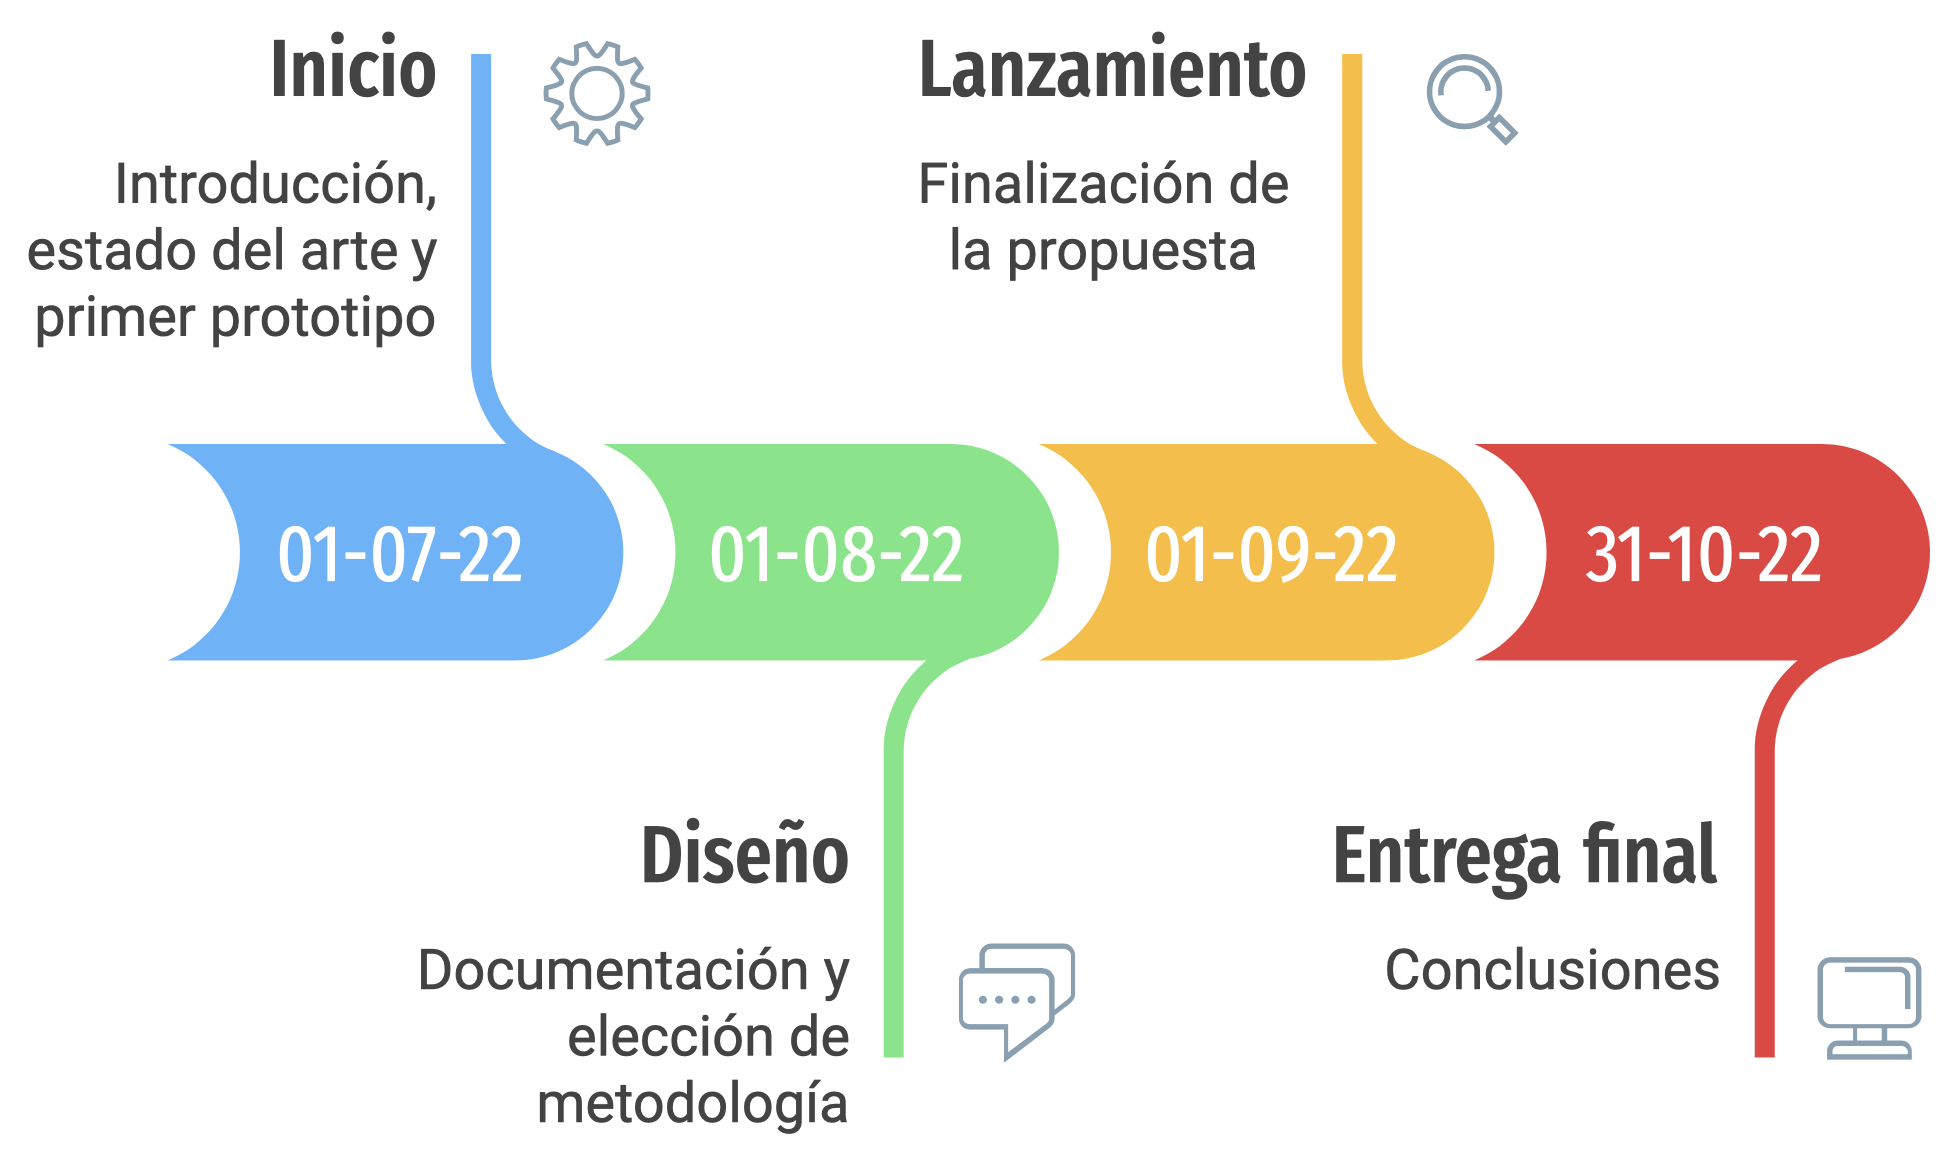
\includegraphics[width=0.9\textwidth]{gfx/plan-simple.png}
    \caption[Planificación inicial del proyecto.]{Visión general sobre la estructura de la elaboración del proyecto.}\label{gfx:plan-simple}

\end{figure}

\newpage

\begin{itemize}
    \item Inicio \textit{(01-07-22 $\sim$ 01-08-22)}: etapa de planificación de la memoria y el estado del arte. Además se intentará tener un primer prototipo de la aplicación.
    \item Diseño \textit{(01-08-22 $\sim$ 01-09-22)}: inicios de la codificación y la elaboración de la parte correspondiente de la memoria.
    \item Lanzamiento \textit{(01-09-22 $\sim$ 01-10-22)}: etapa donde se realizarán pruebas de usuario y finalizará la codificación.
    \item Entrega final \textit{(01-10-22 $\sim$ 31-10-22)}: elaboración de conclusiones respecto al cumplimiento del software y sus posibles mejoras.
\end{itemize}

\section{Planificación detallada}\label{ch:planificacion_detallada}

Al planificar el proyecto de la manera que está representado en la figura \ref{gfx:plan-simple}, he optado por una metodología ágil para confrontar el proyecto.

\vspace{0.3cm}

Esto es debido a que necesitamos un marco de trabajo que sea adaptativo y flexible a la hora de realizar distintas pruebas y su correspondiente arreglo a la hora de encontrarnos errores o cambios exigidos por el cliente.

\vspace{0.3cm}

Todas estas ventajas son las que me encaminado a elegir esta metodología, la cual parece tener las mejores prácticas para este proyecto en concreto.

\vspace{0.3cm}

Hoy en día, el marco de trabajo más ampliamente conocido y a la vez el más ventajoso sea posiblemente SCRUM. Se ha elegido este marco de trabajo para tener el mejor resultado posible a la hora de abarcar el proyecto. Sus principales ventajas son la flexibilidad y la productividad, pero abarcaremos más en detalle sus propiedades en la sección \ref{sec:metodologia}.

\vspace{0.3cm}

En la siguiente página se podrá ver la planificación en mucho mayor detalle. En la tabla (figura \ref{gfx:plan-detallado}) se detalla toda la perspectiva del trabajo, desde las partes más fundamentales de la documentación hasta el diseño de la propia aplicación.

\begin{figure}[hbtp]

    \myfloatalign
    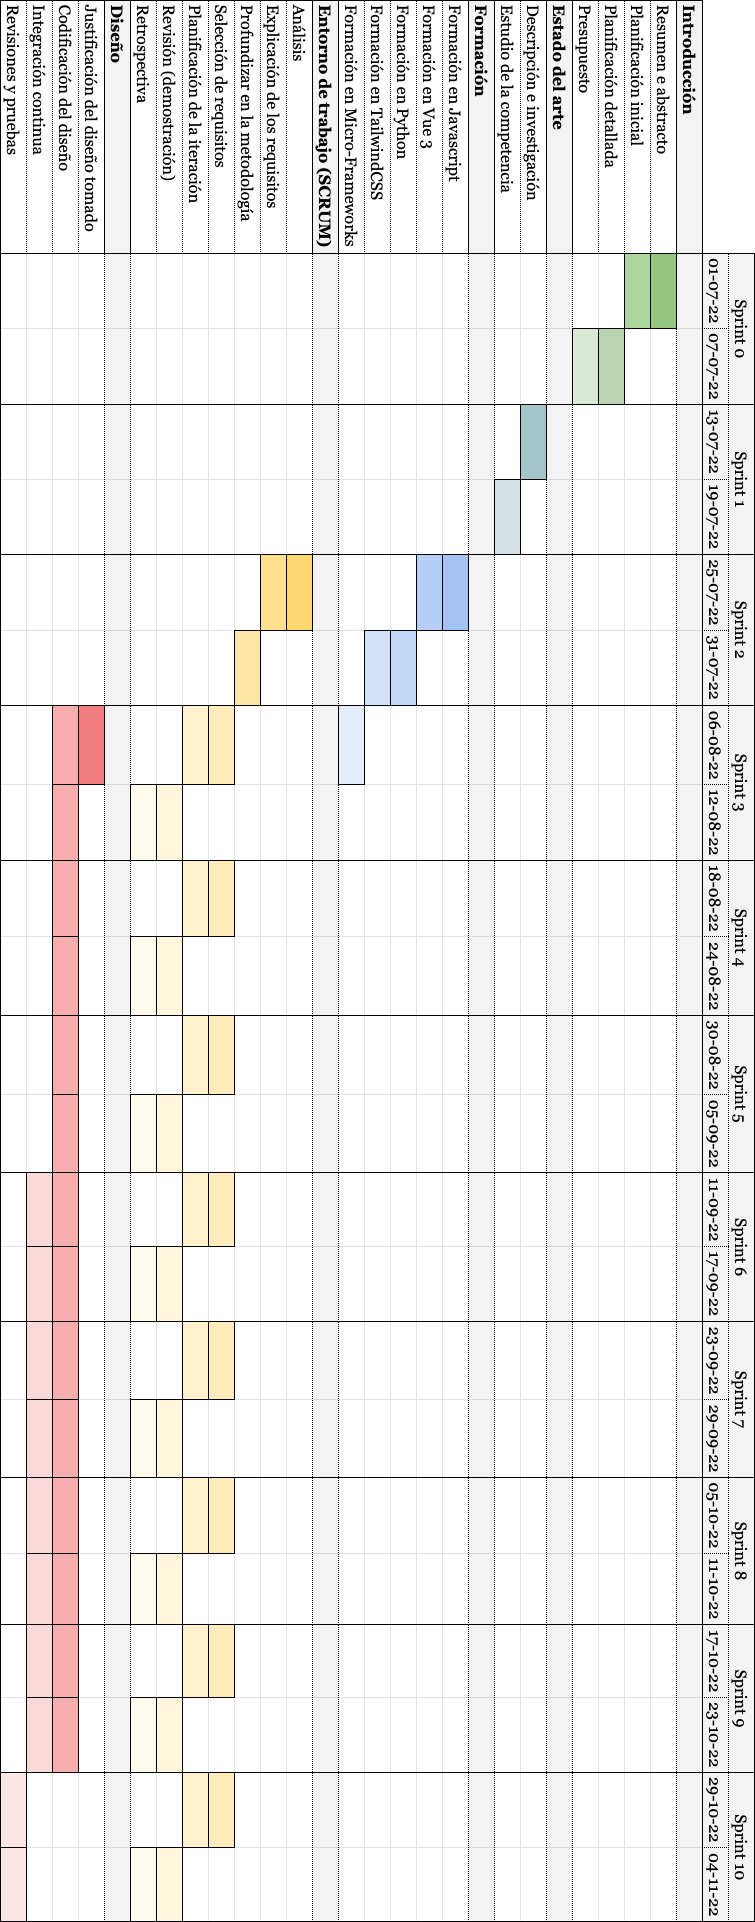
\includegraphics[width=0.73\textwidth]{gfx/plan-detallado.png}
    \caption[Planificación detallada del proyecto.]{Visión más detallada sobre la estructura de la elaboración del proyecto.}\label{gfx:plan-detallado}

\end{figure}

\newpage

\section{Presupuesto}

Las horas de trabajo las tenemos especificadas desde un principio, es decir, el trabajo de fin de grado por normativa tiene 300 horas. Gracias a las páginas web como Talent podemos saber que el salario medio de un desarrollador web está en torno de los 11,79 €. \cite{Salario-Desarrollador-Web} En cuanto a las horas de trabajo y sus diferentes secciones quedaría de la siguiente manera.

\vspace{0.3cm}

\begin{table}[h]

    \centering
    \setlength\arrayrulewidth{0.8pt}

    \begin{tabular}{ >{\centering\arraybackslash}m{1.2in} | >{\centering\arraybackslash}m{0.8in} | >{\centering\arraybackslash}m{0.8in} | >{\centering\arraybackslash}m{0.8in} |}

\cline{2-4}
                                                                          & \cellcolor{RoyalBlue}{Horas} & \cellcolor{RoyalBlue}{Porcentaje} & \cellcolor{RoyalBlue}{Coste} \\ \hline
\multicolumn{1}{|c|}{\cellcolor{RoyalBlue}\textbf{Introducción}}       & $16.9014$                                              & $5.6338$ \%                                                 & $199.27$ €                                             \\ \hline
\multicolumn{1}{|c|}{\cellcolor{RoyalBlue}\textbf{Estado del arte}}    & $8.4507$                                               & $2.8169$ \%                                                 & $99.64$ €                                              \\ \hline
\multicolumn{1}{|c|}{\cellcolor{RoyalBlue}\textbf{Formación}}          & $21.1267$                                              & $7.0422$ \%                                                 & $249.08$ €                                             \\ \hline
\multicolumn{1}{|c|}{\cellcolor{RoyalBlue}\textbf{Entorno de trabajo}} & $147.8873$                                             & $49.2957$ \%                                                & $1743.59$ €                                            \\ \hline
\multicolumn{1}{|c|}{\cellcolor{RoyalBlue}\textbf{Diseño}}             & $105.6338$                                             & $35.2112$ \%                                                & $1245.42$ €                                            \\ \hline
\multicolumn{1}{|c|}{\cellcolor{RoyalBlue}\textbf{Total}}              & $\approx$ $300$                                                & $\approx$ $100$ \%                                                  & $3536.99$ €                                            \\ \hline
\end{tabular}

    \caption[Presupuesto de la mano de obra]{Presupuesto de la mano de obra, junto con las horas trabajadas.}\label{table:presupuesto-obra-de-mano}

\end{table}

En base a ello, podemos calcular que unas 300 horas de trabajo equivaldrían a 3537 € y la elaboración de la documentación o el manual equivaldrían a 300 €. En total 3837 € solamente por la mano de obra.

\vspace{0.3cm}

Buscaré además el uso de herramientas gratuitas de diferentes servicios para el mantenimiento del servicio web. En los servicios como Heroku varían los precios entre 100 € y 200 € al mes, pero también poseen herramientas gratuitas y muy limitadas, lo que nos permitirá un gran ahorro al inicio del proyecto. Igualmente para el proyecto necesitaré un área de trabajo y un ordenador capaz de manejar dicho proyecto.

\vspace{0.3cm}

\begin{table}[h]

    \centering
    \setlength\arrayrulewidth{0.8pt}

    \begin{tabular}{ >{\centering\arraybackslash}m{1.2in} | >{\centering\arraybackslash}m{0.8in} | >{\centering\arraybackslash}m{0.8in} |}

    \cline{2-3}
                                                                              & \cellcolor{RoyalBlue}{Cantidad} & \cellcolor{RoyalBlue}{Coste} \\ \hline
    \multicolumn{1}{|c|}{\cellcolor{RoyalBlue}\textbf{Espacio de trabajo}} & $4$ meses                                                 & $\approx$ $400$ €                                                \\ \hline
    \multicolumn{1}{|c|}{\cellcolor{RoyalBlue}\textbf{Ordenador}}          & $1$                                                       & $\approx$ $900$ €                                                \\ \hline
    \multicolumn{1}{|c|}{\cellcolor{RoyalBlue}\textbf{Total}}              &                                                         & $\approx$ $1300$ €                                               \\ \hline
    \end{tabular}

    \caption[Presupuesto de servicios adicionales]{Presupuesto de servicios adicionales, junto con las diferentes cantidades.}\label{table:presupuesto-adicional}

\end{table}

De modo, que el coste total del proyecto sería la suma de ambas cantidades. En este caso, quedaría en 5137 €.
	\chapter{Planificación}\label{ch:planificacion}
%************************************************

\section{Planificación inicial}
La planificación mostrada a continuación fue realizada al inicio del proyecto, siendo ésta de muy alto nivel. De momento no vamos a indagar en detalles específicos sobre las metodologías usadas o la planificación real, esto en cambio, se detallará en la sección posterior.

\vspace{0.3cm}

Un trabajo de fin de grado está compuesto por 12 créditos en el Título de Grado en Ingeniería Informática de la Universidad de Granada. Además, por normativa de la universidad, a cada crédito ECTS se le establece un número de 25 horas de trabajo. En total, 300 horas de trabajo. Esto se traduce a casi dos meses de trabajo si contamos con una jornada laboral completa y descanso los fines de semana.

\vspace{0.3cm}

Aunque, al fin y al cabo, sigue siendo una estimación muy ligera a lo que realmente terminará siendo. Por lo que la estimación que usaré a continuación será en base a las fechas del inicio y el fin de la elaboración del proyecto, en mi caso será desde inicios de Julio hasta finales de Octubre:

\vspace{0.3cm}

\begin{figure}[bth]

    \myfloatalign
    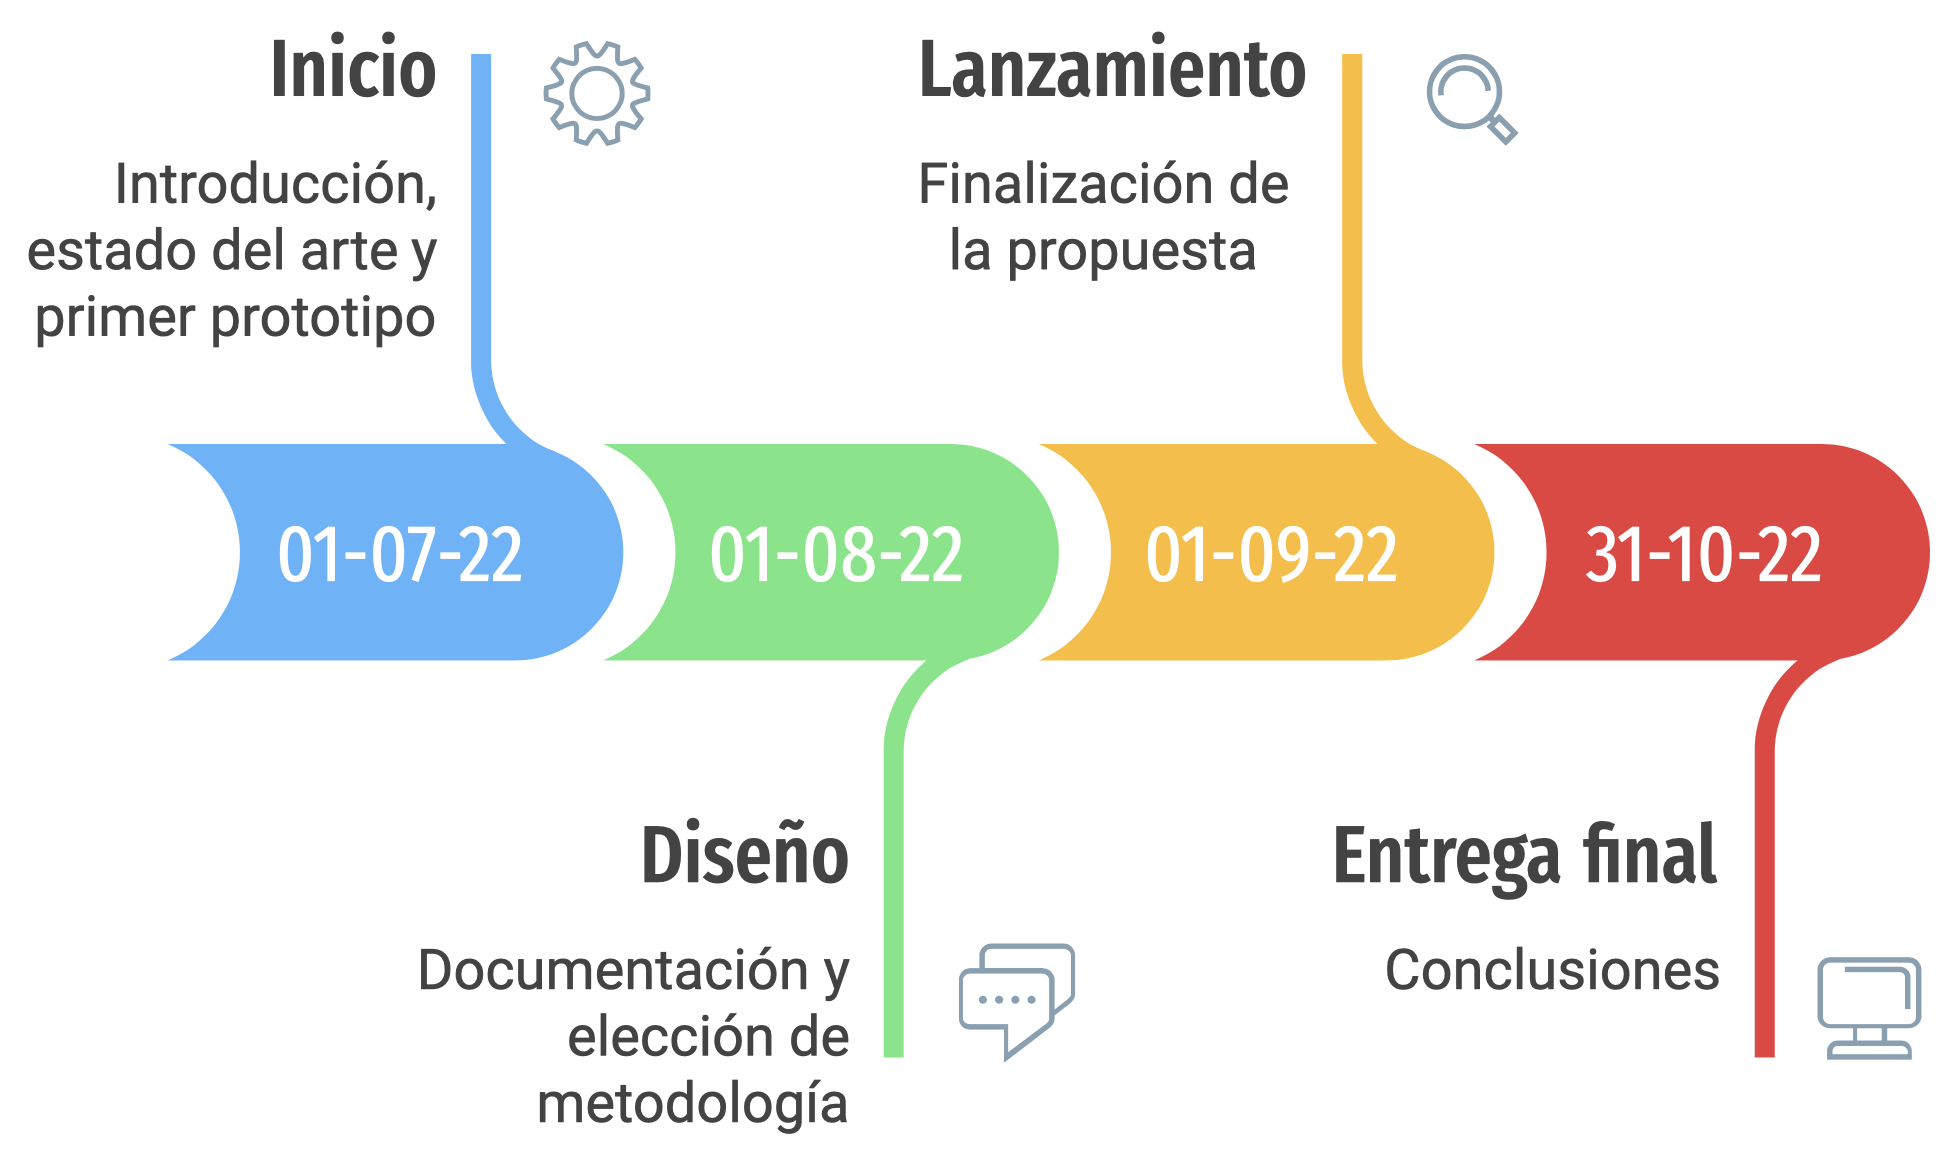
\includegraphics[width=0.9\textwidth]{gfx/plan-simple.png}
    \caption[Planificación inicial del proyecto]{Visión general sobre la estructura de la elaboración del proyecto.}\label{gfx:plan-simple}

\end{figure}

\newpage

\begin{itemize}
    \item Inicio \textit{(01-07-22 $\sim$ 01-08-22)}: etapa de planificación de la memoria y el estado del arte. Además, se intentará tener un primer prototipo de la aplicación.
    \item Diseño \textit{(01-08-22 $\sim$ 01-09-22)}: inicios de la codificación y la elaboración de la parte correspondiente de la memoria.
    \item Lanzamiento \textit{(01-09-22 $\sim$ 01-10-22)}: etapa donde se realizarán pruebas de usuario y finalizará la codificación.
    \item Entrega final \textit{(01-10-22 $\sim$ 31-10-22)}: elaboración de conclusiones respecto al cumplimiento del software y sus posibles mejoras.
\end{itemize}

\section{Planificación detallada}\label{ch:planificacion_detallada}

Al planificar el proyecto de la manera que está representado en la figura \ref{gfx:plan-simple}, he optado por una metodología ágil para confrontar el proyecto.

\vspace{0.3cm}

Esto es debido a que necesitamos un marco de trabajo que sea adaptativo y flexible a la hora de realizar distintas pruebas y su correspondiente arreglo a la hora de encontrarnos errores o cambios exigidos por el cliente.

\vspace{0.3cm}

Todas estas ventajas son las que me encaminado a elegir esta metodología, la cual parece tener las mejores prácticas para este proyecto en concreto.

\vspace{0.3cm}

Hoy en día, el marco de trabajo más ampliamente conocido y a la vez el más ventajoso sea posiblemente SCRUM. Se ha elegido este marco de trabajo para tener el mejor resultado posible a la hora de abarcar el proyecto. Sus principales ventajas son la flexibilidad y la productividad, pero abarcaremos más en detalle sus propiedades en la sección \ref{sec:metodologia}.

\vspace{0.3cm}

En la siguiente página se podrá ver la planificación en mucho mayor detalle. En la tabla (figura \ref{gfx:plan-detallado}) se detalla toda la perspectiva del trabajo, desde las partes más fundamentales de la documentación hasta el diseño de la propia aplicación.

\begin{figure}[hbtp]

    \myfloatalign
    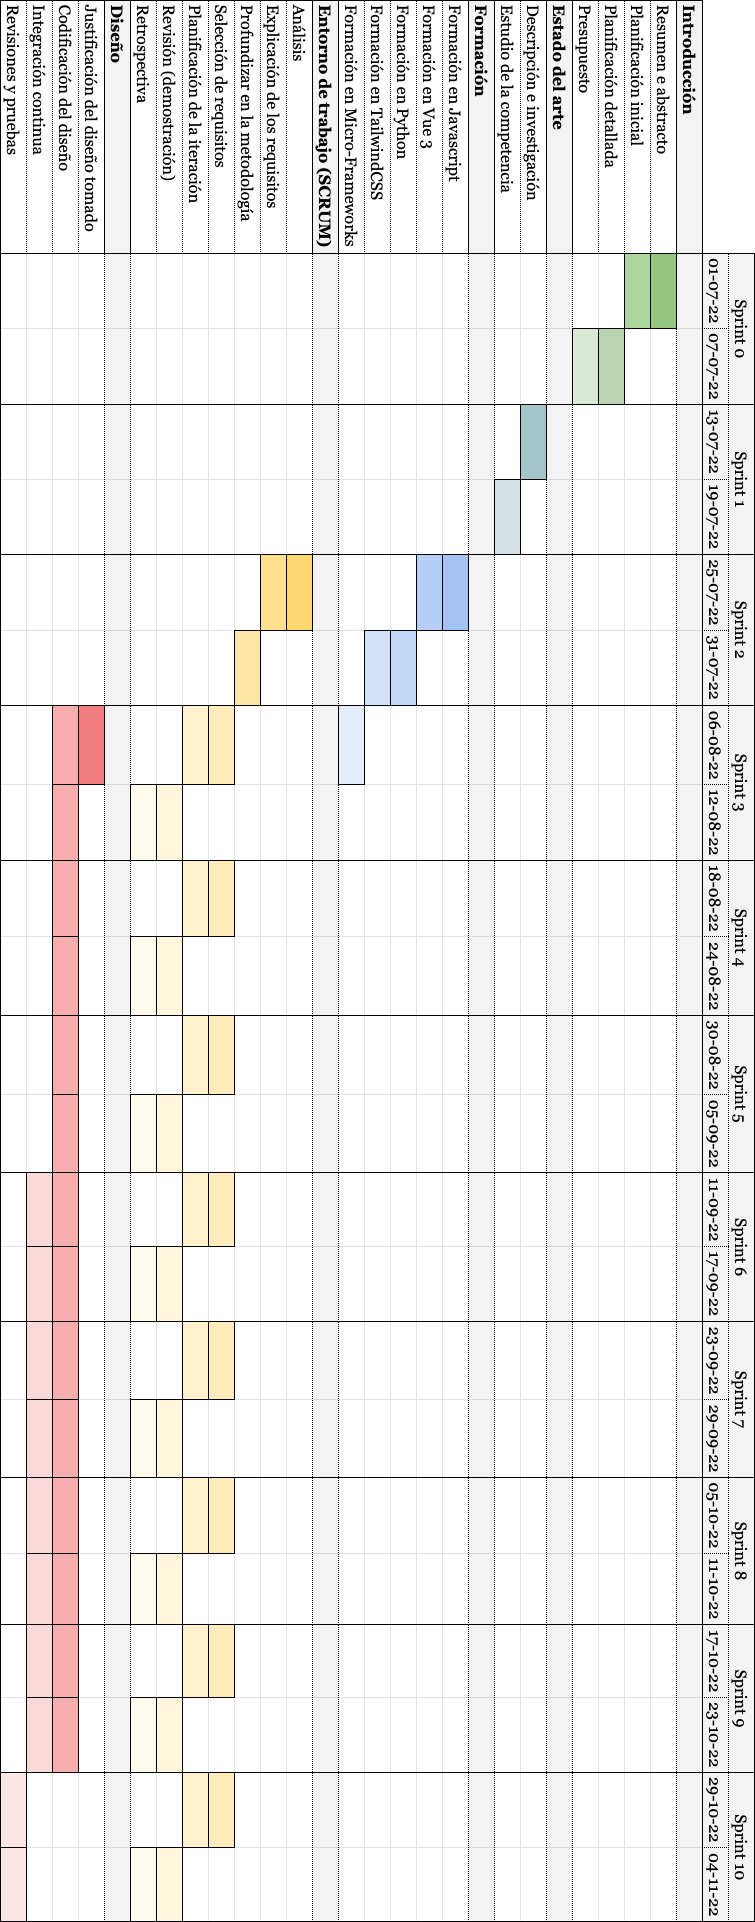
\includegraphics[width=0.73\textwidth]{gfx/plan-detallado.png}
    \caption[Planificación detallada del proyecto]{Visión más detallada sobre la estructura de la elaboración del proyecto.}\label{gfx:plan-detallado}

\end{figure}

\newpage

\section{Presupuesto}

Las horas de trabajo las tenemos especificadas desde un principio, es decir, el trabajo de fin de grado por normativa tiene 300 horas. Gracias a las páginas web como Talent podemos saber que el salario medio de un desarrollador web está en torno de los 11,79 €. \cite{Salario-Desarrollador-Web} En cuanto a las horas de trabajo y sus diferentes secciones quedaría de la siguiente manera.

\vspace{0.3cm}

\begin{table}[h]

    \centering
    \setlength\arrayrulewidth{0.8pt}

    \begin{tabular}{ >{\centering\arraybackslash}m{1.2in} | >{\centering\arraybackslash}m{0.8in} | >{\centering\arraybackslash}m{0.8in} | >{\centering\arraybackslash}m{0.8in} |}

\cline{2-4}
                                                                          & \cellcolor{RoyalBlue}{Horas} & \cellcolor{RoyalBlue}{Porcentaje} & \cellcolor{RoyalBlue}{Coste} \\ \hline
\multicolumn{1}{|c|}{\cellcolor{RoyalBlue}\textbf{Introducción}}       & $16.9014$                                              & $5.6338$ \%                                                 & $199.27$ €                                             \\ \hline
\multicolumn{1}{|c|}{\cellcolor{RoyalBlue}\textbf{Estado del arte}}    & $8.4507$                                               & $2.8169$ \%                                                 & $99.64$ €                                              \\ \hline
\multicolumn{1}{|c|}{\cellcolor{RoyalBlue}\textbf{Formación}}          & $21.1267$                                              & $7.0422$ \%                                                 & $249.08$ €                                             \\ \hline
\multicolumn{1}{|c|}{\cellcolor{RoyalBlue}\textbf{Entorno de trabajo}} & $147.8873$                                             & $49.2957$ \%                                                & $1743.59$ €                                            \\ \hline
\multicolumn{1}{|c|}{\cellcolor{RoyalBlue}\textbf{Diseño}}             & $105.6338$                                             & $35.2112$ \%                                                & $1245.42$ €                                            \\ \hline
\multicolumn{1}{|c|}{\cellcolor{RoyalBlue}\textbf{Total}}              & $\approx$ $300$                                                & $\approx$ $100$ \%                                                  & $3536.99$ €                                            \\ \hline
\end{tabular}

    \caption[Presupuesto de la mano de obra]{Presupuesto de la mano de obra, junto con las horas trabajadas.}\label{table:presupuesto-obra-de-mano}

\end{table}

En base a ello, podemos calcular que unas 300 horas de trabajo equivaldrían a 3537 € y la elaboración de la documentación o el manual equivaldrían a 300 €. En total 3837 € solamente por la mano de obra.

\vspace{0.3cm}

Buscaré además el uso de herramientas gratuitas de diferentes servicios para el mantenimiento del servicio web. En los servicios como Heroku varían los precios entre 100 € y 200 € al mes, pero también poseen herramientas gratuitas y muy limitadas, lo que nos permitirá un gran ahorro al inicio del proyecto. Igualmente, para el proyecto cubriré necesidades básicas, como un área de trabajo y un ordenador capaz de manejar dicho proyecto.

\vspace{0.3cm}

\begin{table}[h]

    \centering
    \setlength\arrayrulewidth{0.8pt}

    \begin{tabular}{ >{\centering\arraybackslash}m{1.2in} | >{\centering\arraybackslash}m{0.8in} | >{\centering\arraybackslash}m{0.8in} |}

    \cline{2-3}
                                                                              & \cellcolor{RoyalBlue}{Cantidad} & \cellcolor{RoyalBlue}{Coste} \\ \hline
    \multicolumn{1}{|c|}{\cellcolor{RoyalBlue}\textbf{Espacio de trabajo}} & $4$ meses                                                 & $\approx$ $400$ €                                                \\ \hline
    \multicolumn{1}{|c|}{\cellcolor{RoyalBlue}\textbf{Ordenador}}          & $1$                                                       & $\approx$ $900$ €                                                \\ \hline
    \multicolumn{1}{|c|}{\cellcolor{RoyalBlue}\textbf{Total}}              &                                                         & $\approx$ $1300$ €                                               \\ \hline
    \end{tabular}

    \caption[Presupuesto de servicios adicionales]{Presupuesto de servicios adicionales, junto con las diferentes cantidades.}\label{table:presupuesto-adicional}

\end{table}

De modo, que el coste total del proyecto sería la suma de ambas cantidades. En este caso, quedaría en 5137 €.
	\part{Propuesta}\label{pt:propuesta}
	\chapter{Análisis}\label{ch:analisis}
%************************************************

\section{Metodología de desarrollo}\label{sec:metodologia}

El proceso de desarrollo de un software puede llegar a ser una tarea muy ardua, durante mucho tiempo esta labor se ha llevado a cabo sin ninguna metodología definida. Para situar el contexto, una metodología se define como una colección de procedimientos, técnicas, herramientas y documentos que llegan a ayudar a los desarrolladores a la hora de implementar software. \cite{gomez2010criterios}

\vspace{0.3cm}

Durante las últimas décadas, se han establecido dos grandes corrientes diferenciales que representan estas metodologías. Por un lado, las metodologías tradicionales se centran en el proceso y controlan estrictamente las actividades que lo acompañan. Las metodologías ágiles, por otro lado, se enfocan en el elemento humano, centrándose en la colaboración y participación del cliente en el proceso a través de iteraciones muy cortas. \cite{gomez2010criterios}

\begin{table}[h]
    \footnotesize
    \centering
    \setlength\arrayrulewidth{0.8pt}
    \begin{tabular}{| >{\centering\arraybackslash}m{2in} | >{\centering\arraybackslash}m{2in} |}

        \hline
        \rowcolor{RoyalBlue}
        \textbf{Metodologías Ágiles} & \textbf{Metodologías Tradicionales} \\
        \hline
        Basadas en heurísticas provenientes de prácticas de producción de código & Basadas en normas provenientes de estándares seguidos por el entorno de desarrollo \\
        \hline
        Especialmente preparados para cambios durante el proyecto & Cierta resistencia a los cambios \\
        \hline
        Impuestas internamente (por el equipo) & Impuestas externamente \\
        \hline
        Proceso menos controlado, con pocos principios & Proceso mucho más controlado, con numerosas políticas/normas \\
        \hline
        No existe contrato tradicional o al menos es bastante flexible & Existe un contrato prefijado \\
        \hline
        El cliente es parte del equipo de desarrollo & El cliente interactúa con el equipo de desarrollo mediante reuniones \\
        \hline
        Grupos pequeños (menos de 10 integrantes) y trabajando en el mismo sitio & Grupos grandes y posiblemente distribuidos \\
        \hline
        Pocos artefactos y pocos roles & Más artefactos y más roles \\
        \hline
        Menos énfasis en la arquitectura del software & La arquitectura del software es esencial y se expresa mediante modelos \\
        \hline
        
    \end{tabular}

    \caption[Comparación de metodologías]{Comparación de metodologías. \cite{canos2003metodologias}}\label{table:comparacion_metodologias}

\end{table}

La parte más importante de las fases iniciales es poder determinar qué metodología es mejor para nuestro proyecto con el fin de lograr los mejores resultados de manera oportuna.

\vspace{0.3cm}

El objetivo general de implementar una metodología es llegar a construir un producto de alta calidad. Esta elección implica un conjunto de principios básicos que deben ser seguidos y respetados. Estos incluyen actividades claras para comprender el problema y comunicarse con los clientes, un método definido para representar el diseño, las mejores prácticas para implementar la solución y estrategias sólidas. \cite{maida2015metodologias}

\vspace{0.3cm}

En base a las características mencionadas y lo explicado en la sección de planificación, se ha considerado que la solución óptima sería una metodología de desarrollo ágil. Considerando que el problema puede cambiar a lo largo del proyecto, por lo que necesitamos una metodología adaptativa y flexible, además la forma de trabajar concuerda mucho más (la cantidad del grupo o su propio manejo).

\subsection{Metodología de trabajo escogida (SCRUM)}
El nacimiento de la idea de la metodología Scrum fue en el año 1986, con el propósito de aumentar la velocidad de desarrollo de una aplicación y a la vez conservando flexibilidad. Los japonenses Hirotaka Takeuchi e Ikujiro Nonaka  se inspiraron en el concepto de un equipo de rugby de 15 jugadores unido y con el mismo objetivo. Durante los años posteriores este concepto fue remodelado y reforzado hasta convertirse en lo que es a día de hoy, el método ágil más usado en el mundo. \cite{rodriguez2015que}

\vspace{0.3cm}

Scrum puede llegar a ser ventajoso debido a que el cliente se siente comprometido con el proyecto, implicándose en distintas necesidades de tipo funcional y permitiendo realizar revisiones tempranas de los desarrollos fomentando de esta manera las propias entregas. Otras ventajas a destacar pueden llegar a ser su adaptación o trabajo en equipo. \cite{rodriguez2015que}

\vspace{0.3cm}

Los componentes de la metodología Scrum son: \cite{rad2019fundamentos}

\begin{enumerate}

    \item
    Los \textbf{Roles de Scrum}: son los papeles o funciones de cada integrante del equipo, que puede ser:
    
        \begin{itemize}
            \item
            \textit{El Dueño del Producto (Product Owner)}: representará la función del cliente, con el objetivo de definir historias de usuario y validar la calidad del producto.
    
            \item
            \textit{Scrum Master}: su función es velar por la actividad o ejecución del Scrum, para que se realice correctamente por el equipo. También será el responsable de dirigir y concretar los diferentes eventos.
    
            \item
            \textit{El Equipo de Desarrollo}: son los que tienen la función de realizar y concretar las historias de usuario.
    
            \item
            \textit{Stakeholders}: no tienen función en la ejecución o realización del trabajo, pero están interesados en el producto y represan un papel de suma importancia.
    
        \end{itemize}

    \item
    Los \textbf{Eventos Scrum}: son las reuniones que se llevan a cabo en el equipo de trabajo. Están diseñados para la comunicación y colaboración continua entre equipos, con el objetivo de minimizar la necesidad de mantener reuniones indefinidas que pueden afectar de alguna manera a la planificación del proyecto. Se subdividen en estos tipos:

        \begin{itemize}
            \item
            \textit{El Sprint}: trata de un tramo de tiempo fijo, que puede llegar a ser entre una y cuatro semanas, durante el cual el producto que se esté desarrollando añade valor gradualmente, de manera que al final de cada sprint el cliente pueda tener una clara visión del producto.
    
            \item
            \textit{La planificación del Sprint (Sprint Planning)}: es una reunión que se lleva a cabo al comienzo o inicio de cada sprint para planificar el trabajo que se realizará a lo largo del sprint.
    
            \item
            \textit{Scrum Diario (Dailys)}: reuniones diarias de corta duración, en estas reuniones los miembros del equipo discuten y dialogan el trabajo realizado en el día anterior y el trabajo que se realizará en el día de la reunión.
    
            \item
            \textit{Revisión del Sprint (Sprint Review)}: una reunión donde cada miembro del equipo presenta lo que ha realizado a lo largo del sprint y lo que debería cambiar o mejorar en el producto para el próximo sprint.

            \item
            \textit{Retrospectiva del Sprint (Sprint Retrospective)}: reuniones con la intención de analizar el trabajo en equipo y discutir áreas para mejorar o colaborar como equipo para el próximo sprint.
    
        \end{itemize}

    \item
    Los \textbf{Artefactos de Scrum}: utilizadas para aumentar la transparencia de la información para que todos los miembros del equipo tengan constancia sobre lo que está ocurriendo. Se subdividen en:
    
        \begin{itemize}
            \item
            \textit{El Backlog del Producto (Product Backlog)}: contienen todas las historias de usuario, pero no evalúan el proyecto, y su gestión o responsabilidad recae en el Dueño del Producto.
    
            \item
            \textit{El Backlog del Sprint (Sprint Backlog)}: historias de usuario que contienen estimaciones y planes a realizar en el sprint.
    
            \item
            \textit{Incremento}: es el producto que se produce o ocurre al final del sprint.
    
        \end{itemize}

\end{enumerate}

\vspace{0.3cm}

\subsection{Adaptación de la metodología de trabajo escogida}
Habiendo definido los componentes en la sección anterior, es visible que Scrum está dirigido para trabajar en equipo, por lo que se tendrá que adaptar esta metodología al entorno académico del proyecto, que en el caso de este proyecto se reduciría a mi persona, Nikita Stetskiy. Debido a esto, me veré obligado a representar todos los roles del equipo y mis tutores darán función a los stakeholders y a Scrum Master.

\vspace{0.3cm}

Además, se puede dividir el proyecto en dos productos. La memoria, donde el cliente será el tribunal del trabajo de fin de grado y los tutores serán los Dueños del Producto. Mientras que para la propia aplicación, tendremos un cliente ficticio, por ejemplo Mauricio Mares, y el Dueño del Producto seré yo mismo, puesto que seré el que mejor conoceré los intereses del cliente.

\vspace{0.3cm}

En cuanto a los eventos, el Scrum diario no llega a tener sentido en este entorno, al estar formado por solo una persona y los demás eventos se pueden juntar en un mismo encuentro e iteración.

\vspace{0.3cm}

Finalmente, respecto a la velocidad del proyecto, se llegó a detallar en la sección \ref{ch:planificacion_detallada} de la Planificación. Cada Sprint tiene acordada una duración de dos semanas.

\newpage
\section{Análisis del entorno}

Es necesario estudiar el entorno y a los posibles usuarios que necesiten de nuestro servicio antes de empezar a desarrollar el \textit{Backlog} del Producto. Para ello propondré dos diferentes casos ficticios que estudiaremos a continuación.

\begin{table}[h]
\centering
    \begin{tabular}{| >{\centering\arraybackslash}m{0.75in} >{\centering\arraybackslash}m{3.5in}|}
        \hline
\multicolumn{2}{|c|}{\cellcolor{RoyalBlue}\textbf{1ª Persona}}                                                                                                                                                                                                                                                                                                                                                                                                                      \\ \hline
\multicolumn{1}{|c|}{\textbf{Nombre}}                                                                                                                                                                                                                  & Mauricio Mares                                                                                                                                                                                                                \\ \hline
\multicolumn{1}{|c|}{\textbf{Edad}}                                                                                                                                                                                                                    & 23                                                                                                                                                                                                                            \\ \hline
\multicolumn{1}{|c|}{\textbf{Sexo}}                                                                                                                                                                                                                    & Masculino                                                                                                                                                                                                                     \\ \hline
\multicolumn{2}{|c|}{\textbf{Datos relevantes}}                                                                                                                                                                                                                                                                                                                                                                                                                                        \\ \hline
\multicolumn{2}{|p{4.25in}|}{Terminó la carrera de bellas artes, aunque ahora mismo no se siente lo suficientemente apasionado para trabajar de ello. Uno de los principales motivos es el sobreúso de las redes sociales en su día a día.}                                                                                                                                                                                                                                                    \\ \hline
\multicolumn{2}{|c|}{\textbf{Contexto de uso}}                                                                                                                                                                                                                                                                                                                                                                                                                                         \\ \hline
\multicolumn{2}{|p{4.25in}|}{El uso que pretende dar este usuario corresponde a un ámbito casual, ya que pretende usar menos las redes sociales, pero a la par quiere mantenerse actualizado de lo que pasa en el mundo. Por lo que la función que requiere de la aplicación es de informarse de eventos importantes que transcurran diariamente o incluso semanalmente.}                                                                                                                                                         \\ \hline
\multicolumn{2}{|c|}{\textbf{Necesidad diferencial}}                                                                                                                                                                                                                                                                                                                                                                                                                                   \\ \hline
\multicolumn{2}{|p{4.25in}|}{La funcionalidad a destacar es que la aplicación deberá guardar todas las tendencias del día y poder dar datos que resuman información de dichas tendencias. Además, Mauricio no tiene que estar constantemente atento a la aparición de una nueva tendencia, ya que se van guardando por días. Esto le permitirá a Mauricio reducir las horas de consumo diario de aplicaciones que requerían su atención constante a cambio de información relevante o actual.} \\ \hline
\end{tabular}
\caption[Primer caso de estudio de entorno]{Primer caso de estudio de entorno.}\label{table:1-entorno-persona}
\end{table}

En este primer caso necesitamos que la aplicación sea capaz de resumir información de tendencias diarias y que a la vez no sea atosigante o que agobie con demasiada cantidad de información, por ende, tiene que ser información simple y finita. La posible solución más óptima es organizar tendencias diarias en un \textit{top} o una clasificación de diez tendencias más populares ocurridas a lo largo del día. Además, esto se puede guardar por semanas para que el usuario no tenga la obligación de entrar a la web diariamente.

\vspace{0.3cm}

El carácter de la información, simplificada para el usuario que tendrán las tendencias, será puramente informativo y además intentará ser objetiva. La principal diferencia es que al usar las \ac{RRSS}, la información relevante se consigue por medio de la atención. Cuantas más publicaciones u opiniones de personas se lean, más informado estará el usuario. Por lo que el factor diferencial, es que la página web en desarrollo mostrará datos simplificados o resumidos de manera objetiva. Todos estos datos estarán comprimidos de tal manera, que el usuario pueda tener una visión clara sobre la tendencia sin la necesidad de leer un alto número de publicaciones u opiniones.

\vspace{0.3cm}

La información que se aporta al usuario en la aplicación web será modular. De tal manera que cada módulo, que tendrá el diseño de una carta, informará de un dato de interés. Los datos más importantes que puede tener una tendencia y que sea útil para el usuario son datos como la relevancia que está teniendo la tendencia, las palabras o \textit{keywords} más usadas, las opiniones de las personas (vistas de manera objetiva a través de un análisis de sentimientos) y diferentes noticias actuales relacionadas con la propia tendencia.

\vspace{0.3cm}

De esta manera, al aportar información de manera simplificada, el usuario Mauricio podrá informarse diariamente de manera adecuada y sin la necesidad de perder el tiempo en las \ac{RRSS}.


\begin{table}[h]
\centering
    \begin{tabular}{| >{\centering\arraybackslash}m{0.75in} >{\centering\arraybackslash}m{3.5in}|}
        \hline
\multicolumn{2}{|c|}{\cellcolor{RoyalBlue}\textbf{2ª Persona}}                                                                                                                                                                                                                                                                                                                                                                                                                      \\ \hline
\multicolumn{1}{|c|}{\textbf{Nombre}}                                                                                                                                                                                                                  & Nuria Nevadas                                                                                                                                                                                                                \\ \hline
\multicolumn{1}{|c|}{\textbf{Edad}}                                                                                                                                                                                                                    & 37                                                                                                                                                                                                                            \\ \hline
\multicolumn{1}{|c|}{\textbf{Sexo}}                                                                                                                                                                                                                    & Femenino                                                                                                                                                                                                                     \\ \hline
\multicolumn{2}{|c|}{\textbf{Datos relevantes}}                                                                                                                                                                                                                                                                                                                                                                                                                                        \\ \hline
\multicolumn{2}{|p{4.25in}|}{Terminó hace mucho el grado de Empresariales, en los últimos meses empezó a invertir en Bolsa, por su propia cuenta de manera profesional.}                                                                                                                                                                                                                                                    \\ \hline
\multicolumn{2}{|c|}{\textbf{Contexto de uso}}                                                                                                                                                                                                                                                                                                                                                                                                                                         \\ \hline
\multicolumn{2}{|p{4.25in}|}{El uso que pretende dar este usuario corresponde a un ámbito profesional. Pretende tener una visión pequeña y objetiva de búsquedas concretas, en este caso del mercado financiero.}                                                                                                                                                         \\ \hline
\multicolumn{2}{|c|}{\textbf{Necesidad diferencial}}                                                                                                                                                                                                                                                                                                                                                                                                                                   \\ \hline
\multicolumn{2}{|p{4.25in}|}{La funcionalidad a destacar en esta aplicación es que se podrá buscar tópicos y obtener la misma información actual que se obtienen también con las tendencias, es decir, datos de interés objetivos.} \\ \hline
\end{tabular}
\caption[Segundo caso de estudio de entorno]{Segundo caso de estudio de entorno.}\label{table:1-entorno-persona}
\end{table}

Al estudiar el segundo caso, la solución que se le plantea al usuario llega a ser bastante parecida al primer caso. El principal factor diferencial es que la información que se aporta en el primer caso es sobre las tendencias y en este caso tendrá que ser sobre búsquedas específicas.

\vspace{0.3cm}

No se podrá dar información sobre la popularidad del tópico, ya que no es una tendencia, pero si información sobre las \textit{keywords} o palabras más usadas, el sentimiento general y las noticias más destacables. Esta información tendrá que ser recopilada de distintas publicaciones que tengan relevancia con el tópico.

\subsection{Estudio competitivo}

En la actualidad las principales aplicaciones que existen que recopilan tendencias a diario son Google Trends y parcialmente la plataforma de Twitter. Ambas poseen fallos, el principal problema de Twitter se incluye en los riesgos de un uso continuo de una \ac{RRSS} que se explicó anteriormente en la sección \ref{ch:estado-del-arte}. Por otro lado, Google Trends posee multiples problemas a la hora de afrontar nuestras necesidades. Primero, no funciona en todos los países, incluyendo España. Además, no contienen información relevante que pueda resumir una tendencia o el porqué de su relevancia. Aunque Google Trends posea un exhaustivo historial de las búsquedas que ha tenido dicha tendencia, posibles noticias de interés y tópicos similares, no posee el sentimiento general que está teniendo dicha tendencia y tampoco diferentes \textit{keywords} en relación (esto debido a que carece de publicaciones como Twitter). En resumen, ambas aplicaciones principales, tienden a ser incompletas a nuestras necesidades.

\vspace{0.3cm}

También existen otras páginas que usan información de Twitter o Google. Al buscar páginas o aplicaciones web sobre la información de tendencias actuales de Twitter salen resultados como Trendinalia, GetDayTrends o Trends24. Este tipo de páginas web llega a mostrar un contenido puramente estadístico sobre las tendencias, con el uso exclusivo de diagramas o distribuciones globales para explicar el comportamiento de una tendencia.

\vspace{0.3cm}

Realmente este tipo de páginas no indagan en la explicación del contenido de una tendencia para que el usuario pueda estar informado. El objetivo de estas páginas es informar al usuario de datos numéricos que se calculan mientras la tendencia exista, como puede ser la posición de la tendencia respecto a otras durante las últimas 24 horas.

\vspace{0.3cm}

Esto puede llegar a ser información útil si solo quieres saber datos sobre el comportamiento de la tendencia a lo largo de 24 horas. En el caso de nuestra aplicación, aparte de dar datos sobre el comportamiento de la tendencia, tendrá el objetivo de explicar el propósito de la tendencia.

\subsection{Estudio competitivo técnico}\label{sub:estudio-competitivo-tecnico}

Actualmente las librerías más populares sobre recopilación de tendencias actuales son Tweepy y Pytrends, ambas programadas en el lenguaje Python. Dichas librerías distan de ser perfectas, pero cada una tiene características de carácter diferencial.

\vspace{0.3cm}

\begin{itemize}
    \item
    \textbf{Pytrends} \cite{pytrends-manual}
    
    Esta librería es una API no oficial que usa información de Google Trends. Por lo que es una librería que aporta información muy valiosa respecto a diferentes tendencias. Esta librería posee numerosas ventajas, a la par que desventajas. Las siguientes características son los métodos que tiene la librería disponible:
    \begin{enumerate}
    \item \textit{Interés a lo largo del tiempo}: devuelve datos históricos e indexados de las búsquedas sobre una palabra clave. Esta información se muestra en la sección Interés a lo largo del tiempo de Google Trends.
    \item \textit{Interés histórico por hora}: devuelve datos históricos, indexados y por hora de las búsquedas sobre una palabra clave. Envía múltiples solicitudes a Google, cada una de las cuales recupera una semana de datos por hora.
    \item \textit{Interés por región}: devuelve datos sobre el lugar en el que se busca la palabra clave. Información mostrada en la sección Interés por región de Google Trends.
    \item \textit{Temas relacionados}: devuelve datos de las palabras clave relacionadas con una palabra clave proporcionada. Se muestra en la sección Temas relacionados de Google Trends.
    \item \textit{Consultas relacionadas}: devuelve datos de las palabras clave relacionadas con una palabra clave proporcionada. Se muestra en la sección Consultas relacionadas de Google Trends.
    \item \textit{Búsquedas de tendencias}: devuelve datos de las búsquedas de tendencias más recientes. Se muestran en la sección Búsquedas de tendencias de Google Trends.
    \item \textit{Gráficos principales}: devuelve los datos de un tema determinado. Se muestra en la sección Gráficos principales de Google Trends.
    \item \textit{Sugerencia}: devuelve una lista de palabras clave sugeridas adicionales que se pueden usar para refinar una búsqueda de tendencia.
    \end{enumerate}

    Estas características pueden llegar a ser extremadamente útiles a la hora de gestionar nuestra aplicación. Aunque las principales desventajas son demasiado grandes como para no tenerlas en cuenta:

    \begin{enumerate}
    \item \textit{Disponibilidad geográfica}: debido a ciertas leyes y normativas, Google Trends no funciona en todos los países del mundo. Por desgracia, España está excluida de momento, aunque se tiene pensado cambiar la normativa o adaptarse a ella.
    \item \textit{Longevidad}: esta API al no ser oficial, no tiene garantía de estar funcionando siempre. Ya que llegará un momento donde se cambie el \textit{Back-End} de Google e incidirá en el comportamiento de esta API.
    \item \textit{Limitaciones de llamadas}: El límite de peticiones no se conoce públicamente. Aunque los usuarios hicieron medidas aproximadas, donde se demostraba que 1400 solicitudes secuenciales en un período de tiempo de 4 horas daban lugar al límite (replicado en 2 redes), aunque se podía volver a hacer peticiones después de 60 segundos de tiempo de espera.
    \end{enumerate}

\end{itemize}

\begin{itemize}
    \item
    \textbf{Tweepy} \cite{tweepy-manual}
    
    Es un paquete de código abierto que brinda una forma muy conveniente de acceder a la API de Twitter con Python. Tweepy incluye un conjunto de clases y métodos que representan los modelos de Twitter y los extremos de la API. Las principales características para nuestro uso son las siguientes:
    \begin{enumerate}
    \item \textit{Obtención de tendencias cerca de una ubicación}: devuelve las 50 tendencias principales para un WOEID (código de país) específico, si la información de tendencias está disponible. La respuesta es una lista de objetos "trend" que codifican el nombre del tema de tendencia, el parámetro de consulta que se puede usar para buscar el tema en la búsqueda de Twitter y la URL de búsqueda de Twitter. Esta información se almacena en caché durante 5 minutos.
    \item \textit{Búsqueda de publicaciones}: devuelve una colección de publicaciones o \textit{tweets} relevantes que coinciden con una consulta específica. Aunque la API de búsqueda no pretende ser una fuente exhaustiva de Tweets. No todos los Tweets se indexarán o estarán disponibles a través de la interfaz de búsqueda.
    \end{enumerate}

    Estas características pueden llegar a cumplir las necesidades explicadas anteriormente, aunque también tenemos que tener en cuenta las desventajas que presenta esta API.

    \begin{enumerate}
    \item \textit{Disponibilidad de versiones}: existen actualmente varias versiones de la API publicadas, cada una se accede de una manera diferente y tiene métodos diferentes. La documentación oficial de Twitter no está bien cuidada y no funciona de la misma manera que la aplicación web. Un sencillo ejemplo de ello es que en la web se puede buscar tweets de un país en concreto, mientras que esta función no existe en la API.
    \item \textit{Historial pobre}: mientras que Google guarda todos los datos de interés sobre una tendencia, Twitter no, por lo que búsquedas antiguas no contendrán mucho valor al usuario en cuanto a la relevancia o interés que presenta un tópico.
    \end{enumerate}

\end{itemize}

\subsection{Conclusiones de los estudios realizados}

En los apartados anteriores se definieron claramente las ventajas y desventajas del uso de ambas aplicaciones o APIs. Se puede concluir que, aunque Google Trends posea más funciones versátiles y con mayor peso de utilidad en cuanto a nuestras necesidades, sigue teniendo mayores desventajas a la hora de usarlo. La mayor de todas es que no esté disponible en todos los países. La plataforma de twitter en cambio se usa en casi todo el mundo, además se pueden llegar a implementar funciones parecidas con métodos propios y no tener que depender en un mayor nivel de una API externa.

\vspace{0.3cm}

En cuanto a los aspectos que se deberán tratar a la hora de definir las características o funcionalidades de la aplicación se definirán en la siguiente lista. Aunque se entrará más en detalle en la sección posterior.

\begin{itemize}
    \item
    Las personas requieren información relevante, concisa y simplificada.
    \item
    La información debe ser de contenido finito, a la misma hora aportando al usuario su pleno entendimiento.
    \item
    Los usuarios deberán ser capaces de usar la aplicación en todos los dispositivos que tengan acceso web. Además, deberá tener un diseño \textit{responsive}, para que se adapte a la interfaz del usuario.
    \item
    Los usuarios tienen que ser capaces de navegar a través de distintas tendencias. Poder elegir tanto el país de búsqueda como la fecha para poder informarse debidamente.
    \item
    Los usuarios tienen que ser capaces de realizar búsquedas de distintos tópicos de interés y poder informarse con datos relacionados y actuales.
    \item
    El diseño será presentado mediante módulos o cartas. Cada carta tendrá información útil y de necesidad al usuario.
    \item
    Un módulo contendrá datos sobre la popularidad de la tendencia y su correspondiente gráfico.
    \item
    Otro módulo contendrá datos sobre palabras y \textit{keywords} más usadas sobre la tendencia y su correspondiente gráfico.
    \item
    Otro módulo contendrá un sentimiento general y un gráfico visual sobre dicho comportamiento.
    \item
    También habrá tres módulos de noticias de interés general sobre la tendencia.
    \item
    Cada módulo deberá respetar tanto el idioma como la localización elegida por el usuario.
    \item
    Se deberá tener en cuenta que el diseño sea simple y agradable al usuario.
    \item
    Otro factor a tener en cuenta es el plan de peticiones que ofrece Twitter, el cual es muy limitado.
\end{itemize}

\newpage

\section{Requisitos del sistema}
Gracias a los estudios y conclusiones realizadas en el capítulo anterior, se puede detallar de una manera más sencilla los siguientes requerimientos o requisitos. Los requerimientos funcionales funcionan como servicios que puede prestar el sistema. Mientras que los requerimientos no funcionales especifican más bien la fiabilidad o el comportamiento de este.

\subsection{Requisitos Funcionales}

\begin{enumerate}
    { \renewcommand\labelenumi{R.F. \theenumi}
    \item
    \textit{Gestión de Trends}. El sistema deberá ser capaz de realizar llamadas al servicio de la API de Twitter para recopilar tendencias. En la API o su plataforma se denominan Trends o \ac{TT}.
        \begin{enumerate}{\renewcommand{\labelenumii}{R.F. \arabic{enumi}.\arabic{enumii}}
        \item
        \textit{Gestión de Países}. El sistema deberá ser capaz de manejar la petición concorde a diferentes países y almacenarlas adecuadamente.
            \begin{enumerate}{\renewcommand{\labelenumiii}{R.F. \arabic{enumi}.\arabic{enumii}.\arabic{enumiii}}
            \item
            \textit{Búsqueda por WOEID}. El sistema deberá ser capaz de buscar los diferentes países por el identificador que provee Yahoo y que utiliza la plataforma de Twitter. En este caso se denominan WOEIDs.
            }\end{enumerate}
        \item
        \textit{Gestión de la Fecha}. El sistema deberá ser capaz de manejar la respuesta generada por Twitter y poder diferenciarla por fecha, bajo el formato de yy-mm-dd.
        \item
        \textit{Limpieza de Trends}. El sistema deberá poder limpiar los Trends repetidos. Ya que la mayoría de las veces Twitter no reconoce el mismo \ac{TT}, casos como el uso de tilde, mayúsculas o si son una sucesión de varias palabras. Por ejemplo, «Balón», «balón», «balon» y «Balón de Oro» se referirán a la misma tendencia, pero Twitter los trata como Trends diferentes con datos respectivos diferentes.
        \begin{enumerate}{\renewcommand{\labelenumiii}{R.F. \arabic{enumi}.\arabic{enumii}.\arabic{enumiii}}
            \item
            \textit{Preferencias de Limpieza}. El sistema preferirá un nombre de tendencias más largo y por defecto si son iguales, preferirá el que tenga más popularidad.
            }\end{enumerate}
        \item
        \textit{Ordenación de los Trends}. El sistema deberá ser capaz de ordenar los \ac{TT} bajo el atributo del volumen de popularidad proporcionado por Twitter.
        \item
        \textit{Historial Inteligente}. Además de guardar los Trends ordenados, al usuario le será importante que se guarden y se vayan comparando los Trends viejos y los nuevos (mediante el atributo de la popularidad).
        }\end{enumerate}
    \item
    \textit{Gestión de Popularidad}. El sistema deberá ser capaz de guardar el atributo del volumen de popularidad en una lista, que fue anteriormente proporcionado por Twitter.
    \begin{enumerate}{\renewcommand{\labelenumii}{R.F. \arabic{enumi}.\arabic{enumii}}
        \item
        \textit{Cálculo de Media}. El sistema deberá poder sacar la media o la popularidad promedio a partir de la lista guardada anteriormente.
        \item
        \textit{Cálculo de Moda}. El sistema deberá poder sacar la moda o la popularidad más grande a partir de la lista guardada anteriormente.
        \item
        \textit{Gestión de Hora}. El sistema tiene que guardar en una lista la hora a la que se ha calculado el valor de la popularidad.
        \item
        \textit{Gestión de Gráfico}. Se deberá proporcionar un gráfico a partir de los valores calculados anteriormente. Proporcionado en formato de área.
        \begin{enumerate}{\renewcommand{\labelenumiii}{R.F. \arabic{enumi}.\arabic{enumii}.\arabic{enumiii}}
            \item
            \textit{Eje X}. Se deberá proporcionar la lista de la hora a la que se ha calculado la popularidad como eje X del gráfico.
            \item
            \textit{Eje Y}. Se deberá proporcionar la lista del vector de popularidad como el eje Y del gráfico.
            \item
            \textit{Análisis del Gráfico}. Además del gráfico visual, se deberán proporcionar datos de valor. En este caso, el primer dato calculado y el último, además de mostrar la hora de su cálculo.
            }\end{enumerate}
        }\end{enumerate}
    \item
    \textit{Gestión de Tweets}. El sistema deberá ser capaz de guardar como máximo alrededor de cien publicaciones o tweets de usuarios diferentes.
    \begin{enumerate}{\renewcommand{\labelenumii}{R.F. \arabic{enumi}.\arabic{enumii}}
        \item
        \textit{Filtrado de Tweets}. Se debe filtrar los tweets mediante la API de Twitter. Primero que las publicaciones tengan un nº mínimo de interacciones y que a la vez sean recientes, luego por el lenguaje del país y que sean publicaciones originales no repetidas.
        \item
        \textit{Limpieza de Tweets}. Se debe limpiar los tweets como los nombres de usuarios, enlaces u otros caracteres que complicarían el análisis del texto.
        \begin{enumerate}{\renewcommand{\labelenumiii}{R.F. \arabic{enumi}.\arabic{enumii}.\arabic{enumiii}}
            \item
            \textit{Gestión de Stop Words}. El sistema deberá diferenciar las palabras significativas de las que no, frecuentemente denominadas como \textit{stop words} también llamadas palabras vacías o palabras comunes, son palabras que no suelen aportar significado a la hora de analizar textos. Cada idioma tiene su propia lista de \textit{stop words}.
            }\end{enumerate}
        }\end{enumerate}
        \item
        \textit{Clasificación de Palabras y Gestión de Keywords}. Al tener un conjunto de palabras significativas, el sistema deberá disponerlas al usuario como un top o clasificación ordenadas por el número de repeticiones en el texto. Por otro lado, el sistema deberá extraer \textit{keywords} relevantes del conjunto de tweets mediante un algoritmo de extracción.
        \begin{enumerate}{\renewcommand{\labelenumii}{R.F. \arabic{enumi}.\arabic{enumii}}
            \item
            \textit{Filtrado de Keywords}. Se deberán eliminar \textit{keywords} parecidas o repetidas.
            \item
            \textit{Gestión de Gráfico}. Se deberá proporcionar un gráfico a partir de los valores calculados anteriormente. Mostrado como un gráfico de tipo barras radial.
            \begin{enumerate}{\renewcommand{\labelenumiii}{R.F. \arabic{enumi}.\arabic{enumii}.\arabic{enumiii}}
                \item
                \textit{Conjunto de Datos}. El conjunto de datos será proporcionado por la clasificación de seis palabras más repetidas de los tweets recogidos. Además, deberán representarse como un porcentaje.
                }\end{enumerate}
            }\end{enumerate}
        \item
        \textit{Gestión de Sentimiento General}. Al tener un conjunto de palabras significativas, el sistema deberá disponerlas al usuario como un sentimiento general, clasificando el conjunto de palabras como positivo, negativo o neutral.
        \begin{enumerate}{\renewcommand{\labelenumii}{R.F. \arabic{enumi}.\arabic{enumii}}
            \item
            \textit{Gestión de Gráfico}. Se deberá proporcionar un gráfico a partir de los valores calculados anteriormente. Mostrado como un gráfico de tipo burbujas con eje X y eje Y.
            \begin{enumerate}{\renewcommand{\labelenumiii}{R.F. \arabic{enumi}.\arabic{enumii}.\arabic{enumiii}}
                \item
                \textit{Eje X}. Este eje representará el sentimiento general de las publicaciones o tweets.
                \item
                \textit{Eje Y}. Este eje representará la relación con la clasificación de palabras, calculadas anteriormente, de las publicaciones o tweets.
                \item
                \textit{Tamaño de las Burbujas}. Se representará un tamaño mayor o menor, en base a la popularidad de los tweets o las publicaciones.
                }\end{enumerate}
            }\end{enumerate}
        \item
        \textit{Gestión de Noticias}. Se deberán proporcionar tres noticias adecuadas a la tendencia. Se buscarán noticias parecidas gracias al nombre y las \textit{keywords} relacionadas a la tendencia.
        \item
        \textit{Gestión de Rutas}. El sistema deberá disponer de rutas de navegación por cada país y fecha correspondiente a las tendencias.
        \item
        \textit{Sistema de Búsqueda}. El sistema deberá disponer de un sistema de búsqueda que proporcione tópicos y datos. 
        \item
        \textit{Gestión de Guardado}. El sistema deberá poder guardar las tendencias y que el usuario pueda acceder a diferentes países o fechas.
}\end{enumerate}

\subsection{Requisitos No Funcionales}

\begin{enumerate}
    { \renewcommand\labelenumi{R.N. \theenumi}
    \item
    \textit{Diseño}. El diseño debe ser sencillo, minimalista, pero a la vez poder dar toda la información que el usuario requiera. Además, debe ser \textit{responsive}, enfocada en el uso móvil.
    \item
    \textit{Disponibilidad}. El sistema debe intentará estar disponible siempre y actualizar el contenido relevante cada hora. Confiando en \ac{PaaS} a la hora de construir, correr y mantener la aplicación.
    \item
    \textit{Arquitectura de capas}. El sistema deberá tener una base de datos, una capa de negociación o gestión y por último una capa de presentación o interfaz.
    \item
    \textit{Tests}. El sistema deberá estar \textit{testeado} para poder comprobar su correcto funcionamiento. Además, tendrá reglas de escritura de código específicas, considerado como buenas prácticas para dicho lenguaje de programación.
}\end{enumerate}

\newpage

\section{Product Backlog}
Después de listar los distintos requisitos, podemos visualizar más fácilmente la lista de Historias de Usuario que se trabajará y desarrollará posteriormente. La siguiente tabla contiene las diferentes Historias de Usuario, donde la estimación del esfuerzo (E) está expresada mediante los Puntos de Historia (1 a 10) y la prioridad (P) representada del 1 a 3, siendo el 1 el más prioritario para el Dueño del Producto, es decir, los tutores.

\begin{table}[h]
\centering
\small
\begin{tabular}{| >{\centering\arraybackslash}m{0.55in} | >{\centering\arraybackslash}m{3in} | >{\centering\arraybackslash}m{0.1in} | >{\centering\arraybackslash}m{0.1in} |}
\hline
\rowcolor{RoyalBlue} 
\textbf{ID} & \textbf{Título de la Historia} & \textbf{E} & \textbf{P} \\ \hline
H.U. 1  & \multicolumn{1}{p{3in}|}{Cualquier usuario puede usar la aplicación sin necesidad de registrarse.}   & 1 & 1  \\ \hline
H.U. 2  & \multicolumn{1}{p{3in}|}{El usuario debe poder visualizar las diez tendencias más populares por defecto.} & 5  & 1  \\ \hline
H.U. 3  & \multicolumn{1}{p{3in}|}{El usuario debe poder visualizar las diez tendencias más populares, pudiendo seleccionar el país como parámetro.} & 5  & 1  \\ \hline
H.U. 4  & \multicolumn{1}{p{3in}|}{El usuario debe poder visualizar las diez tendencias más populares, pudiendo seleccionar la fecha como parámetro.} & 5  & 1  \\ \hline
H.U. 5  & \multicolumn{1}{p{3in}|}{El usuario puede buscar sus propios tópicos y visualizarlos del mismo modo que las tendencias.} & 4  & 2  \\ \hline
H.U. 6  & \multicolumn{1}{p{3in}|}{El usuario debe saber, por medio de alertas, si el servicio o los parámetros no han funcionado.} & 3  & 3  \\ \hline
H.U. 7  & \multicolumn{1}{p{3in}|}{El usuario tiene que poder navegar intuitivamente, es decir por medio de gestos de \textit{scroll}, por la página.} & 7  & 1  \\ \hline
H.U. 8  & \multicolumn{1}{p{3in}|}{El usuario debe poder analizar datos de interés sobre la popularidad.} & 8  & 1  \\ \hline
H.U. 9  & \multicolumn{1}{p{3in}|}{El usuario debe poder visualizar las palabras más repetidas o comunes mediante un porcentaje, a partir de los tweets recogidos referentes a la tendencia.} & 8  & 1  \\ \hline
H.U. 10  & \multicolumn{1}{p{3in}|}{El usuario debe poder visualizar las \textit{keywords}, a partir de los tweets recogidos referentes a la tendencia.} & 8  & 1  \\ \hline
H.U. 11  & \multicolumn{1}{p{3in}|}{El usuario puede analizar los sentimientos generales mediante un porcentaje mostrado.} & 9  & 2  \\ \hline
H.U. 12  & \multicolumn{1}{p{3in}|}{El usuario debe poder ver tres noticias más actuales relacionadas con la tendencia y poder acceder a ellas.} & 10  & 1  \\ \hline
\end{tabular}
\caption[Títulos de Historias de Usuario]{Títulos de Historias de Usuario.}
\end{table}

\newpage

Además, algunas Historias de Usuario pueden tener diferentes subniveles, como se detalla en la siguiente tabla.

\begin{table}[h]
\centering
\small
\begin{tabular}{| >{\centering\arraybackslash}m{0.6in} | >{\centering\arraybackslash}m{3in} | >{\centering\arraybackslash}m{0.1in} | >{\centering\arraybackslash}m{0.1in} |}
\hline
\rowcolor{RoyalBlue} 
\textbf{ID} & \textbf{Título de la Historia} & \textbf{E} & \textbf{P} \\ \hline
H.U. 8.1  & \multicolumn{1}{p{3in}|}{El usuario debe poder visualizar la popularidad que está teniendo la tendencia por medio de una gráfica de área.} & 8  & 1  \\ \hline
H.U. 9.1  & \multicolumn{1}{p{3in}|}{El usuario verá los datos representados mediante un gráfico de radial de barras.} & 8  & 1  \\ \hline
H.U. 11.1  & \multicolumn{1}{p{3in}|}{El usuario debe poder ver los sentimientos generales, a partir de los tweets recogidos referentes a la tendencia, mediante una gráfica de burbujas.} & 9  & 2  \\ \hline
\end{tabular}
\caption[Subniveles de Títulos de Historias de Usuario]{Subniveles de Títulos de Historias de Usuario.}
\end{table}

\newpage

\section{Sprint Backlog}
Quedando los \textit{Product Backlog} concluidos, ahora podemos dividirlos en los distintos \textit{Sprint} acordados previamente.

\subsection{Sprint 1}
\begin{table}[H]
\centering
\small
\begin{tabular}{| >{\centering\arraybackslash}m{0.55in} | >{\centering\arraybackslash}m{3in} | >{\centering\arraybackslash}m{0.1in} | >{\centering\arraybackslash}m{0.1in} |}
\hline
\rowcolor{RoyalBlue} 
\textbf{ID} & \textbf{Título de la Historia} & \textbf{E} & \textbf{P} \\ \hline
H.U. 1  & \multicolumn{1}{p{3in}|}{Cualquier usuario puede usar la aplicación sin necesidad de registrarse.}   & 1 & 1  \\ \hline
H.U. 6  & \multicolumn{1}{p{3in}|}{El usuario debe saber, por medio de alertas, si el servicio o los parámetros no han funcionado.} & 3  & 3  \\ \hline
\end{tabular}
\caption[Títulos de Sprint 1]{Títulos del Sprint 1.}
\end{table}

\begin{table}[H]
\centering
\small
\begin{tabular}{| >{\centering\arraybackslash}m{0.9in} >{\centering\arraybackslash}m{0.9in} >{\centering\arraybackslash}m{0.9in} >{\centering\arraybackslash}m{0.9in} |}
\hline
\multicolumn{1}{|p{0.9in}|}{\cellcolor{RoyalBlue}\textbf{H.U. 1}} & \multicolumn{3}{p{2.7in}|}{Cualquier usuario puede usar la aplicación sin
necesidad de registrarse.} \\ \hline
\multicolumn{4}{|p{3.8in}|}{\textbf{Descripción}: El usuario debe poder entrar a la página web y poder visualizar su contenido sin ningún tipo de restricción. Esto debido a que el contenido aportado por la aplicación web debe centrarse al público general.} \\ \hline
\multicolumn{2}{|p{1.8in}|}{\textbf{Estimación}: 1} & \multicolumn{2}{p{1.8in}|}{\textbf{Prioridad}: 1} \\ \hline
\multicolumn{4}{|p{3.6in}|}{\textbf{Pruebas de aceptación}:
    \begin{itemize}
        \item Entrar a cualquier URL dinámico de la página y poder obtener una respuesta.
        \item Ante un error de carga de contenido o una URL mal escrita, el usuario deberá saber el error específico.
    \end{itemize}
} \\ \hline
\multicolumn{4}{|p{3.6in}|}{\textbf{Tareas}:
    \begin{itemize}
        \item Instalar Vue.js, sus dependencias y el enrutador.
        \item Instalar un lint adecuado para Vue.
        \item Crear rutas y composiciones que devuelvan una página con contenido.
    \end{itemize}
} \\ \hline
\multicolumn{4}{|p{3.6in}|}{\textbf{Observaciones}:
    \begin{itemize}
        \item Tener en cuenta rutas y errores por defecto.
    \end{itemize}
} \\ \hline
\end{tabular}
\caption[Descomposición de la Historia de Usuario 1]{Descomposición de la Historia de Usuario 1.}
\end{table}

\begin{table}[H]
\centering
\small
\begin{tabular}{| >{\centering\arraybackslash}m{0.9in} >{\centering\arraybackslash}m{0.9in} >{\centering\arraybackslash}m{0.9in} >{\centering\arraybackslash}m{0.9in} |}
\hline
\multicolumn{1}{|p{0.9in}|}{\cellcolor{RoyalBlue}\textbf{H.U. 6}} & \multicolumn{3}{p{2.7in}|}{El usuario debe saber, por medio de alertas, si el
servicio o los parámetros no han funcionado.} \\ \hline
\multicolumn{4}{|p{3.8in}|}{\textbf{Descripción}: El usuario debe poder entrar a la página web y poder si está funcionando o no. En caso de fallo, deberá poder ver un mensaje de error propiamente explicado el fallo en concreto.} \\ \hline
\multicolumn{2}{|p{1.8in}|}{\textbf{Estimación}: 3} & \multicolumn{2}{p{1.8in}|}{\textbf{Prioridad}: 3} \\ \hline
\multicolumn{4}{|p{3.6in}|}{\textbf{Pruebas de aceptación}:
    \begin{itemize}
        \item Poder entrar a diferentes rutas por erróneas o cuando el servicio esté caído y diferenciar diferentes errores.
        \item Diferenciar errores como la carga de contenido, el propio funcionamiento del servidor o contenido erróneo.
    \end{itemize}
} \\ \hline
\multicolumn{4}{|p{3.6in}|}{\textbf{Tareas}:
    \begin{itemize}
        \item Crear rutas por defecto, con alertas definidas para diferentes tipos de errores.
    \end{itemize}
} \\ \hline
\multicolumn{4}{|p{3.6in}|}{\textbf{Observaciones}:
    \begin{itemize}
        \item Tener en cuenta todos los parámetros a la hora de realizar peticiones al servidor, como el parámetro de \textit{status} de una petición.
    \end{itemize}
} \\ \hline
\end{tabular}
\caption[Descomposición de la Historia de Usuario 6]{Descomposición de la Historia de Usuario 6.}
\end{table}

\newpage

\subsection{Sprint 2}\label{subs:sprint-2}
\begin{table}[H]
\centering
\small
\begin{tabular}{| >{\centering\arraybackslash}m{0.55in} | >{\centering\arraybackslash}m{3in} | >{\centering\arraybackslash}m{0.1in} | >{\centering\arraybackslash}m{0.1in} |}
\hline
\rowcolor{RoyalBlue} 
\textbf{ID} & \textbf{Título de la Historia} & \textbf{E} & \textbf{P} \\ \hline
H.U. 2  & \multicolumn{1}{p{3in}|}{El usuario debe poder visualizar las diez tendencias más populares por defecto.}   & 5 & 1  \\ \hline
\end{tabular}
\caption[Títulos de Sprint 2]{Títulos del Sprint 2.}
\end{table}

\begin{table}[H]
\centering
\small
\begin{tabular}{| >{\centering\arraybackslash}m{0.9in} >{\centering\arraybackslash}m{0.9in} >{\centering\arraybackslash}m{0.9in} >{\centering\arraybackslash}m{0.9in} |}
\hline
\multicolumn{1}{|p{0.9in}|}{\cellcolor{RoyalBlue}\textbf{H.U. 2}} & \multicolumn{3}{p{2.7in}|}{El usuario debe poder visualizar las diez tendencias más populares por defecto.} \\ \hline
\multicolumn{4}{|p{3.8in}|}{\textbf{Descripción}: El usuario debe poder visualizar el contenido de tendencias de un país en el día actual en la página de defecto, sin tener que poner ningún parámetro.} \\ \hline
\multicolumn{2}{|p{1.8in}|}{\textbf{Estimación}: 5} & \multicolumn{2}{p{1.8in}|}{\textbf{Prioridad}: 1} \\ \hline
\multicolumn{4}{|p{3.6in}|}{\textbf{Pruebas de aceptación}:
    \begin{itemize}
        \item Entrar a la página web por defecto que haya una petición correcta al servidor.
        \item Que el servidor devuelva las tendencias de un país y fecha del día actual.
    \end{itemize}
} \\ \hline
\multicolumn{4}{|p{3.6in}|}{\textbf{Tareas}:
    \begin{itemize}
        \item Instalar Tweepy, sus dependencias y aprender las diferentes consultas a la API de Twitter.
        \item Filtrar las tendencias parecidas o iguales. Diferenciando tildes, minúsculas, mayúsculas o simplemente frases más largas.
        \item Manejar las diferentes entidades a la hora de construir el contenido a devolver para el usuario.
        \item Manejar una Base de Datos Mongo y definir distintos módulos para su correcto funcionamiento.
    \end{itemize}
} \\ \hline
\multicolumn{4}{|p{3.6in}|}{\textbf{Observaciones}:
    \begin{itemize}
        \item La Base de Datos se tendrá que actualizar cada hora.
        \item Al momento de actualizar la Base de Datos se debe realizar una Unión y Diferencia Simétrica de los datos viejo y nuevos. Con la Unión se actualizan los datos viejos y con la Diferencia Simétrica, agregamos los datos nuevos junto a los viejos.
    \end{itemize}
} \\ \hline
\end{tabular}
\caption[Descomposición de la Historia de Usuario 2]{Descomposición de la Historia de Usuario 2.}
\end{table}

\newpage

\subsection{Sprint 3}
\begin{table}[ht]
\centering
\small
\begin{tabular}{| >{\centering\arraybackslash}m{0.55in} | >{\centering\arraybackslash}m{3in} | >{\centering\arraybackslash}m{0.1in} | >{\centering\arraybackslash}m{0.1in} |}
\hline
\rowcolor{RoyalBlue} 
\textbf{ID} & \textbf{Título de la Historia} & \textbf{E} & \textbf{P} \\ \hline
H.U. 3  & \multicolumn{1}{p{3in}|}{El usuario debe poder visualizar las diez tendencias más populares, pudiendo seleccionar el país como parámetro.} & 5  & 1  \\ \hline
H.U. 4  & \multicolumn{1}{p{3in}|}{El usuario debe poder visualizar las diez tendencias más populares, pudiendo seleccionar la fecha como parámetro.} & 5  & 1  \\ \hline
\end{tabular}
\caption[Títulos de Sprint 3]{Títulos del Sprint 3.}
\end{table}

\begin{table}[H]
\centering
\small
\begin{tabular}{| >{\centering\arraybackslash}m{0.9in} >{\centering\arraybackslash}m{0.9in} >{\centering\arraybackslash}m{0.9in} >{\centering\arraybackslash}m{0.9in} |}
\hline
\multicolumn{1}{|p{0.9in}|}{\cellcolor{RoyalBlue}\textbf{H.U. 3}} & \multicolumn{3}{p{2.7in}|}{El usuario debe poder visualizar las diez tendencias más populares, pudiendo seleccionar el país como parámetro.} \\ \hline
\multicolumn{4}{|p{3.8in}|}{\textbf{Descripción}: El usuario debe poder entrar a la página web y poder visualizar el contenido, aportando el parámetro del país donde quiera buscar la tendencia.} \\ \hline
\multicolumn{2}{|p{1.8in}|}{\textbf{Estimación}: 5} & \multicolumn{2}{p{1.8in}|}{\textbf{Prioridad}: 1} \\ \hline
\multicolumn{4}{|p{3.6in}|}{\textbf{Pruebas de aceptación}:
    \begin{itemize}
        \item Entrar al URL dinámico de la página como país como parámetro y que el servidor devuelva el objeto correspondiente.
        \item Ante un error de carga de contenido o una URL mal escrita, el usuario deberá saber el error específico.
    \end{itemize}
} \\ \hline
\multicolumn{4}{|p{3.6in}|}{\textbf{Tareas}:
    \begin{itemize}
        \item Configuración de respectivos enrutadores. Tanto en la parte Front-end y Back-end.
        \item Se deben poder buscar en la Base de Datos por países, con su fecha correspondiente. De modo que ya debe haber objetos creados con país como valor identificativo.
    \end{itemize}
} \\ \hline
\multicolumn{4}{|p{3.6in}|}{\textbf{Observaciones}:
    \begin{itemize}
    \item
    Ninguna.
    \end{itemize}
} \\ \hline
\end{tabular}
\caption[Descomposición de la Historia de Usuario 3]{Descomposición de la Historia de Usuario 3.}
\end{table}

\begin{table}[H]
\centering
\small
\begin{tabular}{| >{\centering\arraybackslash}m{0.9in} >{\centering\arraybackslash}m{0.9in} >{\centering\arraybackslash}m{0.9in} >{\centering\arraybackslash}m{0.9in} |}
\hline
\multicolumn{1}{|p{0.9in}|}{\cellcolor{RoyalBlue}\textbf{H.U. 4}} & \multicolumn{3}{p{2.7in}|}{El usuario debe poder visualizar las diez tendencias más populares, pudiendo seleccionar la fecha como parámetro.} \\ \hline
\multicolumn{4}{|p{3.8in}|}{\textbf{Descripción}: El usuario debe poder visualizar las diez tendencias más populares, pudiendo seleccionar la fecha como parámetro.} \\ \hline
\multicolumn{2}{|p{1.8in}|}{\textbf{Estimación}: 5} & \multicolumn{2}{p{1.8in}|}{\textbf{Prioridad}: 1} \\ \hline
\multicolumn{4}{|p{3.6in}|}{\textbf{Pruebas de aceptación}:
    \begin{itemize}
        \item Entrar al URL dinámico de la página como fecha como parámetro y que el servidor devuelva el objeto correspondiente.
        \item Ante un error de carga de contenido o una URL mal escrita, el usuario deberá saber el error específico.
    \end{itemize}
} \\ \hline
\multicolumn{4}{|p{3.6in}|}{\textbf{Tareas}:
    \begin{itemize}
        \item Configuración de respectivos enrutadores. Tanto en la parte Front-end y Back-end.
        \item Se deben poder buscar en la Base de Datos por fecha, con su país correspondiente. De modo que ya debe haber objetos creados con fecha como valor identificativo.
    \end{itemize}
} \\ \hline
\multicolumn{4}{|p{3.6in}|}{\textbf{Observaciones}:
    \begin{itemize}
    \item
    Ninguna.
    \end{itemize}
} \\ \hline
\end{tabular}
\caption[Descomposición de la Historia de Usuario 4]{Descomposición de la Historia de Usuario 4.}
\end{table}

\newpage

\subsection{Sprint 4}
\begin{table}[H]
\centering
\small
\begin{tabular}{| >{\centering\arraybackslash}m{0.55in} | >{\centering\arraybackslash}m{3in} | >{\centering\arraybackslash}m{0.1in} | >{\centering\arraybackslash}m{0.1in} |}
\hline
\rowcolor{RoyalBlue} 
\textbf{ID} & \textbf{Título de la Historia} & \textbf{E} & \textbf{P} \\ \hline
H.U. 5  & \multicolumn{1}{p{3in}|}{El usuario puede buscar sus propios tópicos y visualizarlos del mismo modo que las tendencias.} & 4  & 2  \\ \hline
\end{tabular}
\caption[Títulos de Sprint 4]{Títulos del Sprint 4.}
\end{table}

\begin{table}[H]
\centering
\small
\begin{tabular}{| >{\centering\arraybackslash}m{0.9in} >{\centering\arraybackslash}m{0.9in} >{\centering\arraybackslash}m{0.9in} >{\centering\arraybackslash}m{0.9in} |}
\hline
\multicolumn{1}{|p{0.9in}|}{\cellcolor{RoyalBlue}\textbf{H.U. 5}} & \multicolumn{3}{p{2.7in}|}{El usuario puede buscar sus propios tópicos y visualizarlos del mismo modo que las tendencias.} \\ \hline
\multicolumn{4}{|p{3.8in}|}{\textbf{Descripción}: El usuario puede buscar sus propios tópicos, mediante un buscador general, y visualizarlos del mismo modo que las tendencias. Con las mismas características que las tendencias, menos la popularidad, que solo se puede calcular si es una tendencia, un dato proveniente de Twitter.} \\ \hline
\multicolumn{2}{|p{1.8in}|}{\textbf{Estimación}: 4} & \multicolumn{2}{p{1.8in}|}{\textbf{Prioridad}: 2} \\ \hline
\multicolumn{4}{|p{3.6in}|}{\textbf{Pruebas de aceptación}:
    \begin{itemize}
        \item Que el usuario identifique el buscador y pueda escribir sus propios tópicos que desee buscar.
        \item Que el usuario pueda cambiar de país como parámetro al buscador para los tópicos.
    \end{itemize}
} \\ \hline
\multicolumn{4}{|p{3.6in}|}{\textbf{Tareas}:
    \begin{itemize}
        \item Adaptar el diseño para el buscador en Front-end.
        \item Adaptar la ruta correspondiente en forma de \textit{query} y que el servidor sea capaz de procesarla.
    \end{itemize}
} \\ \hline
\multicolumn{4}{|p{3.6in}|}{\textbf{Observaciones}:
    \begin{itemize}
    \item El tópico no se guarda en la Base de Datos, sino que se devuelve cada vez que se inicia una búsqueda.
    \end{itemize}
} \\ \hline
\end{tabular}
\caption[Descomposición de la Historia de Usuario 5]{Descomposición de la Historia de Usuario 5.}
\end{table}

\newpage

\subsection{Sprint 5}
\begin{table}[H]
\centering
\small
\begin{tabular}{| >{\centering\arraybackslash}m{0.55in} | >{\centering\arraybackslash}m{3in} | >{\centering\arraybackslash}m{0.1in} | >{\centering\arraybackslash}m{0.1in} |}
\hline
\rowcolor{RoyalBlue} 
\textbf{ID} & \textbf{Título de la Historia} & \textbf{E} & \textbf{P} \\ \hline
H.U. 7  & \multicolumn{1}{p{3in}|}{El usuario tiene que poder navegar intuitivamente, es decir por medio de gestos de \textit{scroll}, por la página.} & 7  & 1  \\ \hline
\end{tabular}
\caption[Títulos de Sprint 5]{Títulos del Sprint 5.}
\end{table}

\begin{table}[H]
\centering
\small
\begin{tabular}{| >{\centering\arraybackslash}m{0.9in} >{\centering\arraybackslash}m{0.9in} >{\centering\arraybackslash}m{0.9in} >{\centering\arraybackslash}m{0.9in} |}
\hline
\multicolumn{1}{|p{0.9in}|}{\cellcolor{RoyalBlue}\textbf{H.U. 7}} & \multicolumn{3}{p{2.7in}|}{El usuario tiene que poder navegar intuitivamente, es decir por medio de gestos de \textit{scroll}, por la página.} \\ \hline
\multicolumn{4}{|p{3.8in}|}{\textbf{Descripción}: El usuario tiene que poder navegar intuitivamente. Tanto haciendo \textit{scroll} verticalmente o horizontalmente por la página web. Además, el contenido debe desplazarse automáticamente al centro de la pantalla, ocupando el mayor tamaño de espacio disponible. Todo esto por medio de gestos, tanto en una pantalla grande o en un móvil.} \\ \hline
\multicolumn{2}{|p{1.8in}|}{\textbf{Estimación}: 7} & \multicolumn{2}{p{1.8in}|}{\textbf{Prioridad}: 1} \\ \hline
\multicolumn{4}{|p{3.6in}|}{\textbf{Pruebas de aceptación}:
    \begin{itemize}
        \item Que el usuario pueda hacer \textit{scroll} verticalmente y el contenido se mueva verticalmente dependiendo del gesto del usuario.
        \item Que el usuario pueda hacer \textit{scroll} horizontalmente y el contenido se mueva horizontalmente dependiendo del gesto del usuario.
    \end{itemize}
} \\ \hline
\multicolumn{4}{|p{3.6in}|}{\textbf{Tareas}:
    \begin{itemize}
        \item Adaptar el diseño en Front-end. Esto se hará gracias al \textit{framework} Tailwind CSS. Consiguiendo que el gesto del usuario sea un \textit{scroll} automático y el contenido se centre en medio de la pantalla siempre después de procesar cualquier gesto.
        \item Adaptar Vue para que la página web pueda proporcionar contenido dinámico, es decir, un vector de tendencias que puede tener diferente tamaño cada vez que se haga una petición al servidor.
    \end{itemize}
} \\ \hline
\multicolumn{4}{|p{3.6in}|}{\textbf{Observaciones}:
    \begin{itemize}
    \item El diseño, al ser de cartas o módulos es fácilmente adaptable, pero hay que tener en cuenta las diferentes versiones de escritorio o móvil.
    \end{itemize}
} \\ \hline
\end{tabular}
\caption[Descomposición de la Historia de Usuario 7]{Descomposición de la Historia de Usuario 7.}
\end{table}

\newpage

\subsection{Sprint 6}\label{subs:sprint-6}
\begin{table}[H]
\centering
\small
\begin{tabular}{| >{\centering\arraybackslash}m{0.55in} | >{\centering\arraybackslash}m{3in} | >{\centering\arraybackslash}m{0.1in} | >{\centering\arraybackslash}m{0.1in} |}
\hline
\rowcolor{RoyalBlue} 
\textbf{ID} & \textbf{Título de la Historia} & \textbf{E} & \textbf{P} \\ \hline
H.U. 8  & \multicolumn{1}{p{3in}|}{El usuario debe poder analizar datos de interés sobre la popularidad.} & 8  & 1  \\ \hline
H.U. 8.1  & \multicolumn{1}{p{3in}|}{El usuario debe poder visualizar la popularidad que está teniendo la tendencia por medio de una gráfica de área.} & 8  & 1  \\ \hline
\end{tabular}
\caption[Títulos de Sprint 6]{Títulos del Sprint 6.}
\end{table}

\begin{table}[H]
\centering
\small
\begin{tabular}{| >{\centering\arraybackslash}m{0.9in} >{\centering\arraybackslash}m{0.9in} >{\centering\arraybackslash}m{0.9in} >{\centering\arraybackslash}m{0.9in} |}
\hline
\multicolumn{1}{|p{0.9in}|}{\cellcolor{RoyalBlue}\textbf{H.U. 8}} & \multicolumn{3}{p{2.7in}|}{El usuario debe poder analizar datos de interés sobre la popularidad.} \\ \hline
\multicolumn{4}{|p{3.8in}|}{\textbf{Descripción}: Uno de los contenidos principales sobre una tendencia para el usuario serán datos de interés sobre la popularidad de la tendencia. Datos como la moda, la media y el primer o último dato calculado.} \\ \hline
\multicolumn{2}{|p{1.8in}|}{\textbf{Estimación}: 8} & \multicolumn{2}{p{1.8in}|}{\textbf{Prioridad}: 1} \\ \hline
\multicolumn{4}{|p{3.6in}|}{\textbf{Pruebas de aceptación}:
    \begin{itemize}
        \item Que el usuario pueda informarse debidamente de la media o la popularidad promedio de la tendencia.
        \item Que el usuario pueda informarse debidamente de la moda o a popularidad más grande alcanzada de la tendencia.
        \item Que el usuario pueda informarse debidamente del primer y último volumen de popularidad calculados de la tendencia.
    \end{itemize}
} \\ \hline
\multicolumn{4}{|p{3.6in}|}{\textbf{Tareas}:
    \begin{itemize}
        \item Adaptar el diseño en Front-end al diseño de la carta y desarrollar funciones para que el número tenga un separador de millares para una lectura más fácil.
        \item Crear el modelo correspondiente en la Base de Datos.
    \end{itemize}
} \\ \hline
\multicolumn{4}{|p{3.6in}|}{\textbf{Observaciones}:
    \begin{itemize}
    \item Ninguna.
    \end{itemize}
} \\ \hline
\end{tabular}
\caption[Descomposición de la Historia de Usuario 8]{Descomposición de la Historia de Usuario 8.}
\end{table}


\begin{table}[H]
\centering
\small
\begin{tabular}{| >{\centering\arraybackslash}m{0.9in} >{\centering\arraybackslash}m{0.9in} >{\centering\arraybackslash}m{0.9in} >{\centering\arraybackslash}m{0.9in} |}
\hline
\multicolumn{1}{|p{0.9in}|}{\cellcolor{RoyalBlue}\textbf{H.U. 8.1}} & \multicolumn{3}{p{2.7in}|}{El usuario debe poder visualizar la popularidad que está teniendo la tendencia por medio de una gráfica de área.} \\ \hline
\multicolumn{4}{|p{3.8in}|}{\textbf{Descripción}: Uno de los contenidos principales sobre una tendencia para el usuario será la gráfica de área que representará la propia popularidad de la tendencia. El eje X será la hora a la que se ha calculado la popularidad y el eje Y será la popularidad de la tendencia en cuestión.} \\ \hline
\multicolumn{2}{|p{1.8in}|}{\textbf{Estimación}: 8} & \multicolumn{2}{p{1.8in}|}{\textbf{Prioridad}: 1} \\ \hline
\multicolumn{4}{|p{3.6in}|}{\textbf{Pruebas de aceptación}:
    \begin{itemize}
        \item Que el usuario pueda informarse debidamente con el contenido gráfico sobre la popularidad de una tendencia en un momento dado.
    \end{itemize}
} \\ \hline
\multicolumn{4}{|p{3.6in}|}{\textbf{Tareas}:
    \begin{itemize}
        \item Adaptar el diseño en Front-end. Gracias a la librería ApexCharts.js, podremos mostrar al usuario un gráfico solamente necesitando dos listas, el eje X y el eje Y que habrán sido previamente calculados.
        \item Se adaptará el gráfico al diseño de la carta, además se apagará toda la interactividad con él porque su función solo es gráfica.
    \end{itemize}
} \\ \hline
\multicolumn{4}{|p{3.6in}|}{\textbf{Observaciones}:
    \begin{itemize}
    \item El diseño tiene que ser \textit{responsive}, afectando también al gráfico.
    \end{itemize}
} \\ \hline
\end{tabular}
\caption[Descomposición de la Historia de Usuario 8.1]{Descomposición de la Historia de Usuario 8.1.}
\end{table}

\newpage

\subsection{Sprint 7}\label{subs:sprint-7}
\begin{table}[H]
\centering
\small
\begin{tabular}{| >{\centering\arraybackslash}m{0.55in} | >{\centering\arraybackslash}m{3in} | >{\centering\arraybackslash}m{0.1in} | >{\centering\arraybackslash}m{0.1in} |}
\hline
\rowcolor{RoyalBlue} 
\textbf{ID} & \textbf{Título de la Historia} & \textbf{E} & \textbf{P} \\ \hline
H.U. 9  & \multicolumn{1}{p{3in}|}{El usuario debe poder visualizar las palabras más repetidas o comunes mediante un porcentaje, a partir de los tweets recogidos referentes a la tendencia.} & 8  & 1  \\ \hline
H.U. 9.1  & \multicolumn{1}{p{3in}|}{El usuario verá los datos representados mediante un gráfico de radial de barras.} & 8  & 1  \\ \hline
H.U. 10  & \multicolumn{1}{p{3in}|}{El usuario debe poder visualizar las \textit{keywords}, a partir de los tweets recogidos referentes a la tendencia.} & 8  & 1  \\ \hline
\end{tabular}
\caption[Títulos de Sprint 7]{Títulos del Sprint 7.}
\end{table}

\begin{table}[H]
\centering
\small
\begin{tabular}{| >{\centering\arraybackslash}m{0.9in} >{\centering\arraybackslash}m{0.9in} >{\centering\arraybackslash}m{0.9in} >{\centering\arraybackslash}m{0.9in} |}
\hline
\multicolumn{1}{|p{0.9in}|}{\cellcolor{RoyalBlue}\textbf{H.U. 9}} & \multicolumn{3}{p{2.7in}|}{El usuario debe poder visualizar las palabras más repetidas o comunes, a partir de los tweets recogidos referentes a la tendencia.} \\ \hline
\multicolumn{4}{|p{3.8in}|}{\textbf{Descripción}: Uno de los contenidos principales sobre una tendencia para el usuario será visualizar las palabras más repetidas o comunes de una tendencia. Mostrado en porcentaje de aparición respecto a todas las publicaciones o tweets.} \\ \hline
\multicolumn{2}{|p{1.8in}|}{\textbf{Estimación}: 8} & \multicolumn{2}{p{1.8in}|}{\textbf{Prioridad}: 1} \\ \hline
\multicolumn{4}{|p{3.6in}|}{\textbf{Pruebas de aceptación}:
    \begin{itemize}
        \item El usuario debe informarse debidamente de las palabras más repetidas a través de cálculos de porcentaje sobre las apariciones de las palabras en los tweets.
    \end{itemize}
} \\ \hline
\multicolumn{4}{|p{3.6in}|}{\textbf{Tareas}:
    \begin{itemize}
        \item Adaptar el diseño en Front-end y que conjunte con los demás elementos.
        \item Filtrar las palabras significativas, eliminando las que pertenezcan al grupo de las \textit{stop words} o palabras vacías, es decir las que no suelen aportar significado a la hora de analizar textos. Posteriormente sólo se enseñarán las seis palabras más comunes.
        \item Crear el modelo correspondiente en la Base de Datos.
    \end{itemize}
} \\ \hline
\multicolumn{4}{|p{3.6in}|}{\textbf{Observaciones}:
    \begin{itemize}
    \item El diseño tiene que ser \textit{responsive}.
    \end{itemize}
} \\ \hline
\end{tabular}
\caption[Descomposición de la Historia de Usuario 9]{Descomposición de la Historia de Usuario 9.}
\end{table}

\begin{table}[H]
\centering
\small
\begin{tabular}{| >{\centering\arraybackslash}m{0.9in} >{\centering\arraybackslash}m{0.9in} >{\centering\arraybackslash}m{0.9in} >{\centering\arraybackslash}m{0.9in} |}
\hline
\multicolumn{1}{|p{0.9in}|}{\cellcolor{RoyalBlue}\textbf{H.U. 9.1}} & \multicolumn{3}{p{2.7in}|}{El usuario verá los datos representados mediante un gráfico de radial de barras.} \\ \hline
\multicolumn{4}{|p{3.8in}|}{\textbf{Descripción}: Otro contenido único, que aportará más significado a la hora de visualizar las palabras más repetidas o comunes de una tendencia será un gráfico de radial de barras, donde cada barra representará la palabra y el porcentaje de sus repeticiones.} \\ \hline
\multicolumn{2}{|p{1.8in}|}{\textbf{Estimación}: 8} & \multicolumn{2}{p{1.8in}|}{\textbf{Prioridad}: 1} \\ \hline
\multicolumn{4}{|p{3.6in}|}{\textbf{Pruebas de aceptación}:
    \begin{itemize}
        \item El usuario debe informarse debidamente de las palabras más repetidas a través de un gráfico de radial de barras.
        \item El usuario debe poder comparar todas las palabras repetidas. También saber cuál es la que tiene más valor y la que menos.
    \end{itemize}
} \\ \hline
\multicolumn{4}{|p{3.6in}|}{\textbf{Tareas}:
    \begin{itemize}
        \item Adaptar el diseño en Front-end, gracias a la librería ApexCharts.js. 
        \item Se debe configurar el gráfico de tal manera, que cada palabra y su valor tengan una representación única.
    \end{itemize}
} \\ \hline
\multicolumn{4}{|p{3.6in}|}{\textbf{Observaciones}:
    \begin{itemize}
    \item El diseño tiene que ser \textit{responsive}, afectando también al gráfico.
    \end{itemize}
} \\ \hline
\end{tabular}
\caption[Descomposición de la Historia de Usuario 9.1]{Descomposición de la Historia de Usuario 9.1.}
\end{table}

\begin{table}[H]
\centering
\small
\begin{tabular}{| >{\centering\arraybackslash}m{0.9in} >{\centering\arraybackslash}m{0.9in} >{\centering\arraybackslash}m{0.9in} >{\centering\arraybackslash}m{0.9in} |}
\hline
\multicolumn{1}{|p{0.9in}|}{\cellcolor{RoyalBlue}\textbf{H.U. 10}} & \multicolumn{3}{p{2.7in}|}{El usuario debe poder visualizar las \textit{keywords}, a partir de los tweets recogidos referentes a la tendencia.} \\ \hline
\multicolumn{4}{|p{3.8in}|}{\textbf{Descripción}: Uno de los contenidos principales sobre una tendencia para el usuario será visualizar las \textit{keywords} más relevantes sobre los textos recogidos de las publicaciones o tweets.} \\ \hline
\multicolumn{2}{|p{1.8in}|}{\textbf{Estimación}: 8} & \multicolumn{2}{p{1.8in}|}{\textbf{Prioridad}: 1} \\ \hline
\multicolumn{4}{|p{3.6in}|}{\textbf{Pruebas de aceptación}:
    \begin{itemize}
        \item El usuario debe informarse de cuáles son las \textit{keywords} más relevantes de una tendencia.
        \item Las \textit{keywords} deben expresar al usuario una perspectiva de lo que es relevante o de importancia en el conjunto de las publicaciones o tweets de la tendencia.
    \end{itemize}
} \\ \hline
\multicolumn{4}{|p{3.6in}|}{\textbf{Tareas}:
    \begin{itemize}
        \item Adaptar el diseño en Front-end.
        \item Configurar el algoritmo \ac{YAKE}, adaptándolo a extraer un conjunto de textos que serán parecidos, ya que son publicaciones sobre un mismo tópico.
        \item Filtrar el texto antes de extraer las \textit{keywords} con el algoritmo \ac{YAKE}.
        \item Filtrar las \textit{keywords} parecidas o iguales, luego enseñar solo las tres más relevantes.
    \end{itemize}
} \\ \hline
\multicolumn{4}{|p{3.6in}|}{\textbf{Observaciones}:
    \begin{itemize}
    \item El diseño tiene que ser \textit{responsive}.
    \end{itemize}
} \\ \hline
\end{tabular}
\caption[Descomposición de la Historia de Usuario 10]{Descomposición de la Historia de Usuario 10.}
\end{table}

\newpage

\subsection{Sprint 8}\label{subs:sprint-8}
\begin{table}[H]
\centering
\small
\begin{tabular}{| >{\centering\arraybackslash}m{0.6in} | >{\centering\arraybackslash}m{3in} | >{\centering\arraybackslash}m{0.1in} | >{\centering\arraybackslash}m{0.1in} |}
\hline
\rowcolor{RoyalBlue} 
\textbf{ID} & \textbf{Título de la Historia} & \textbf{E} & \textbf{P} \\ \hline
H.U. 11  & \multicolumn{1}{p{3in}|}{El usuario puede analizar los sentimientos generales mediante un porcentaje mostrado.} & 9  & 2  \\ \hline
H.U. 11.1  & \multicolumn{1}{p{3in}|}{El usuario debe poder ver los sentimientos generales, a partir de los tweets recogidos referentes a la tendencia, mediante una gráfica de burbujas.} & 9  & 2  \\ \hline
\end{tabular}
\caption[Títulos de Sprint 8]{Títulos del Sprint 8.}
\end{table}

\begin{table}[H]
\centering
\small
\begin{tabular}{| >{\centering\arraybackslash}m{0.9in} >{\centering\arraybackslash}m{0.9in} >{\centering\arraybackslash}m{0.9in} >{\centering\arraybackslash}m{0.9in} |}
\hline
\multicolumn{1}{|p{0.9in}|}{\cellcolor{RoyalBlue}\textbf{H.U. 11}} & \multicolumn{3}{p{2.7in}|}{El usuario puede analizar los sentimientos generales mediante un porcentaje mostrado.} \\ \hline
\multicolumn{4}{|p{3.8in}|}{\textbf{Descripción}: Uno de los contenidos principales sobre una tendencia para el usuario será visualizar el sentimiento general que tienen los textos recogidos de las publicaciones o tweets. En este caso, será mostrado mediante un porcentaje.} \\ \hline
\multicolumn{2}{|p{1.8in}|}{\textbf{Estimación}: 9} & \multicolumn{2}{p{1.8in}|}{\textbf{Prioridad}: 2} \\ \hline
\multicolumn{4}{|p{3.6in}|}{\textbf{Pruebas de aceptación}:
    \begin{itemize}
        \item El usuario debe informarse de cuál es el sentimiento general de una tendencia y saber cuál es el porcentaje correspondiente de los sentimientos positivos, negativos y neutrales.
    \end{itemize}
} \\ \hline
\multicolumn{4}{|p{3.6in}|}{\textbf{Tareas}:
    \begin{itemize}
        \item Mostrar al usuario tres tipos de porcentaje (positivos, negativos y neutrales). El porcentaje será calculado mediante el tamaño de la burbuja, ya que el tamaño o radio representa su relevancia.
        \item Crear el modelo correspondiente en la Base de Datos.
    \end{itemize}
} \\ \hline
\multicolumn{4}{|p{3.6in}|}{\textbf{Observaciones}:
    \begin{itemize}
    \item El diseño tiene que ser \textit{responsive} y adaptarse al contenido gráfico con sus colores correspondientes.
    \end{itemize}
} \\ \hline
\end{tabular}
\caption[Descomposición de la Historia de Usuario 11]{Descomposición de la Historia de Usuario 11.}
\end{table}

\begin{table}[H]\label{subs:HU-111}
\centering
\small
\begin{tabular}{| >{\centering\arraybackslash}m{0.9in} >{\centering\arraybackslash}m{0.9in} >{\centering\arraybackslash}m{0.9in} >{\centering\arraybackslash}m{0.9in} |}
\hline
\multicolumn{1}{|p{0.9in}|}{\cellcolor{RoyalBlue}\textbf{H.U. 11.1}} & \multicolumn{3}{p{2.7in}|}{El usuario debe poder ver los sentimientos generales, a partir de los tweets recogidos referentes a la tendencia, mediante una gráfica de burbujas.} \\ \hline
\multicolumn{4}{|p{3.8in}|}{\textbf{Descripción}: Uno de los contenidos principales sobre una tendencia para el usuario será visualizar el sentimiento general que tienen los textos recogidos de las publicaciones o tweets. El análisis de sentimientos será basado en reglas de léxicos y se mostrará mediante un gráfico.} \\ \hline
\multicolumn{2}{|p{1.8in}|}{\textbf{Estimación}: 9} & \multicolumn{2}{p{1.8in}|}{\textbf{Prioridad}: 2} \\ \hline
\multicolumn{4}{|p{3.6in}|}{\textbf{Pruebas de aceptación}:
    \begin{itemize}
        \item El usuario debe informarse de cual es el sentimiento general de una tendencia de una manera visual o gráfica. Se le mostrará al usuario un gráfico de burbujas.
    \end{itemize}
} \\ \hline
\multicolumn{4}{|p{3.6in}|}{\textbf{Tareas}:
    \begin{itemize}
        \item Configurar la herramienta \ac{VADER} y adaptar el léxico de cada país.
        \item Mostrar al usuario tres tipos de burbuja (Positivo, Negativo y Neutral). Cada burbuja tendrá un tamaño diferente dependiendo de su relevancia, mediante la popularidad de la publicación o si hay muchos sentimientos parecidos.
        \item Mostrar un posicionamiento de la burbuja relevante. El eje X será el sentimiento general de una publicación. Mientras el eje Y representará la relación con la clasificación de palabras relevantes, que fueron calculadas anteriormente.
    \end{itemize}
} \\ \hline
\multicolumn{4}{|p{3.6in}|}{\textbf{Observaciones}:
    \begin{itemize}
    \item El diseño tiene que ser \textit{responsive}.
    \end{itemize}
} \\ \hline
\end{tabular}
\caption[Descomposición de la Historia de Usuario 11.1]{Descomposición de la Historia de Usuario 11.1.}
\end{table}

\newpage

\subsection{Sprint 9}\label{subs:sprint-9}
\begin{table}[H]
\centering
\small
\begin{tabular}{| >{\centering\arraybackslash}m{0.55in} | >{\centering\arraybackslash}m{3in} | >{\centering\arraybackslash}m{0.1in} | >{\centering\arraybackslash}m{0.1in} |}
\hline
\rowcolor{RoyalBlue} 
\textbf{ID} & \textbf{Título de la Historia} & \textbf{E} & \textbf{P} \\ \hline
H.U. 12  & \multicolumn{1}{p{3in}|}{El usuario debe poder ver tres noticias más actuales relacionadas con la tendencia y poder acceder a ellas.} & 10  & 1  \\ \hline
\end{tabular}
\caption[Títulos de Sprint 9]{Títulos del Sprint 9.}
\end{table}

\begin{table}[H]
\centering
\small
\begin{tabular}{ >{\centering\arraybackslash}m{0.9in} >{\centering\arraybackslash}m{0.9in} >{\centering\arraybackslash}m{0.9in} >{\centering\arraybackslash}m{0.9in} }
\hline
\multicolumn{1}{|p{0.9in}|}{\cellcolor{RoyalBlue}\textbf{H.U. 12}} & \multicolumn{3}{p{2.7in}|}{El usuario debe poder ver tres noticias más actuales relacionadas con la tendencia y poder acceder a ellas.} \\ \hline
\multicolumn{4}{|p{3.8in}|}{\textbf{Descripción}: Uno de los contenidos principales sobre una tendencia para el usuario será visualizar las distintas noticias relevantes que pueden tener alguna relación las tendencias.} \\ \hline
\multicolumn{2}{|p{1.8in}|}{\textbf{Estimación}: 10} & \multicolumn{2}{p{1.8in}|}{\textbf{Prioridad}: 1} \\ \hline
\multicolumn{4}{|p{3.6in}|}{\textbf{Pruebas de aceptación}:
    \begin{itemize}
        \item El usuario debe informarse de tres noticias con editoriales diferentes, pero que tengan afinidad respecto a la tendencia.
        \item El usuario podrá ver una foto, un título, la editorial, la fecha de publicación y algún texto sobre el articulo o noticia.
    \end{itemize}
} \\ \hline
\multicolumn{4}{|p{3.6in}|}{\textbf{Tareas}:
    \begin{itemize}
        \item Desarrollar \textit{web scraping} o raspado web, una técnica utilizada para extraer información de sitios web. En nuestro caso se utilizará para extraer noticias relevantes desde Google News y posteriormente desde cada página del artículo.
        \item Se buscarán artículos relacionado mediante el nombre de la tendencia y algunas palabras relevantes que se extrajeron anteriormente, con el objetivo de precisar la búsqueda.
        \item Crear el modelo correspondiente en la Base de Datos.
    \end{itemize}
} \\ \hline
\multicolumn{4}{|p{3.6in}|}{\textbf{Observaciones}:
    \begin{itemize}
    \item El diseño tiene que ser \textit{responsive} y adaptarse al contenido, tanto con la foto o el texto.
    \end{itemize}
} \\ \hline
\end{tabular}
\caption[Descomposición de la Historia de Usuario 12]{Descomposición de la Historia de Usuario 12.}
\end{table}
	%\chapter{Diseño}\label{ch:diseño}
%************************************************
En este capitulo se pretende abordar la principal tarea del diseño o la planificación de la estructura idónea sobre las necesidades que se han ido explicando en capítulos anteriores. Para ello se intentará plantear las decisiones tomadas desde un nivel alto, eligiendo la estructura o arquitectura correcta, bajando gradualmente hasta encajar todos los componentes, con el objetivo de obrar un sistema escalable y ágil que proporcione la solución a los problemas supuestos del cliente.

\section{Arquitectura planteada}
La necesidades que se han ido explicando en capítulos anteriores se pueden dividir en diferentes aplicaciones, funcionalidades o divisiones de capas. Cada aplicación debe funcionar cumpliendo un único objetivo, pero finalmente deben coaccionar como una sola aplicación para el usuario final. Las distintas funcionalidades que surgen ante las necesidades que se explicaron anteriormente se pueden dividir en tres tipos (operaciones de datos, su gestión y su visualización). Al tratar de construir una aplicación que requiere muchas capas horizontales independientes y a la vez que puedan interactuar entre ellas, el patrón de software que surge ante esta necesidad es el patrón arquitectónico en capas. Además de ser un patrón muy común en el ámbito web, es bastante sencillo de entender e implementar. Cada capa tiene un papel determinado y una responsabilidad específica dentro de la aplicación, dichas capas pueden cooperar e interactuar entre si, pero no dependen una de otra. Se debe saber que una capa de nivel superior puede interactuar con la capa de nivel inferior, pero no al revés. \cite{aqruitecturaMicrosoft}

\vspace{0.3cm}

Por norma general, las capas de una aplicación tienen la posibilidad de residir en una sola maquina física (misma capa) o pueden estar compartidas sobre diferentes máquinas (n-capas). En nuestro caso, la solución más óptima sería n-capas, debido a la posibilidad de mejorar la escalabilidad y optimización. Además, al dividir el proyecto por capas se mejora la flexibilidad y se puede usar en diferentes plataformas como servicio, esto último debido a que es fácilmente portable. Gracias a ello se puede dar uso de \ac{PaaS} como Vercel, Heroku o MongoDB Atlas, consiguiendo numerosas ventajas ya que se facilita la configuración, el despliegue, las tareas de automatización y el escalado.

\vspace{0.3cm}

La arquitectura de n-capas se suele dividir en tres. Las necesidades diferenciales que se han planteado son operar datos, gestionarlos y visualizarlos. Estas necesidades se traducen a distintas capas en la arquitectura elegida. Desde el nivel bajo hasta el más alto, la capa que se encargaría de operar con los datos se domina Capa de Base de Datos, luego la capa encargada de gestionarlos se domina Capa de Dominio o Negocio y por último la capa encargada de visualizarlos es dominada como Capa de Presentación. Cada una de ellas tiene funcionalidades y características propias, además pueden llegar a subdividirse en distintos niveles para la correcta estructuración de la aplicación.

\vspace{0.3cm}

Cada capa consigue independencia lógica ya que funciona mediante una aplicación independiente. La indecencia física la podemos conseguir usando las diferentes plataformas como servicio \ac{PaaS} planteadas anteriormente. La comunicación de distintas peticiones será bidireccional, aunque siempre siguiendo la norma de que una capa inferior no puede llegar a usar los servicios de una capa superior.

\vspace{0.3cm}

\begin{figure}[H]
    \centering
    \myfloatalign
    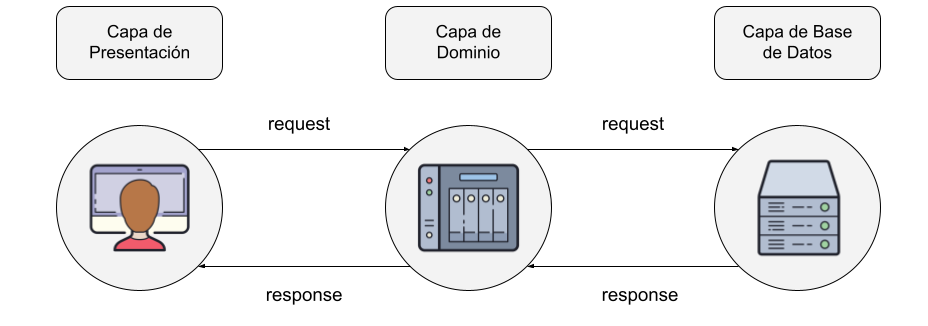
\includegraphics[width=1.03\textwidth]{gfx/Diagrama-arquitectura.png}
    \caption[Diagrama conceptual de la arquitectura]{Diagrama conceptual de la arquitectura.}\label{gfx:Diagrama-arquitectura}
\end{figure}

\section{Capa de Base de Datos}
La capa de base de datos se encarga de las operaciones de los propios datos de la aplicación. Esta capa es invisible para el usuario, ya que su funcionamiento no le incumbe. En esta capa residen los datos y además se acceden a los mismos, mediante solicitudes de almacenamiento o recuperación de información desde la capa de dominio o negocio. Comúnmente esta capa suele pertenecer a la parte Back-end del sistema.

\vspace{0.3cm}

Al tener planteado el \textit{Sprint Backlog} es importante estudiar y analizar las herramientas que compondrán la estructuración de esta capa. Incluso aunque se haya dado ligeras pinceladas de un estudio técnico (\ref{sub:estudio-competitivo-tecnico}), sigue siendo crucial reiterar y volver a incidir en este apartado antes de adentrarse en el diseño de dicha capa.

\subsection{Estudio técnico}
Los dos grandes pilares o modelos que existen actualmente en las bases de datos son denominados SQL (base de datos relacional) y NoSQL (base de datos no relacional). La principal diferencia es que NoSQl no requiere una estructura sólida y definida para trabajar con los datos, lo cual para nuestra aplicación es conveniente ya que requiere de flexibilidad a la hora de operar datos, debido a que estos cambian y se actualizan en un determinado intervalo de tiempo.

\vspace{0.3cm}

Se ha elegido MongoDB como el sistema de base de datos NoSQL, el cual es orientado a documentos y de código abierto. Es de los sistemas más fiables que existen actualmente, además de su conveniencia por ser orientado a objetos, simple, dinámico y escalable. \cite{mongodb-manual}

\vspace{0.3cm}

Se ha elegido el lenguaje Python principalmente por el estudio que se realizó anteriormente en la sección \ref{sub:estudio-competitivo-tecnico}, debido al peso que suponían ambas librerías. Por lo que se ha decidido continuar usando dicho lenguaje y adaptar la base de datos. Pese a que este lenguaje no ha demostrado ser el más eficiente, sigue siendo muy versátil a la hora de trabajar. Con esto, se han seguido las buenas prácticas y se ha usado el \textit{driver} oficial de MongoDB, llamado PyMongo, consiguiendo de manera nativa poder almacenar datos en documentos tipo JSON. Además, Python tiene extensas bibliotecas que procesan directamente los formatos de datos de tipo JSON y BSON. \cite{mongodb-manual}

\vspace{0.3cm}

En cuanto a la plataforma como servicio que se ha elegido en este caso será MongoDB Atlas. Esto debido a que posee un plan gratuito, aunque con muchas limitaciones. La base de datos en la nube funcionaria de la misma manera que en la versión local, pero teniendo en cuenta las limitaciones técnicas.

\vspace{0.3cm}

\begin{figure}[H]
    \centering
    \myfloatalign
    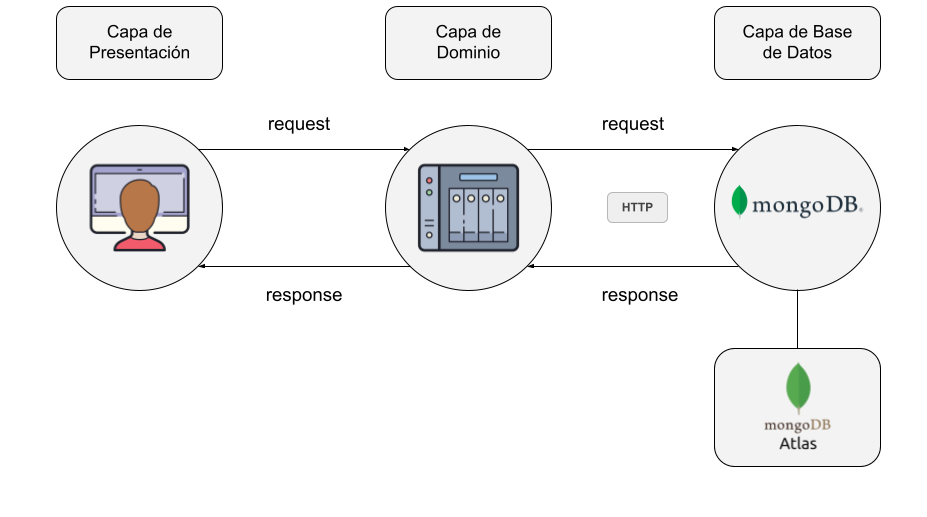
\includegraphics[width=1\textwidth]{gfx/DiagramaRutas1.png}
    \caption[Diagrama conceptual con más detalle (1)]{Diagrama conceptual de la arquitectura, con la Capa de Base de Datos detallada.}\label{gfx:DiagramaRutas1}
\end{figure}

\subsection{Modelado de datos}
El modelo de datos principal será compuesto por dos clases. Las dos clases harán referencia al mismo modelo pero tendrán dos conceptos diferentes, uno para objetos nuevos y otro para su actualización. De esta manera tenemos dos clases, las cuales se llaman \textit{Country} y \textit{CountryUpdate}. La diferencia es que la primera clase creará un id nuevo para cada objeto y la segunda no.

\vspace{0.3cm}

Ambas poseen los mismo atributos y entidades. Están formadas por país y fecha, como los parámetros principales para poder clasificar el objeto y buscarlo en la base de datos. Luego está la lista de diferentes tendencias, la cual se va actualizando a lo largo del día.

\vspace{0.3cm}

Muchos de los atributos pueden llegar a ser opcionales, como por ejemplo la imagen del articulo, la cual si no existe se cargará otra por defecto desde la interfaz. En el siguiente diagrama se puede visualizar el conjunto del modelado, aunque las diferentes entidades serán explicadas en la capa de dominio o negocio.

\vspace{0.3cm}

\begin{figure}[H]
    \centering
    \myfloatalign
    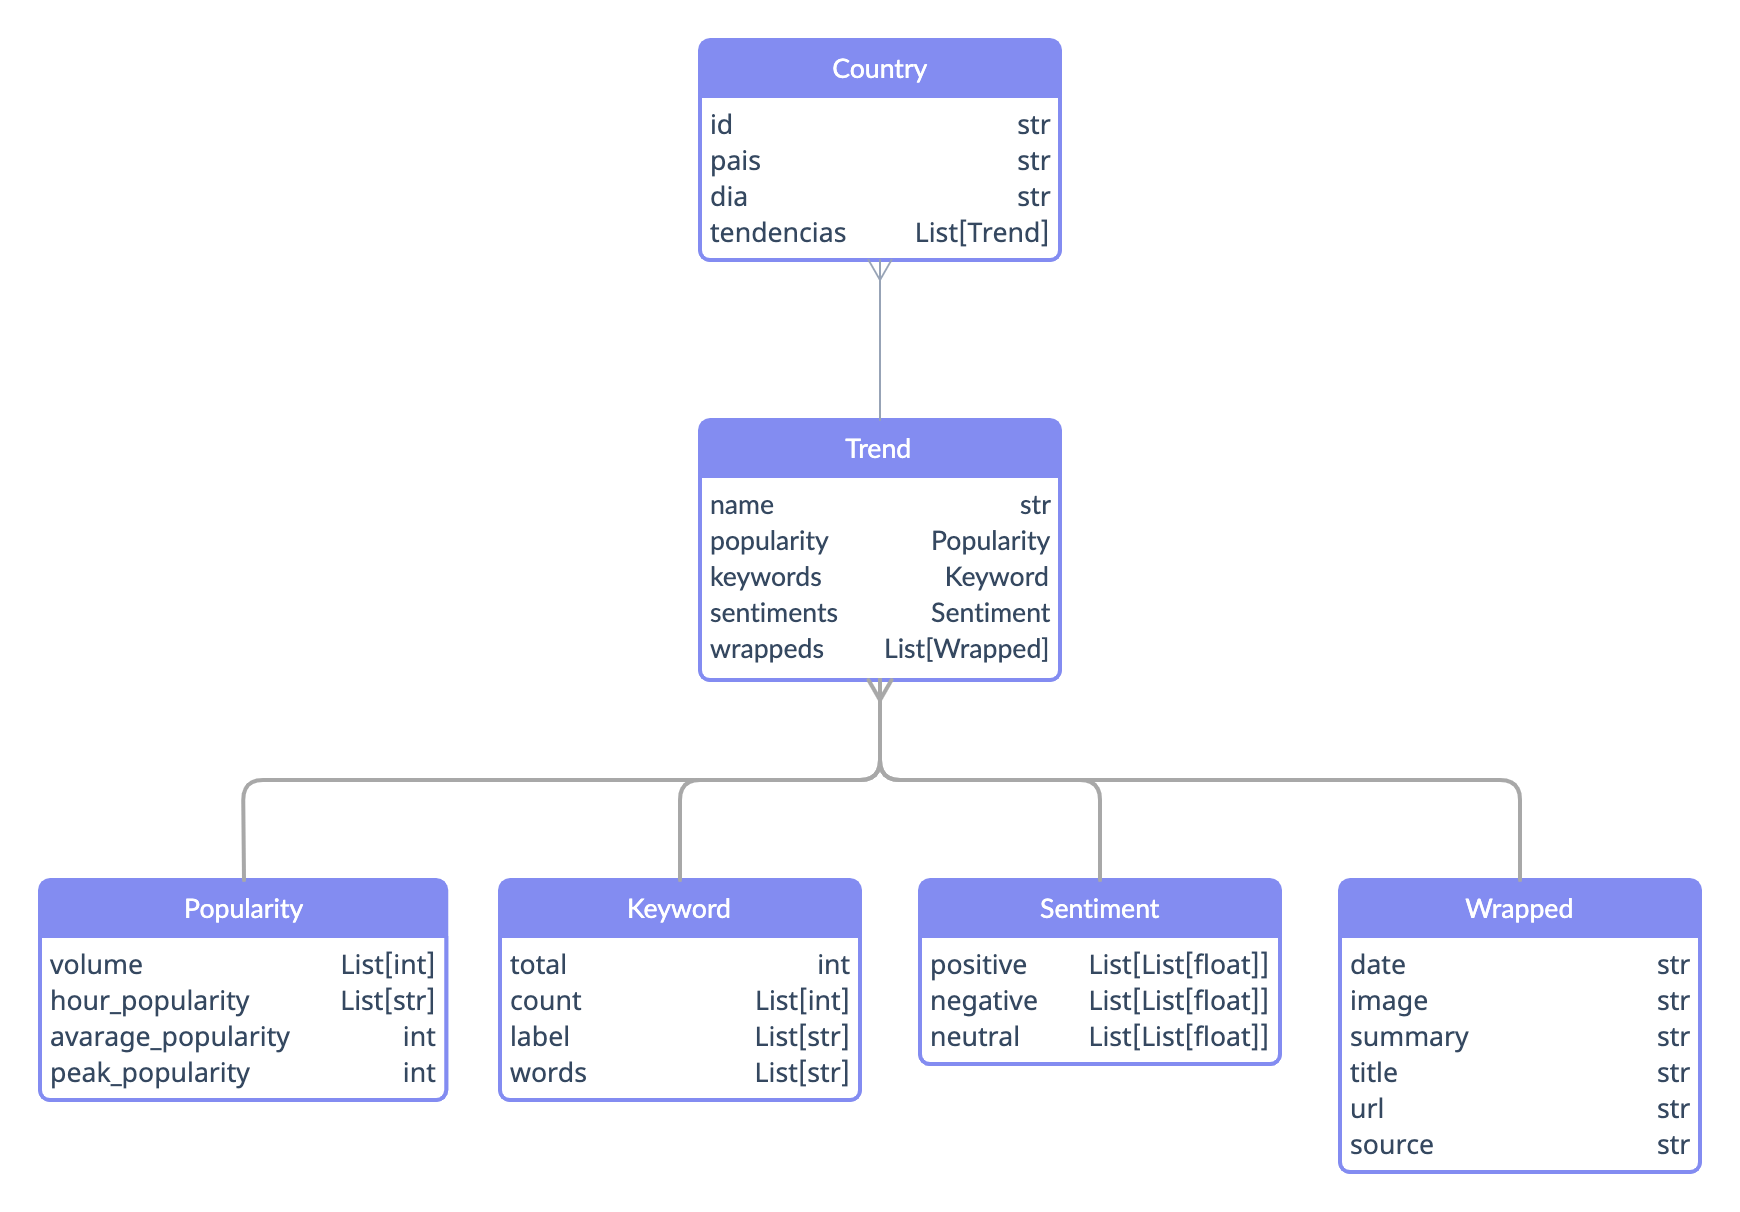
\includegraphics[width=1\textwidth]{gfx/Models-diagram.png}
    \caption[Diagrama de relación de la base de datos]{Diagrama de relación de la base de datos.}\label{gfx:Models-diagram}
\end{figure}

\newpage

\subsubsection{Entidad Tendencia}\label{subsub:ent-tendencia}
Esta entidad representa el modelado de datos de las historias de usuario cubiertas en el Sprint 2 (\ref{subs:sprint-2}). En ellas el usuario debe poder visualizar datos de diez tendencias como máximo.
\begin{figure}[H]
    \centering
    \myfloatalign
    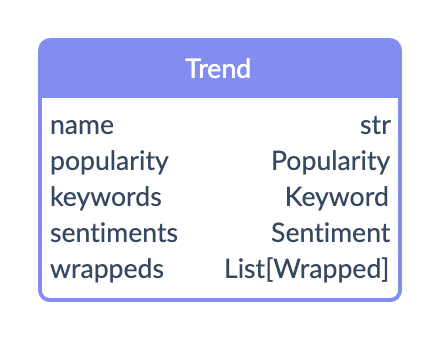
\includegraphics[width=0.4\textwidth]{gfx/diagrama-er0.png}
    \caption[Diagrama de relación de Tendencia]{Diagrama de relación de Tendencia.}\label{gfx:diagrama-er0}
\end{figure}
Para poder representar debidamente la historia de usuario se debe ir calculando progresivamente los siguientes valores:
\\\\
\textit{name}: el nombre de la tendencia.  \\
\textit{popularity}: el objeto popularidad de la tendencia.    \\
\textit{keywords}: el objeto \textit{keywords} de la tendencia.    \\
\textit{sentiments}: el objeto sentimientos general de la tendencia.    \\
\textit{wrappeds}: lista de objetos noticia de la tendencia.

\subsubsection{Entidad Popularidad}\label{subsub:ent-popularidad}
Esta entidad representa el modelado de datos de las historias de usuario cubiertas en el Sprint 6 (\ref{subs:sprint-6}). En ellas el usuario debe poder visualizar datos de interés sobre la popularidad y también una gráfica de área.
\begin{figure}[H]
    \centering
    \myfloatalign
    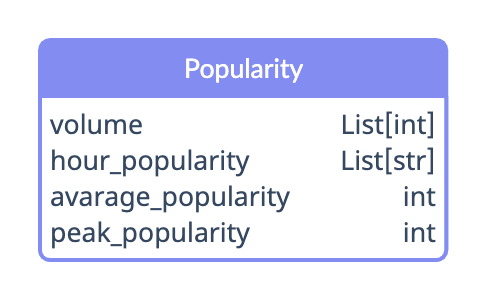
\includegraphics[width=0.4\textwidth]{gfx/diagrama-er1.png}
    \caption[Diagrama de relación de Popularidad]{Diagrama de relación de Popularidad.}\label{gfx:diagrama-er1}
\end{figure}

Para poder representar debidamente las H.U. se debe ir calculando progresivamente los siguientes valores:
\\\\
\textit{volume}: el volumen de popularidad que está teniendo la tendencia.  \\
\textit{hour\_popularity}: la hora en la que fue registrada el volumen.    \\
\textit{avarage\_popularity}: popularidad media de la tendencia.    \\
\textit{peak\_popularity}: popularidad más alta de la tendencia.

\subsubsection{Entidad Palabras más Comunes y Keywords}\label{subsub:ent-keywords}
Esta entidad representa el modelado de datos las historias de usuario cubiertas en el Sprint 7 (\ref{subs:sprint-7}). En ellas el usuario debe poder visualizar datos de interés sobre las palabras más comunes, las \textit{keywords} y una gráfica de radial de barras correspondiente.
\begin{figure}[H]
    \centering
    \myfloatalign
    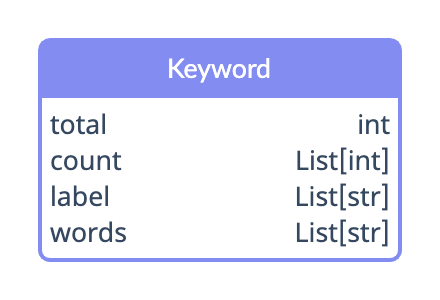
\includegraphics[width=0.4\textwidth]{gfx/diagrama-er2.png}
    \caption[Diagrama de relación de Palabras más Comunes y Keywords]{Diagrama de relación de Palabras más Comunes y Keywords.}\label{gfx:diagrama-er2}
\end{figure}

Para poder representar debidamente las H.U. se debe ir calculando progresivamente los siguientes valores:
\\\\
\textit{total}: el volumen de publicaciones recogidas de la tendencia.  \\
\textit{count}: las repeticiones de palabras comunes.    \\
\textit{label}: las palabras comunes en cuestión.    \\
\textit{words}: las \textit{keywords} extraídas.

\subsubsection{Entidad Sentimiento General}\label{subsub:ent-sentiment}
Esta entidad representa el modelado de datos de las historias de usuario cubiertas en el Sprint 8 (\ref{subs:sprint-8}). En ellas el usuario debe poder visualizar datos de interés sobre el sentimiento general de los tweets o publicaciones y una gráfica de burbujas correspondiente.
\begin{figure}[H]
    \centering
    \myfloatalign
    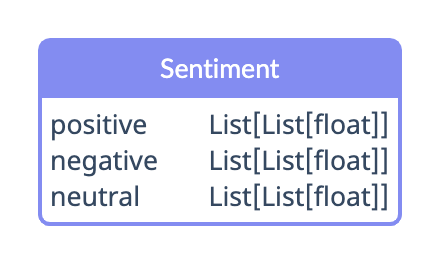
\includegraphics[width=0.4\textwidth]{gfx/diagrama-er3.png}
    \caption[Diagrama de relación de Sentimiento General]{Diagrama de relación de Sentimiento General.}\label{gfx:diagrama-er3}
\end{figure}

Para poder representar debidamente las H.U. se debe ir calculando progresivamente los siguientes valores:
\\\\
\textit{positive}: datos sobre el sentimiento positivo.  \\
\textit{negative}: datos sobre el sentimiento negativo.    \\
\textit{neural}: datos sobre el sentimiento neutro.

\subsubsection{Entidad Noticas Relacionadas}\label{subsub:ent-noticias}
Esta entidad representa el modelado de datos las historias de usuario cubiertas en el Sprint 9 (\ref{subs:sprint-9}). En ellas el usuario debe poder visualizar datos de interés sobre las noticias o artículos relacionados sobre la tendencia.
\begin{figure}[H]
    \centering
    \myfloatalign
    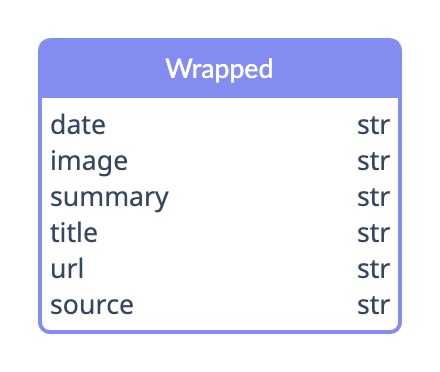
\includegraphics[width=0.4\textwidth]{gfx/diagrama-er4.png}
    \caption[Diagrama de relación de Noticas Relacionadas]{Diagrama de relación de Noticas Relacionadas.}\label{gfx:diagrama-er4}
\end{figure}

Para poder representar debidamente la H.U. se debe ir calculando progresivamente los siguientes valores:
\\\\
\textit{date}: fecha de publicación de la noticia.  \\
\textit{image}: imagen relacionada de la noticia.    \\
\textit{summary}: texto relacionado de la noticia.    \\
\textit{title}: titulo de la noticia.    \\
\textit{url}: enlace de la noticia.    \\
\textit{source}: editorial de la noticia.

\section{Capa de Dominio o Negocio}
La capa de dominio o negocio permite la interacción entre la capa de base de datos y la capa de presentación. Es la capa encargada de gestionar tanto las distintas peticiones recibidas desde la capa de presentación, como los datos almacenados en la capa de base de datos. Comúnmente esta capa suele pertenecer a la parte Back-end del sistema.

\subsection{Estudio técnico}
Al plantear la aplicación en la capa de dominio o negocio, surgen ciertas pautas o normativas que conviene seguir. Surge la denominación \ac{API} para las interacciones que surgen entre la capa de presentación y la capa actual. Otra denominación que conviene saber es \ac{REST}, el cual es un conjunto de limites a la hora de implementar una \ac{API}. \cite{redahat-manual}

\vspace{0.3cm}

Cuando un usuario envía una petición a través de una API REST o RESTful, esta transfiere una representación del estado del recurso solicitado al solicitante o al extremo. Generalmente la información se envía a través de \ac{HTTP} en formato \ac{JSON}, un lenguaje popular y fácilmente entendible. \cite{redahat-manual}

\vspace{0.3cm}

La mayoría de las interacciones se pueden resumir en el nemónico de las cuatro funciones del almacenamiento persistente llamado \ac{CRUD}. Las funciones \ac{CRUD} implican el uso de las operaciones \ac{HTTP}, las cuales son PUT, GET, POST, DELETE o PATCH.

\vspace{0.3cm}

Habiendo definido propiamente las pautas de una \ac{API} \ac{REST}, podemos proceder a elegir el \textit{microframework} que cumpla y revele las operaciones salientes mediante la interfaz \ac{REST} y \textit{websockets}. Para ello se ha elegido de nuevo el lenguaje Python, debido a que exista compatibilidad entre la capa de base de datos y la de dominio o negocio y además por su versatilidad a la hora de trabajar con diferentes librerías que  serán extremadamente útiles para la realización de diversas historias de usuario.

\vspace{0.3cm}

Actualmente, en Python existen \textit{frameworks} que funcionan con el estándar \ac{WSGI} o \ac{ASGI}. El último mencionado es el más actual y utiliza corrutinas introducidas en las versiones más recientes de Python, lo que mejora el uso de la CPU en servidores web intensivos de E/S.

\vspace{0.3cm}

Las principales implementaciones de servidor \ac{ASGI} existentes actuales son Uvicorn, Hypercorn y Daphne. Los tres son fácilmente implementables, pero el más estable es Uvicorn, además usa una implementación escrita directamente en el lenguaje C, lo cual lo vuelve más rápido y eficiente. \cite{uvicorn-manual}

\vspace{0.3cm}

Tras haber elegido el servidor, podemos continuar con el \textit{microframework}. Actualmente existe una cantidad variada de ellos, como FastAPI, Starlette o Django, pero finalmente me he decantado por la primera opción. FastAPI es mucho más ligero que Django y además funciona de una manera parecida a Starlette, pero le añade funcionalidades como validación o documentación. \cite{fastapi-manual}

\vspace{0.3cm}

La implementación de las rutas fue realizada con el objeto \textit{router}, el cual tiene la función de declarar todas las rutas con decoradores y añadir el prefijo que llevaran dichas rutas. Posteriormente se crea la documentación automática.

\vspace{0.3cm}

\begin{figure}[H]
    \centering
    \myfloatalign
    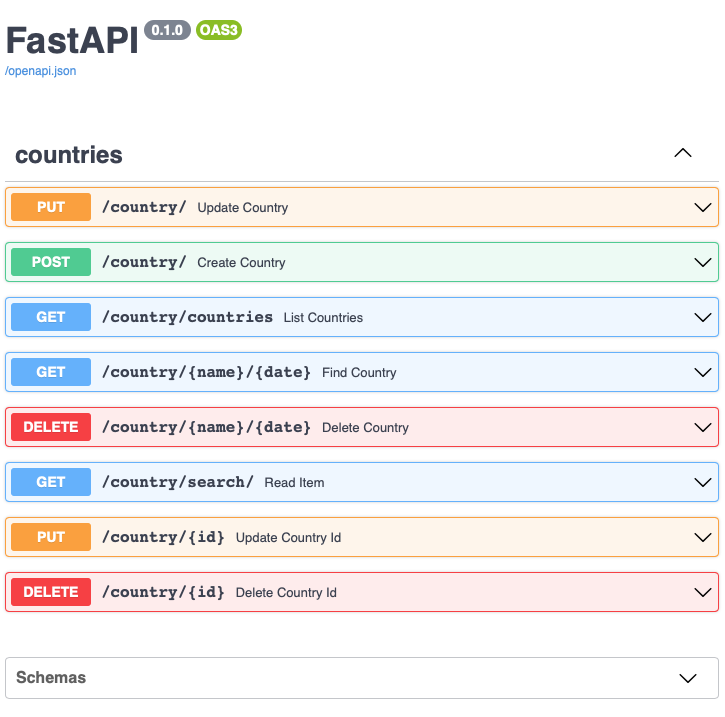
\includegraphics[width=1\textwidth]{gfx/fastapi-rutas.png}
    \caption[Documentación generada por FastAPI]{Documentación generada por FastAPI.}\label{gfx:fastapi-rutas}
\end{figure}

En cuanto a la plataforma como servicio (\ac{PaaS}) he elegido Heroku, la cual tiene opciones gratuitas y está basada en contenedores. La gran ventaja de Heroku, aparte de tener un plan gratuito, es que tiene múltiple soporte de lenguajes y entre ellos Python. Las rutas declaradas y la de por defecto funcionarían de la misma manera que localmente. \cite{heroku-manual}

\vspace{0.3cm}

Además otra ventaja crucial, la cual es requerida para el correcto funcionamiento de la aplicación, es que un proceso se ejecute cada determinado intervalo de tiempo. Esto es debido a que necesitamos que se actualice la información de las tendencias, por lo que localmente tendríamos que configurar un \textit{cron} ejecutando un \textit{script} de Python y en Heroku tenemos un \textit{Scheduler}, el cual tiene el mismo comportamiento. Dicho proceso ha sido configurado para que se ejecute cada hora y el \textit{script} en cuestión recopilará toda la información necesaria.

\vspace{0.3cm}

\begin{figure}[H]
    \centering
    \myfloatalign
    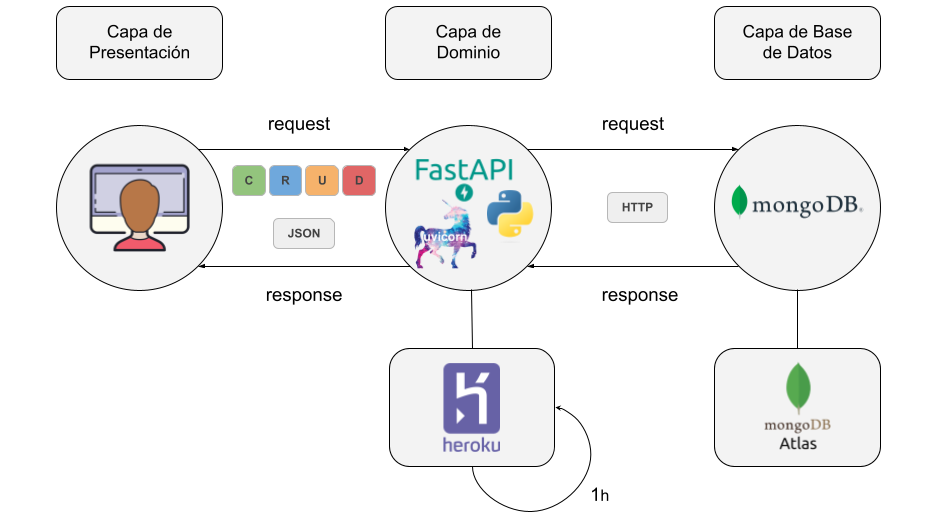
\includegraphics[width=0.91\textwidth]{gfx/DiagramaRutas2.png}
    \caption[Diagrama conceptual con más detalle (2)]{Diagrama conceptual de la arquitectura, con la Capa de Dominio o Negocio y Base de Datos detallada.}\label{gfx:DiagramaRutas2}
\end{figure}

\subsection{Diagramas de interacción de distintas rutas}

\begin{figure}[H]
    \centering
    \myfloatalign
    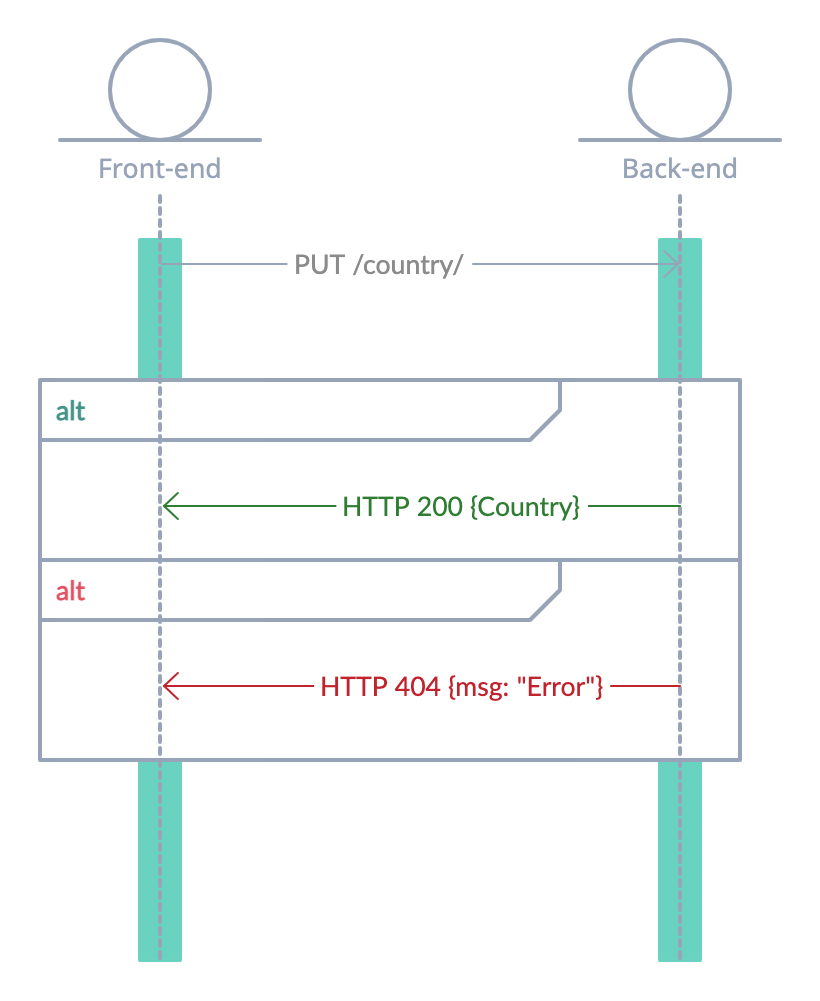
\includegraphics[width=0.39\textwidth]{gfx/diagrama-itr1.png}
    \caption[Diagrama interacción de rutas (1)]{Diagrama interacción de rutas: \textit{Actualización de Country}.}\label{gfx:diagrama-itr1}
\end{figure}

\begin{figure}[H]
    \centering
    \myfloatalign
    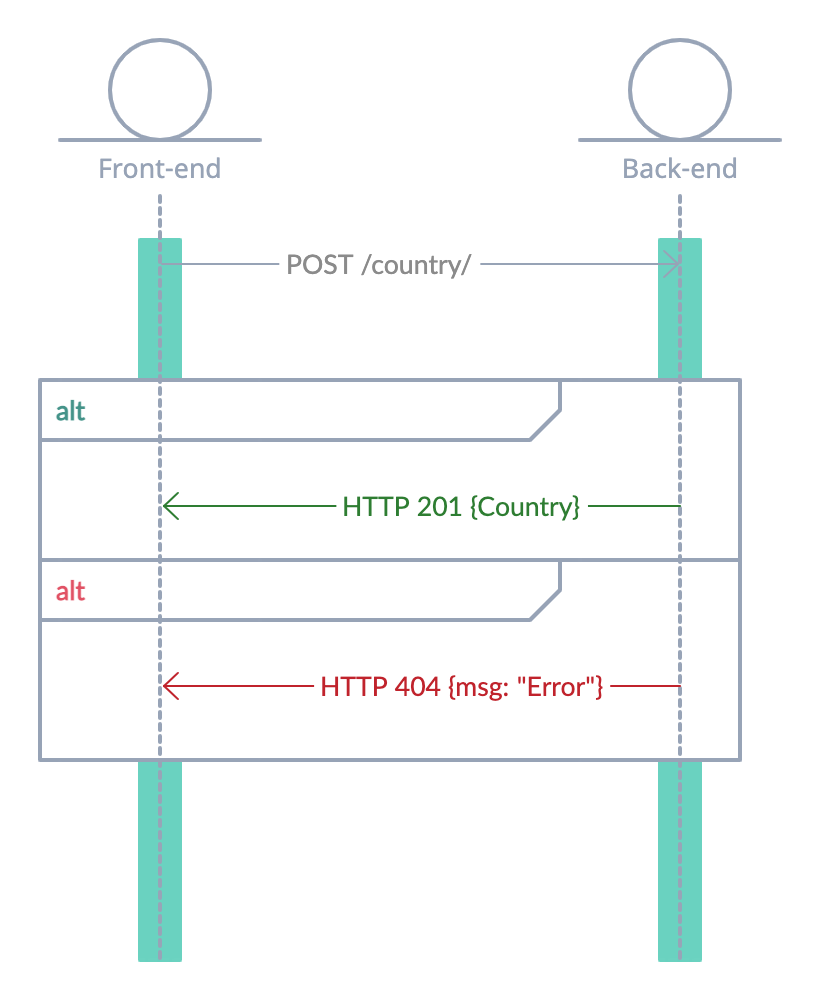
\includegraphics[width=0.39\textwidth]{gfx/diagrama-itr2.png}
    \caption[Diagrama interacción de rutas (2)]{Diagrama interacción de rutas: \textit{Creación de Country}.}\label{gfx:diagrama-itr2}
\end{figure}

\begin{figure}[H]
    \centering
    \myfloatalign
    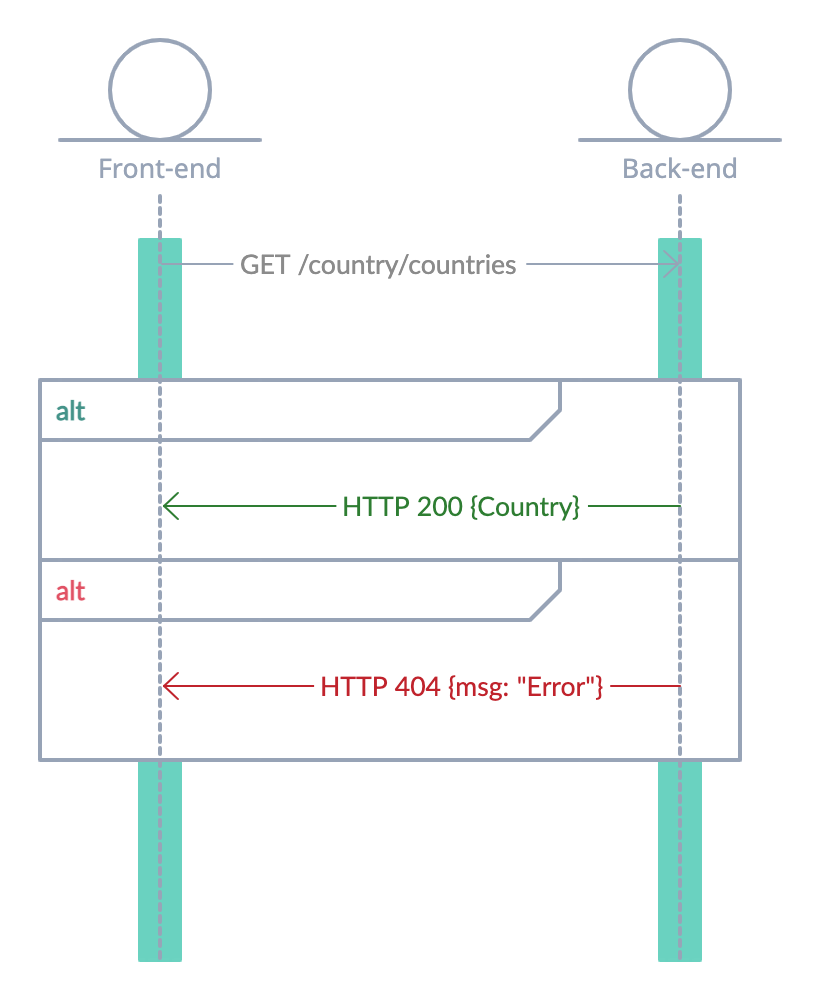
\includegraphics[width=0.44\textwidth]{gfx/diagrama-itr3.png}
    \caption[Diagrama interacción de rutas (3)]{Diagrama interacción de rutas: \textit{Lectura de lista de Country}.}\label{gfx:diagrama-itr3}
\end{figure}

\begin{figure}[H]
    \centering
    \myfloatalign
    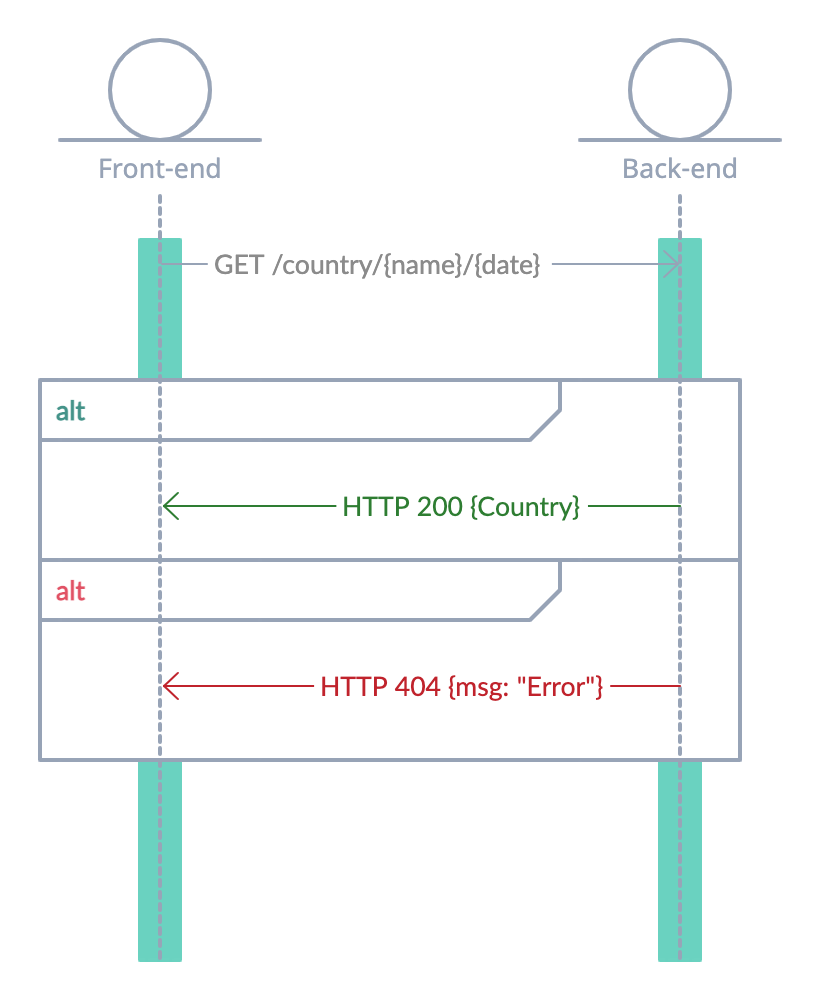
\includegraphics[width=0.44\textwidth]{gfx/diagrama-itr4.png}
    \caption[Diagrama interacción de rutas (4)]{Diagrama interacción de rutas: \textit{Lectura de Country por parámetros}.}\label{gfx:diagrama-itr4}
\end{figure}

\begin{figure}[H]
    \centering
    \myfloatalign
    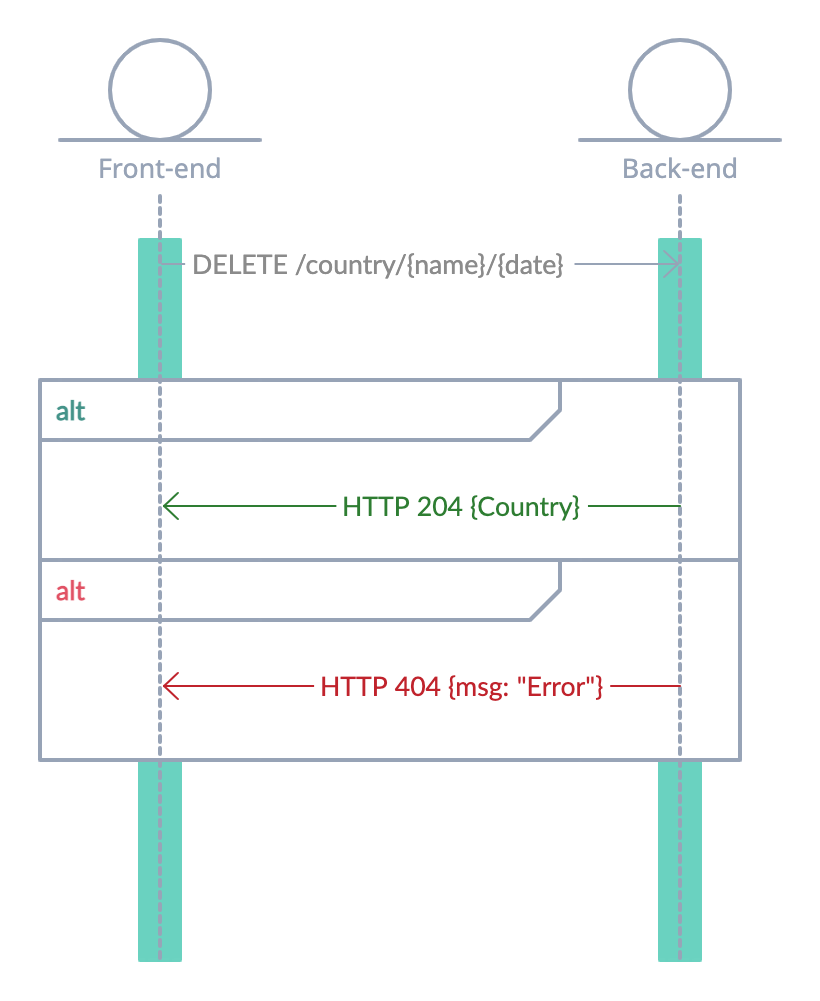
\includegraphics[width=0.44\textwidth]{gfx/diagrama-itr5.png}
    \caption[Diagrama interacción de rutas (5)]{Diagrama interacción de rutas: \textit{Eliminación de Country por parámetros}.}\label{gfx:diagrama-itr5}
\end{figure}

\begin{figure}[H]
    \centering
    \myfloatalign
    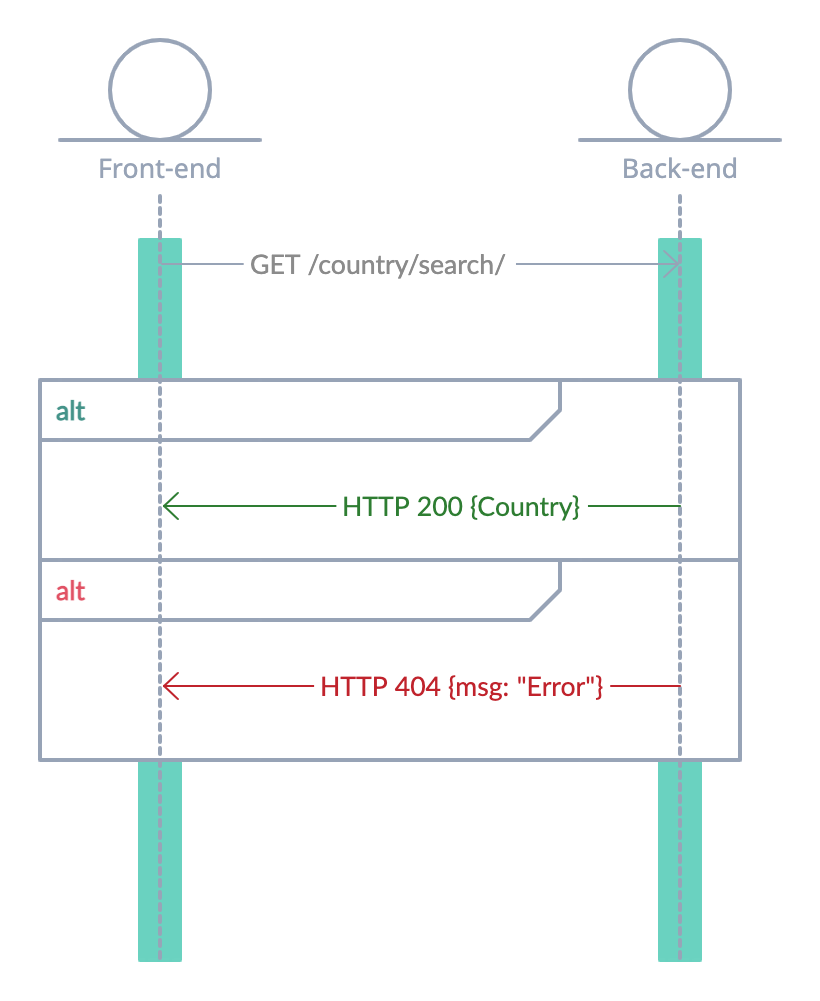
\includegraphics[width=0.45\textwidth]{gfx/diagrama-itr6.png}
    \caption[Diagrama interacción de rutas (6)]{Diagrama interacción de rutas: \textit{Lectura de la búsqueda de Country}.}\label{gfx:diagrama-itr6}
\end{figure}

\begin{figure}[H]
    \centering
    \myfloatalign
    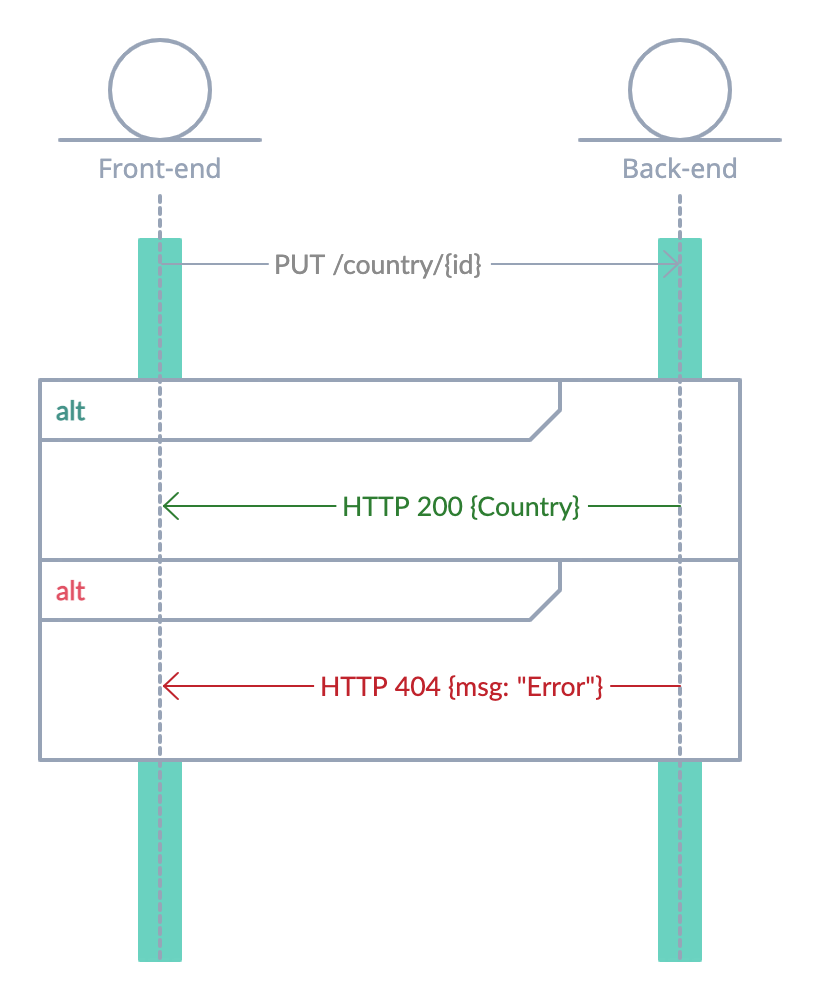
\includegraphics[width=0.45\textwidth]{gfx/diagrama-itr7.png}
    \caption[Diagrama interacción de rutas (7)]{Diagrama interacción de rutas: \textit{Actualización de Country por id}.}\label{gfx:diagrama-itr7}
\end{figure}

\begin{figure}[H]
    \centering
    \myfloatalign
    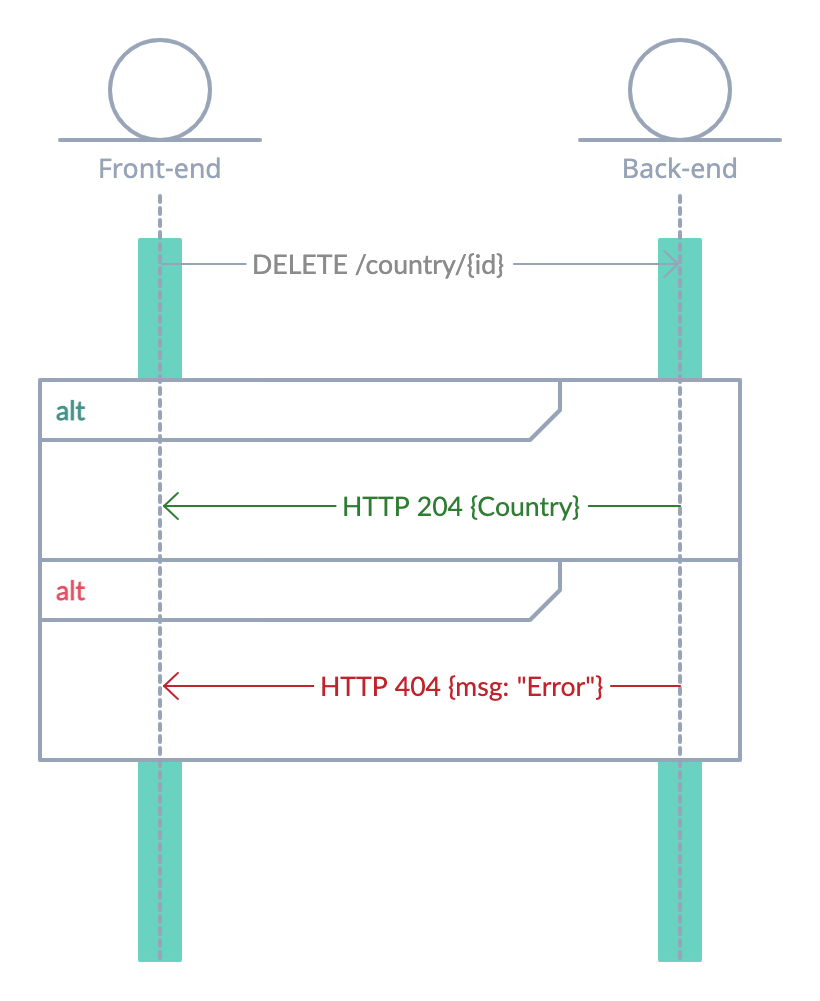
\includegraphics[width=0.45\textwidth]{gfx/diagrama-itr8.png}
    \caption[Diagrama interacción de rutas (8)]{Diagrama interacción de rutas: \textit{Eliminación de Country por id}.}\label{gfx:diagrama-itr8}
\end{figure}

\section{Capa de Presentación}
La capa de presentación se encarga de visualizar el contenido de la aplicación, donde el usuario puede interactuar directamente. De este modo esta capa será la única visible para el usuario. Comúnmente esta capa se suele denominar como Front-end.

\subsection{Estudio técnico}
Al buscar el \textit{framework} idóneo para la visualización de la aplicación surgen muchas posibilidades. Una entre ellas fue Vue, esta opción destaca por su rendimiento, escalabilidad y buena documentación. A la vez es mucho más ligera que sus competidores y además ofreciendo las mismas características, como por ejemplo el uso del \ac{DOM} virtual, el cual tiene sus ventajas a la hora de renderizar los mismos componentes de una página. En nuestro caso los componentes como las cartas se podrían beneficiar de ello. \cite{VueComparison}

\vspace{0.3cm}

Uno de los principales objetivos de la aplicación, que ya se había planteado antes, es que el contenido se pueda visualizar por medio de módulos o cartas. Por lo que al diseñar la propia aplicación, tendremos una vista principal y cada una de las cartas estará dividida en una subvista. Cada subvista tendrá sus propiedades, sus propias funciones y clases CSS. La mayoría de las clases estarán implementadas directamente a mano, menos las más básicas o convenientes ya que usaré el \textit{framework} TailwindCSS para agilizar el trabajo.

\vspace{0.3cm}

En cuanto a la plataforma como servicio (\ac{PaaS}) para la capa de presentación me he decantado por Vercel, realmente tenía mucho parecido a otras plataformas como Netlify, aunque tras usar ambas plataformas he podido concluir que Vercel funciona más eficientemente y de una manera más simple. Además posee integración con Vue, lo cual me ha permitido exportar fácilmente el proyecto.

\begin{figure}[H]
    \centering
    \myfloatalign
    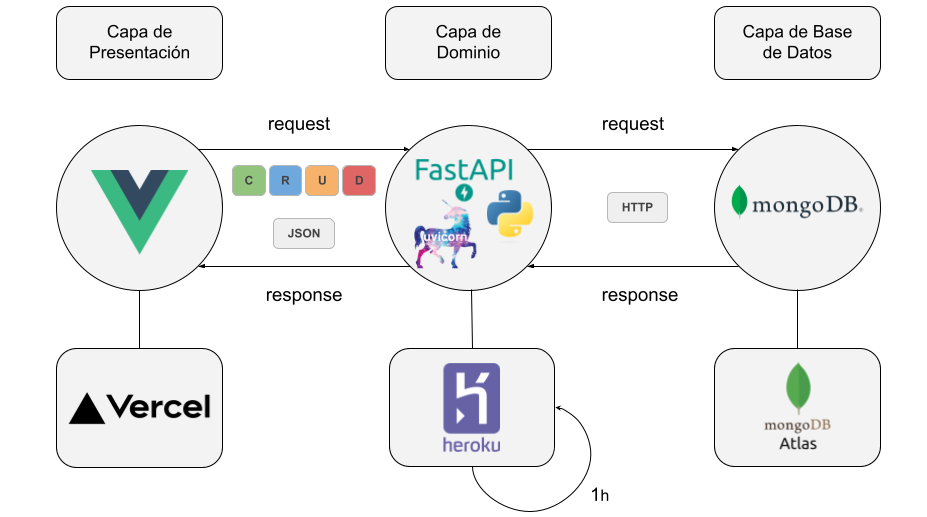
\includegraphics[width=0.83\textwidth]{gfx/DiagramaRutas3.png}
    \caption[Diagrama conceptual con más detalle (3)]{Diagrama conceptual de la arquitectura, con la Capa de Dominio o Negocio, Base de Datos y Presentación detallada.}\label{gfx:DiagramaRutas3}
\end{figure}

El contenido de la vista principal se adapta mediante parámetros y rutas. Aunque existan diferentes rutas en la capa de presentación, todas ellas devuelven la misma vista principal con los mismos componentes, a no ser que haya un error. En el siguiente diagrama se explica el funcionamiento de las distintas rutas, tanto la ruta por defecto, la ruta de la búsqueda de un tópico o la ruta por parámetros.

\begin{itemize}
    \item
    \textit{Ejemplo de ruta por defecto: \\
    https://(...)/}
    \item
    \textit{Ejemplo de ruta de búsqueda: \\
    https://(...)/search?name=Spain\&query=baloncesto}
    \item
    \textit{Ejemplo de ruta por parámetros: \\
    https://(...)/Spain/22-10-24}
\end{itemize}

\begin{figure}[H]
    \centering
    \myfloatalign
    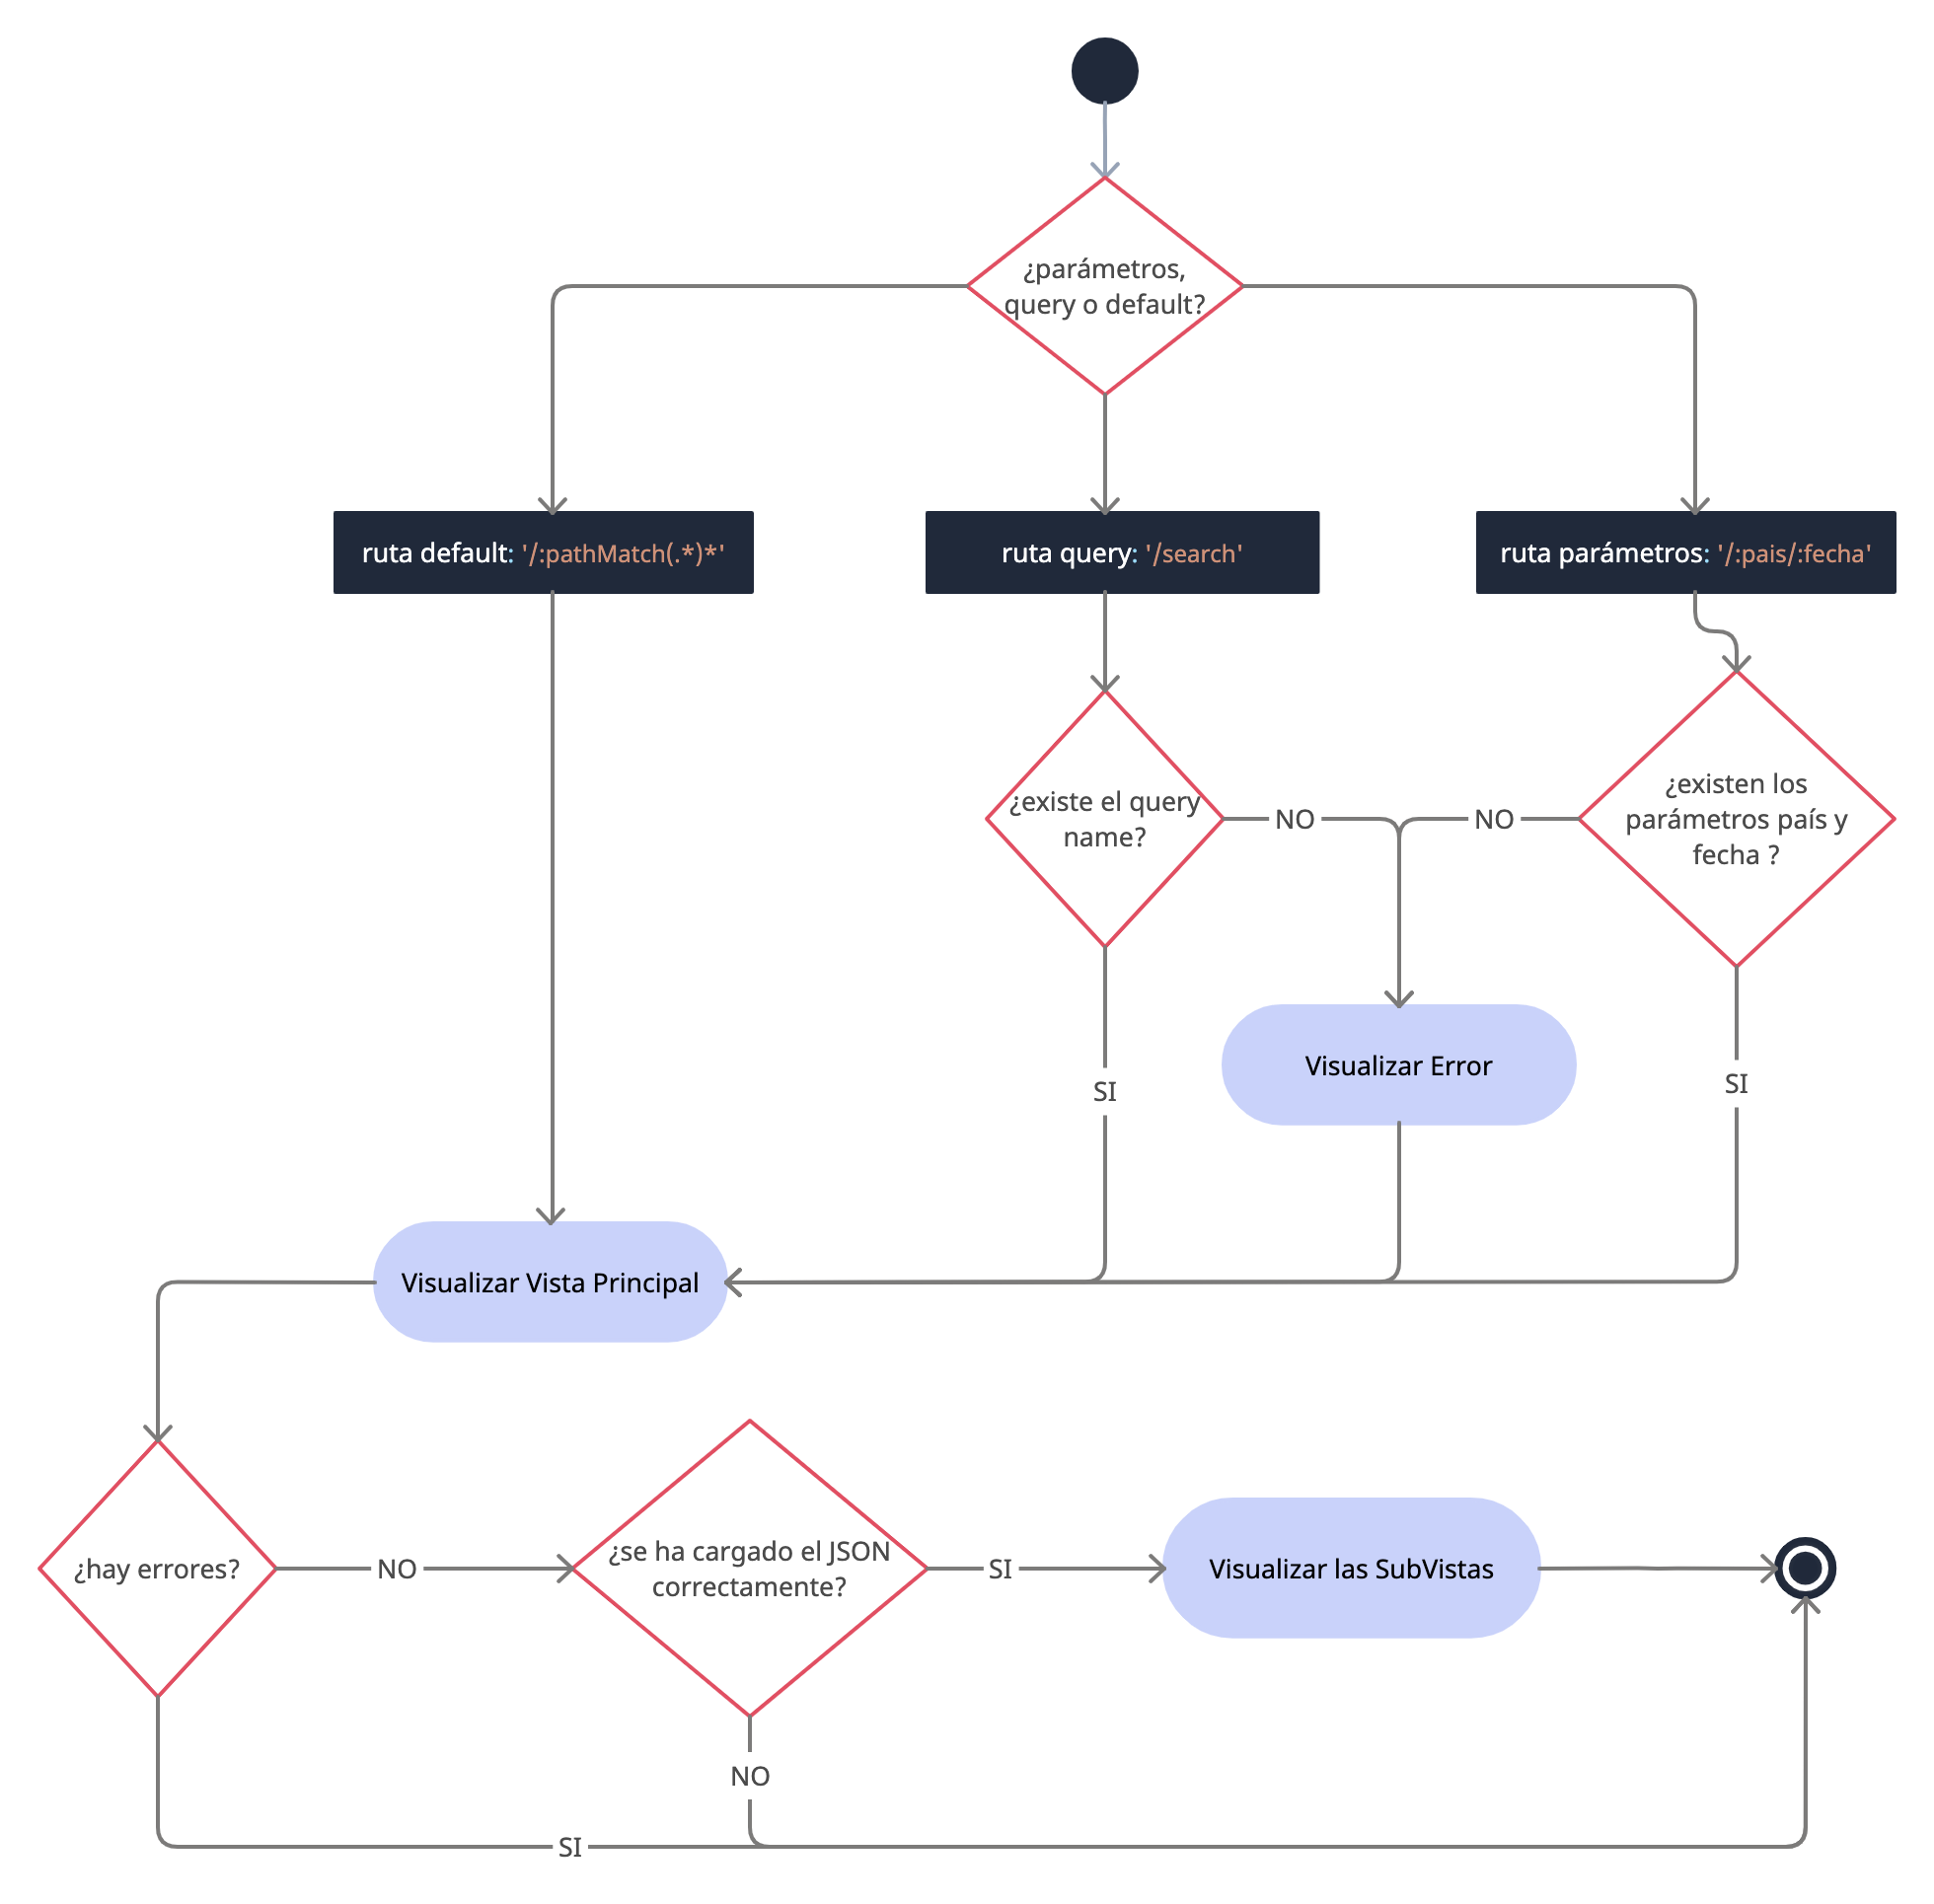
\includegraphics[width=1.001\textwidth]{gfx/Diagrama-actividad.png}
    \caption[Diagrama de actividad]{Diagrama de actividad.}\label{gfx:Diagrama-actividad}
\end{figure}

La ruta por defecto cargará como parámetro el país España y la fecha del día actual. Las demás rutas son ejecutadas al interactuar con los componentes de distintos formularios de la página. En este caso son dos, un formulario de selección (fecha y país) y otro formulario de búsqueda (los tópicos).

\vspace{0.3cm}

\begin{figure}[H]
    \centering
    \myfloatalign
    
\includegraphics[width=0.9\textwidth]{gfx/Formularios.png}
    \caption[Formularios de selección y búsqueda]{Formularios de selección y búsqueda.}\label{gfx:Formularios}
\end{figure}

Cada uno funcionan de una manera independiente, mediante eventos por click. Aunque si precisan de la información que hay en cada formulario, es decir, si el usuario cambia el parámetro país, entonces se carga una ruta con la fecha y el país seleccionado. Esto ocurre de la misma manera seleccionando la fecha o buscando un tópico, ambos necesitan la información del país seleccionado para procesar la ruta.

\subsection{Transcurso de la Interfaz de Usuario}
La vista principal es la única vista que se le llega mostrar al usuario, por lo que es importante mostrar el transcurso que ha tenido su propio diseño. Aunque como hemos explicado la vista principal se subidivide y cada subvista tiene sus propias clases de CSS, en español «Hojas de estilo en cascada». Cabe mencionar, que también se ha empleado una biblioteca que fue crucial llamada TailwindCSS.

\begin{figure}[H]
    \centering
    \myfloatalign
    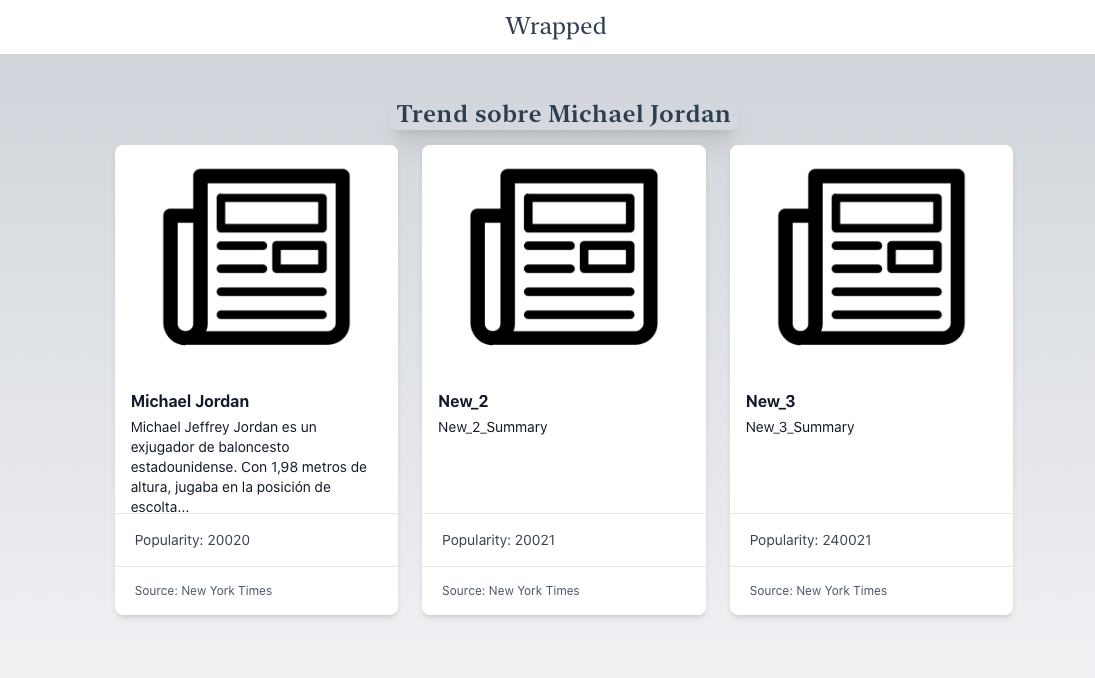
\includegraphics[width=1\textwidth]{gfx/primer-boceto.png}
    \caption[Primer boceto de la aplicación]{Primer boceto de la aplicación.}\label{gfx:primer-boceto}
\end{figure}

\begin{figure}[H]
    \centering
    \myfloatalign
    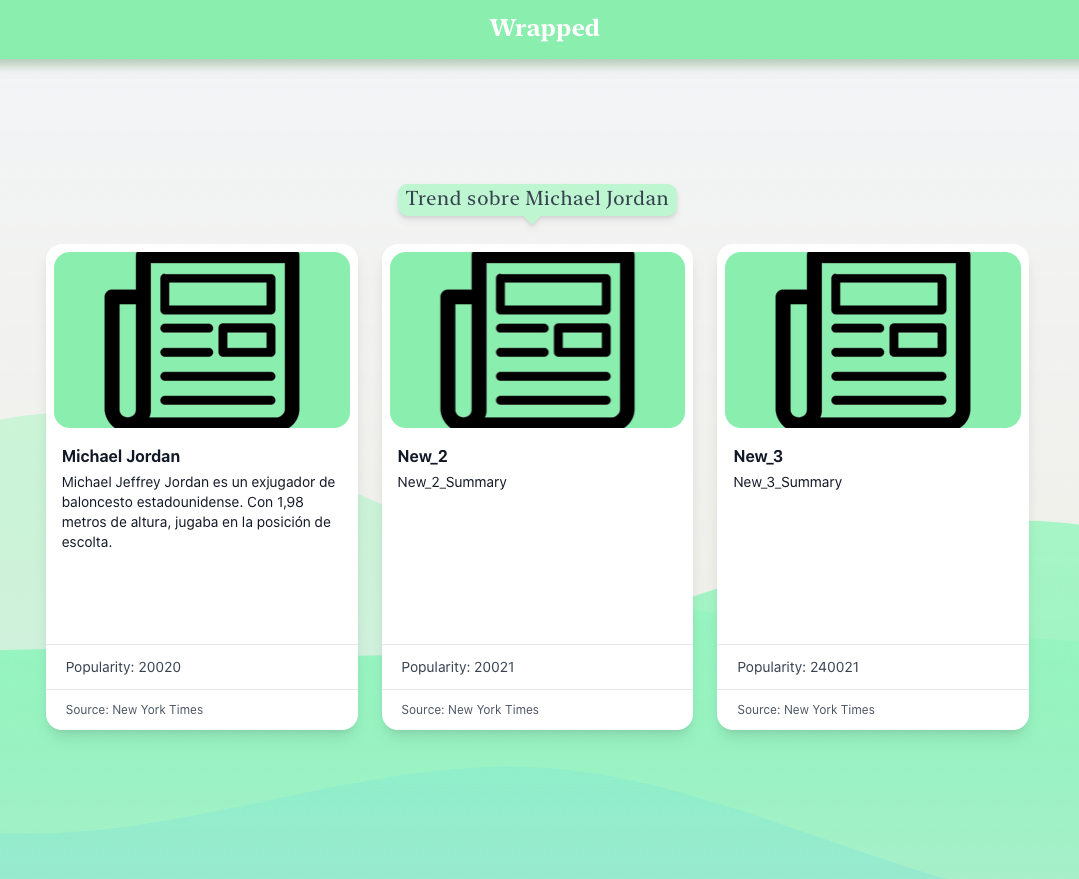
\includegraphics[width=1\textwidth]{gfx/segundo-boceto.png}
    \caption[Segundo boceto más detallado]{Segundo boceto más detallado.}\label{gfx:segundo-boceto}
\end{figure}

\begin{figure}[H]
    \centering
    \myfloatalign
    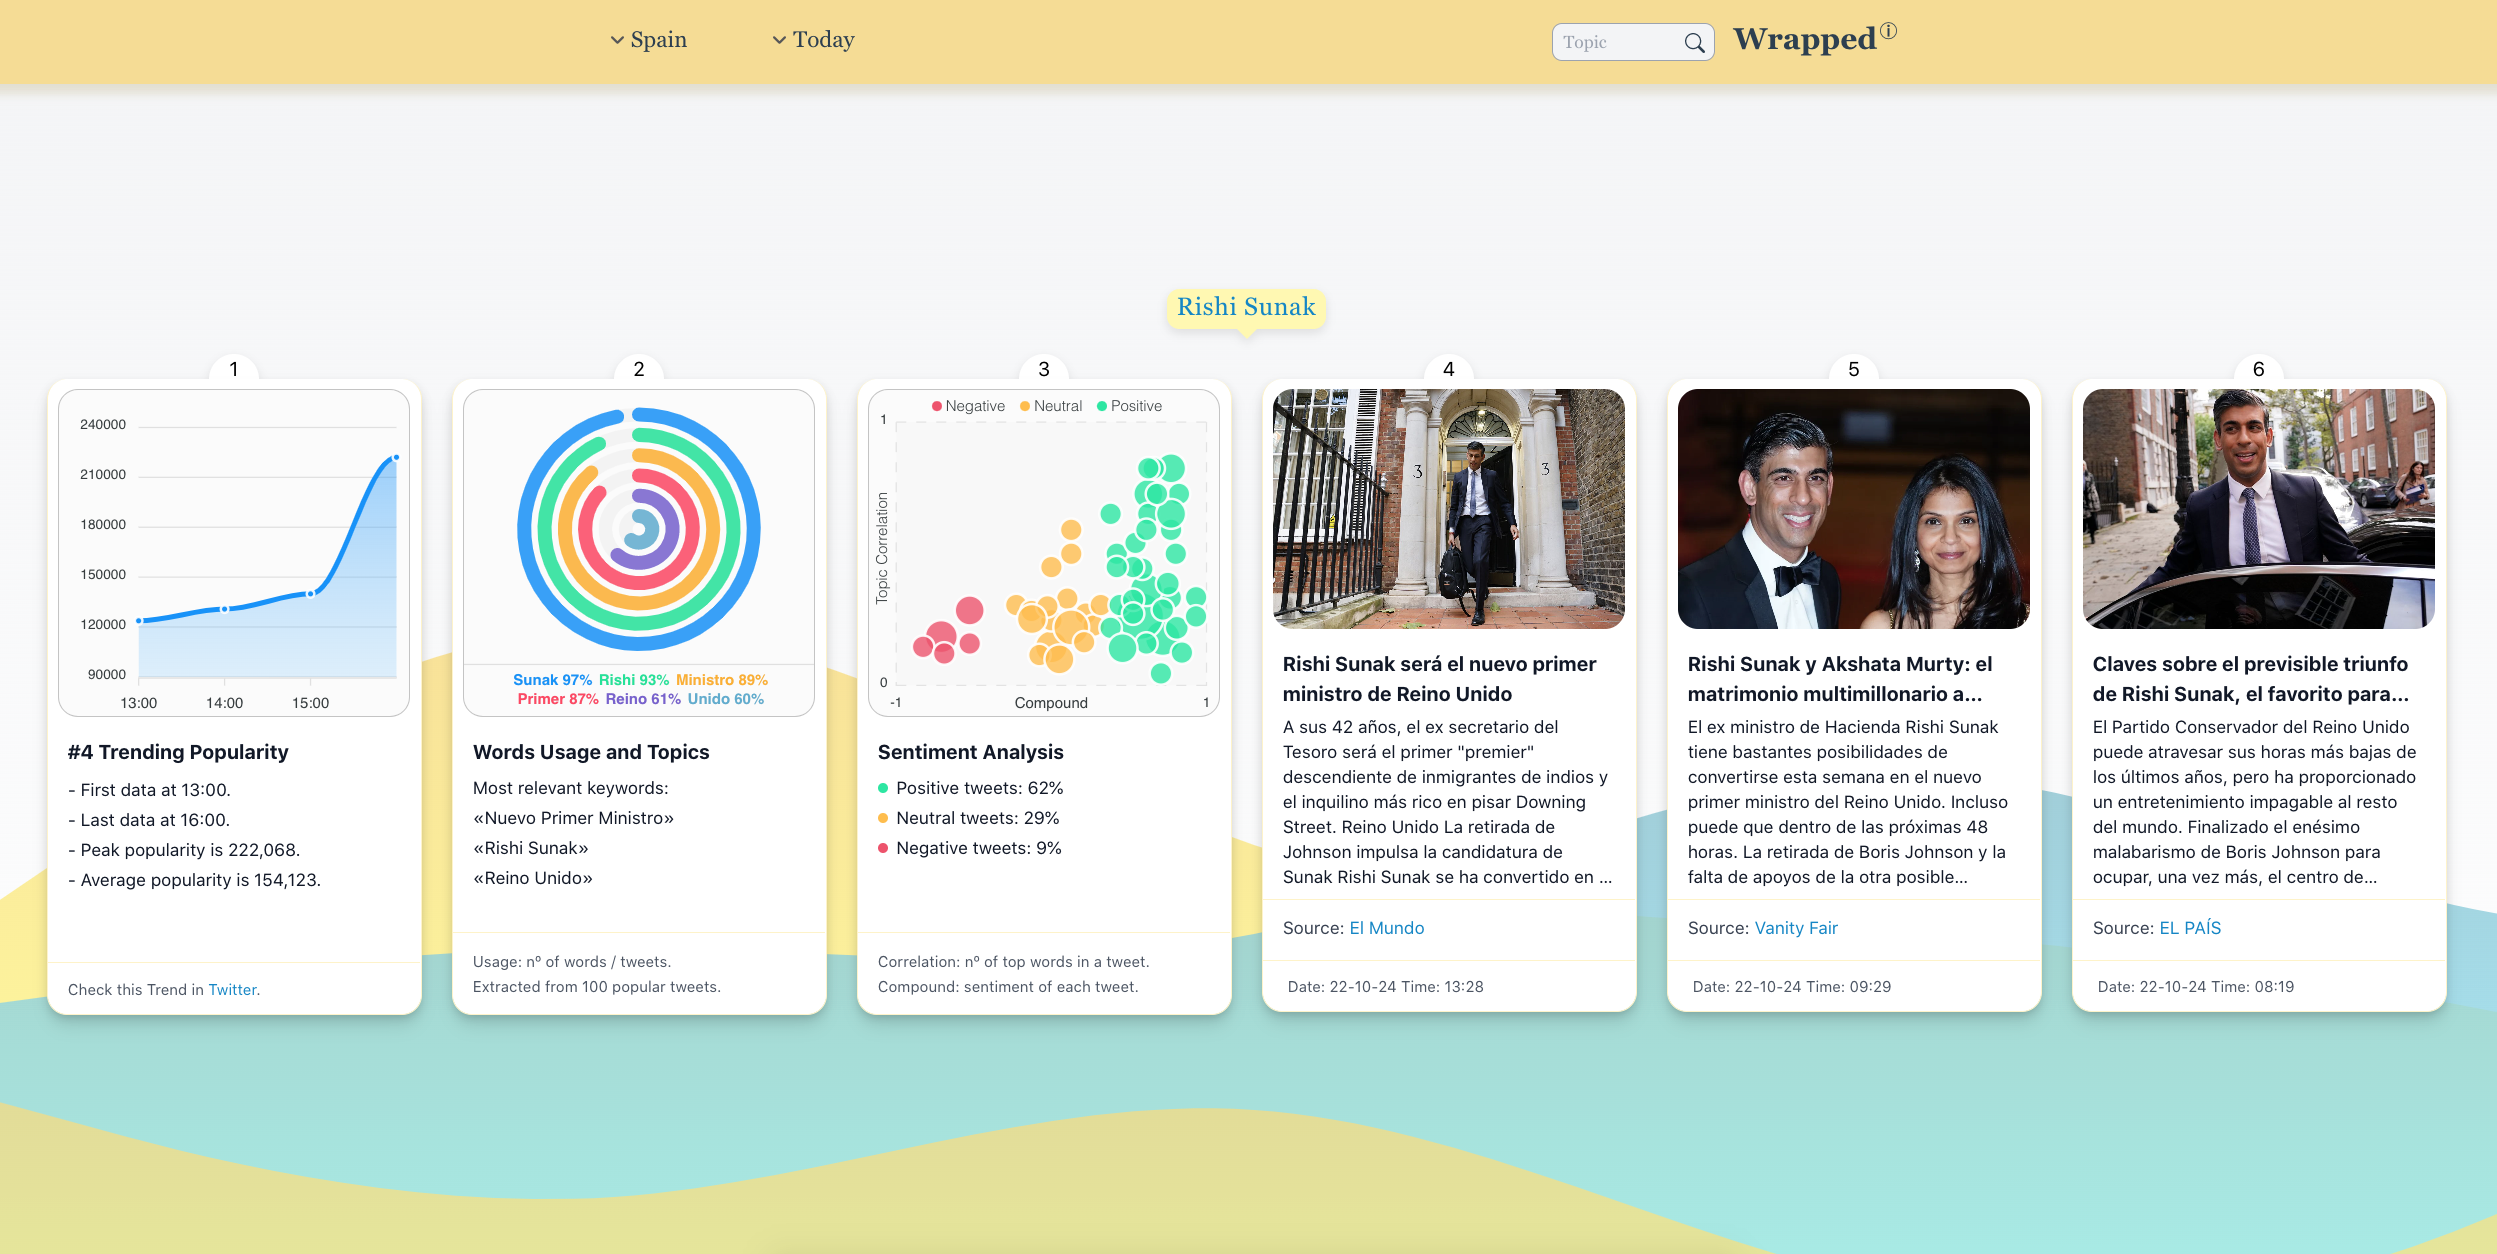
\includegraphics[width=1\textwidth]{gfx/tercer-boceto.png}
    \caption[Concepto final de la aplicación]{Concepto final de la aplicación.}\label{gfx:tercer-boceto}
\end{figure}

\begin{figure}[H]
    \centering
    \myfloatalign
    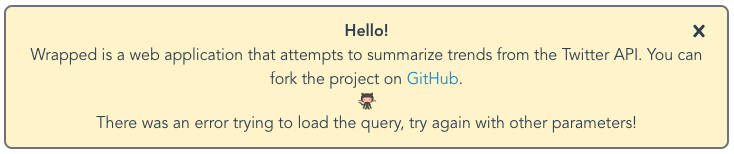
\includegraphics[width=1\textwidth]{gfx/boceto-error.png}
    \caption[Concepto del error en la visualización de parámetros]{Concepto del error en la visualización de parámetros.}\label{gfx:boceto-error}
\end{figure}

\subsection{Vista Principal}
La vista principal contiene todas las subvistas y componentes necesarios para el funcionamiento de la interfaz. Cada subvista funciona como un componente esencial dentro de la vista principal. Al cargar correctamente los datos desde la capa de dominio o negocio, estos se representan en la vista principal y a la vez cada entidad se representa con una subvista diferente.

\begin{figure}[H]
    \centering
    \myfloatalign
    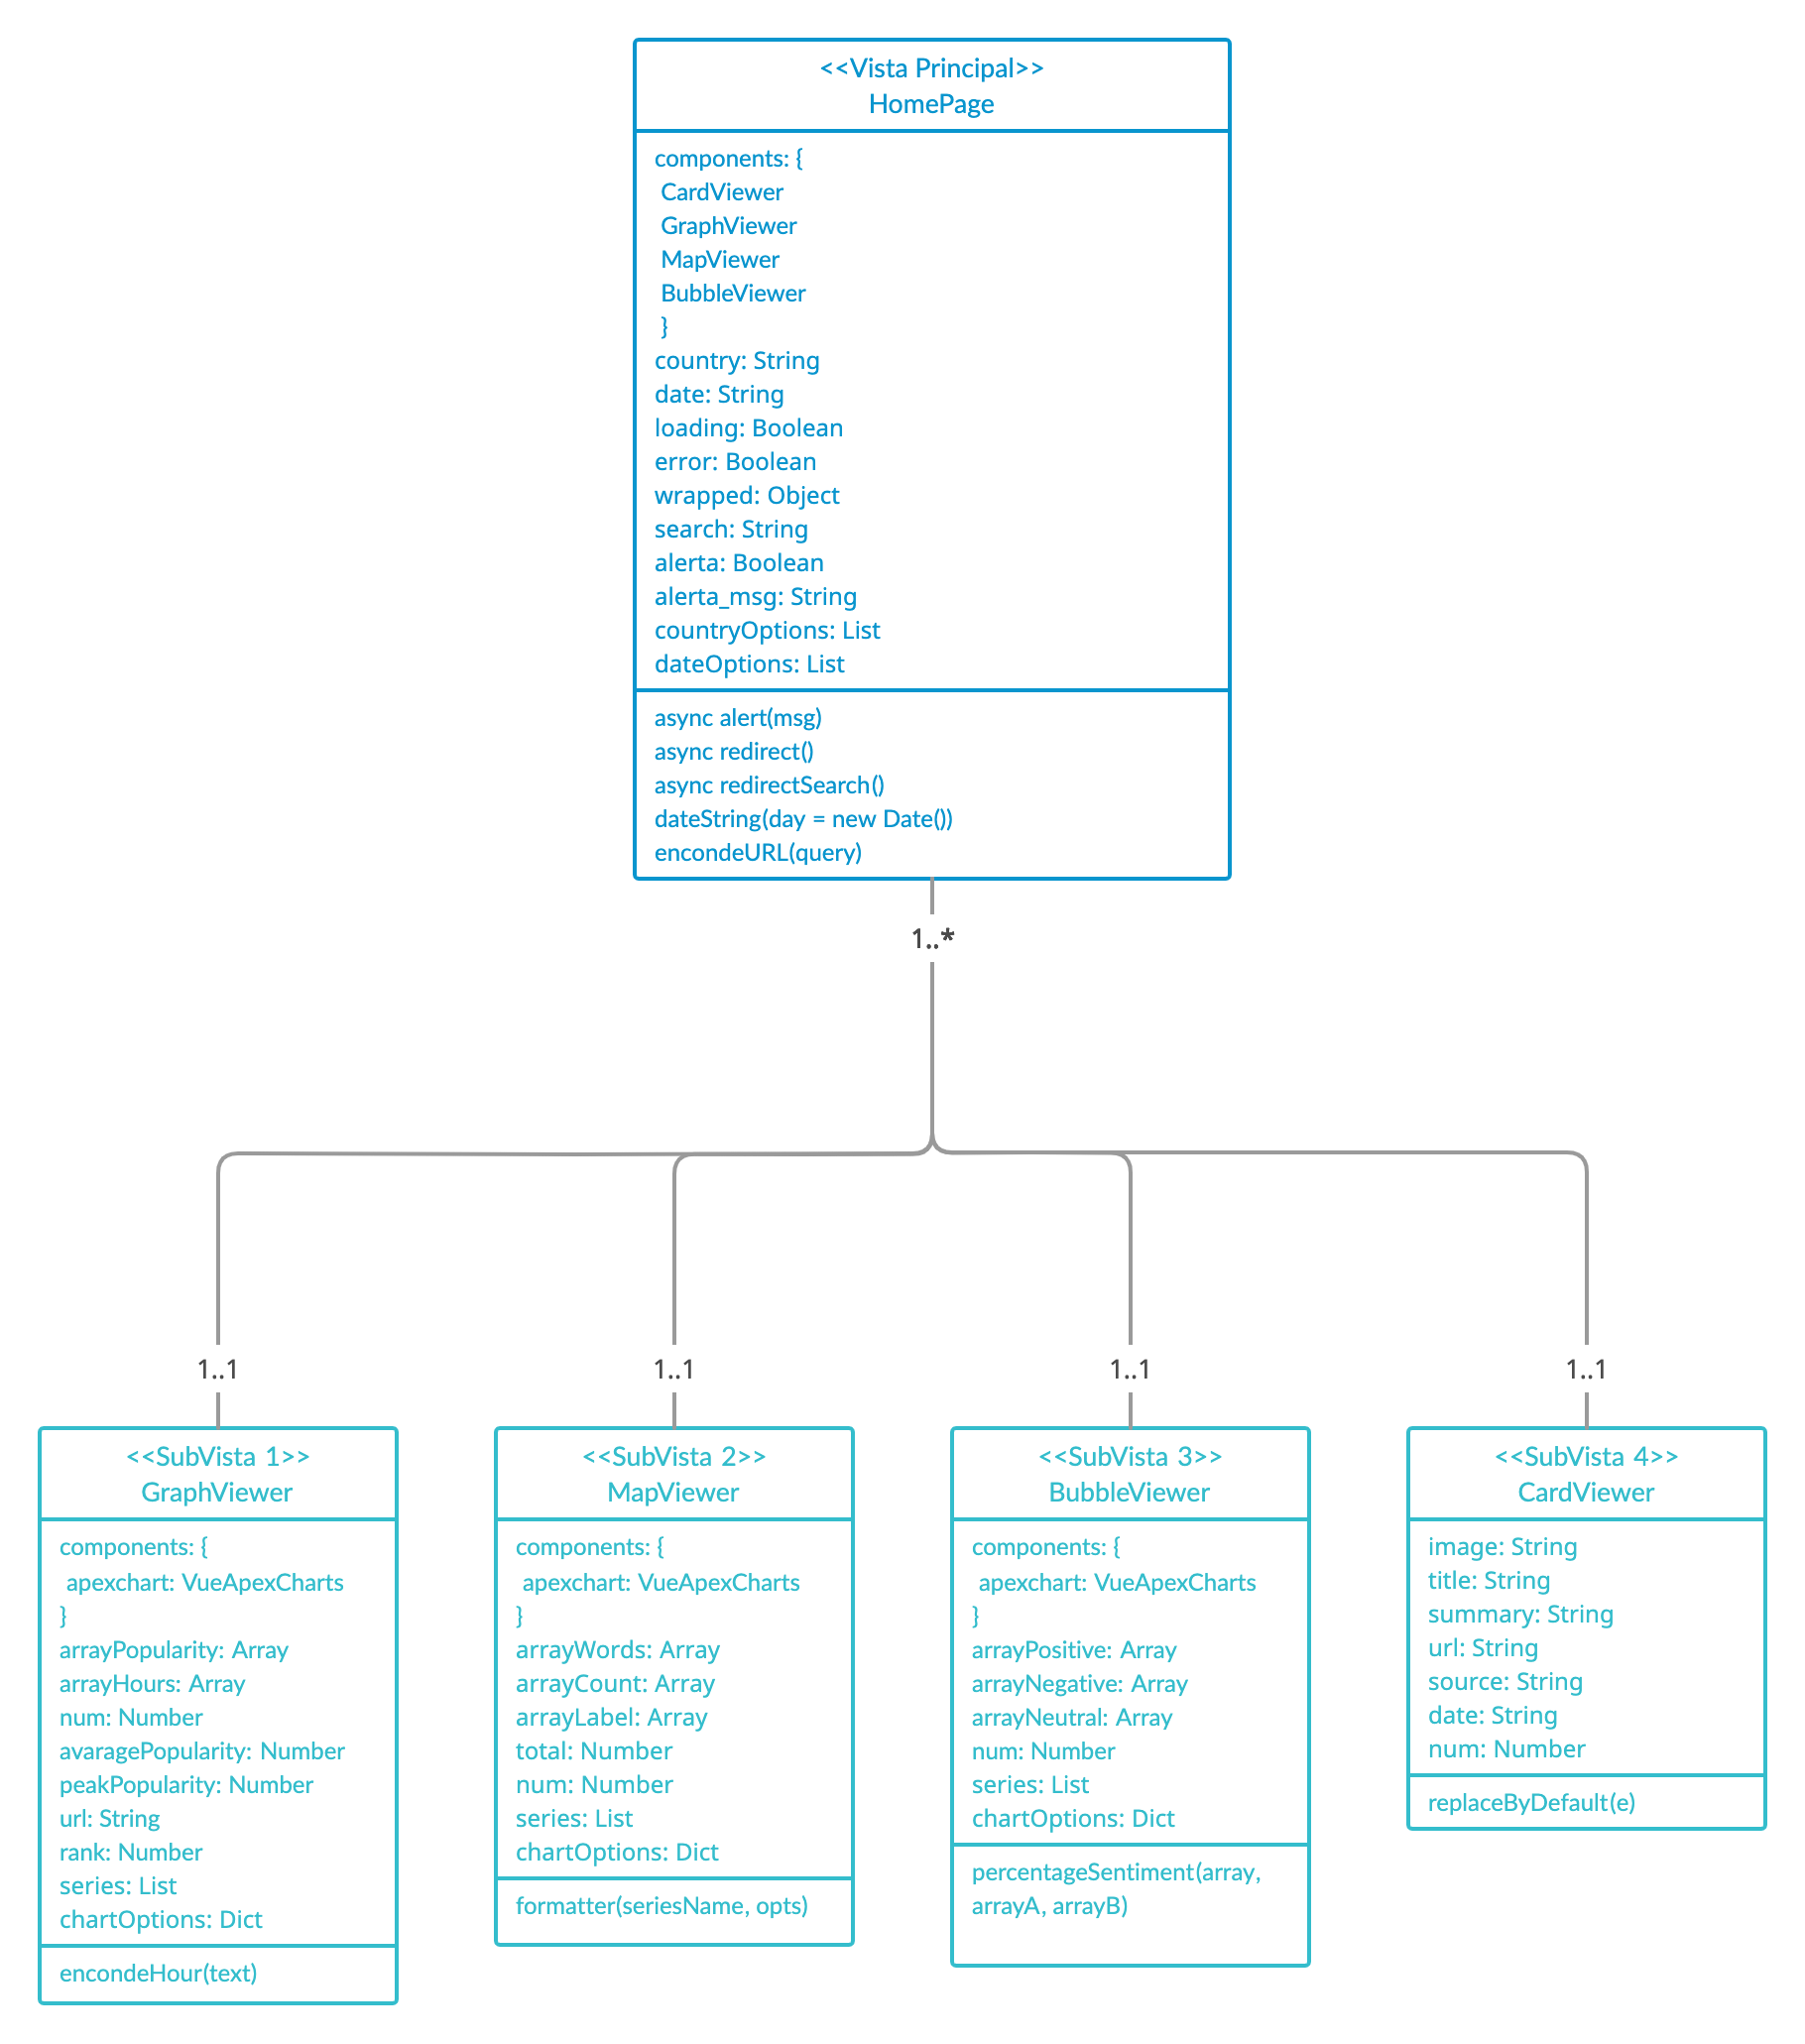
\includegraphics[width=1\textwidth]{gfx/Diagrama-de-Vistas.png}
    \caption[Diagrama de clase de las Vistas]{Diagrama de clase de las Vistas.}\label{gfx:Diagrama-de-Vistas}
\end{figure}

Cada subvista es llamada desde la vista principal, cada una con propiedades y funciones diferentes, ya que la representación de cada vista debe ser única y esencial.

\vspace{0.3cm}

La Vista principal representa la visualización de la historia de usuario que fue contemplada en el Sprint 2 (\ref{subs:sprint-2}) y esta relaciona con la entidad explicada en la sección \ref{subsub:ent-tendencia}. Esta vista es llamada \textit{HomePage} y está formada por \textit{components}, los cuales son las diferentes subvistas que se ha mencionado anteriormente. Los parámetros de las distintas rutas están referenciados por \textit{country}, \textit{date}, \textit{countryOptions} y \textit{dateOptions}, además las funciones de esta vista tienen el objetivo de construir los distintos formularios y los datos de la tendencia se cargarán en \textit{wrapped}.

\vspace{0.3cm}

También existen propiedades más complementarias como \textit{num} y \textit{rank}, para enumerar las tarjetas o cartas y el \textit{ranking} de la tendencia, respectivamente. Las funciones de alerta o los distintos atributos como \textit{loading}, existen para enriquecer las animaciones de la página y para mostrar el cuadro de dialogo que se ha mencionado anteriormente (\ref{gfx:boceto-error}). Finalmente, la función de \textit{encodeURL} codifica el nombre de la tendencia para redirigirlo a la plataforma Twitter mediante un enlace.

\subsection{Subvista Popularidad}
Esta subvista representa la visualización de las historias de usuario que fueron contempladas en el Sprint 6 (\ref{subs:sprint-6}). En ellas el usuario debe poder visualizar datos de interés sobre la popularidad y también un gráfica de área. La implementación de la gráfica se consigue mediante la librería ApexCharts.

\begin{figure}[H]
    \centering
    \myfloatalign
    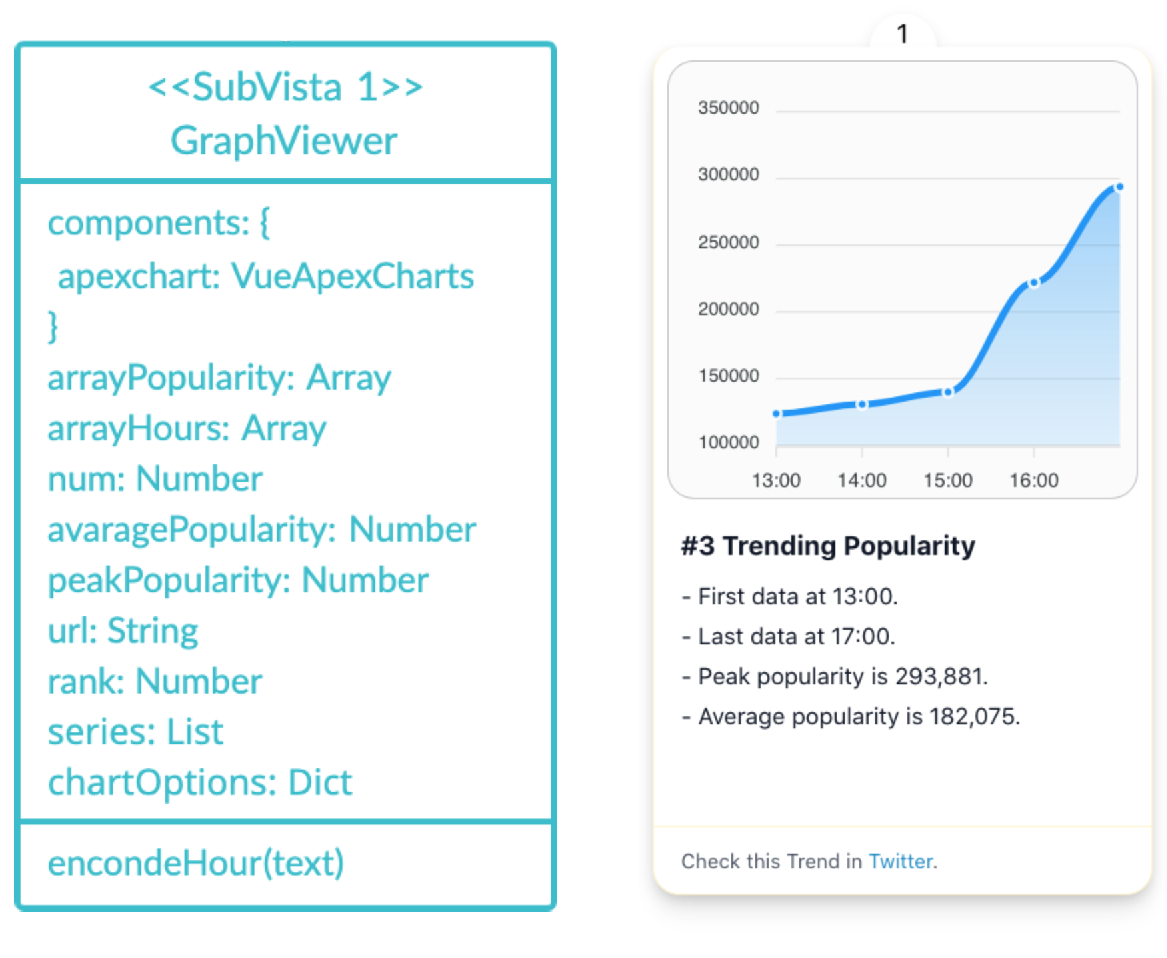
\includegraphics[width=0.9\textwidth]{gfx/subvista1.png}
    \caption[Estructura y Diseño de la primera subvista]{Estructura y Diseño de la primera subvista.}\label{gfx:subvista1}
\end{figure}

Los diferentes valores que posee esta subvista están relacionados con la entidad Popularidad (\ref{subsub:ent-popularidad}), a excepción de propiedades de la gráfica y atributos complementarios como \textit{url}, para redirigir a la plataforma de Twitter. La función debe transformar el texto en formato \textit{Date} de JavaScript.

\subsection{Subvista Palabras más Comunes y Keywords}
Esta subvista representa la visualización de las historias de usuario que fueron contempladas en el Sprint 7 (\ref{subs:sprint-7}). En ellas el usuario debe poder visualizar datos de interés sobre las palabras más comunes, las \textit{keywords} y un gráfico de radial de barras correspondiente. La implementación de la gráfica se consigue mediante la librería ApexCharts.

\begin{figure}[H]
    \centering
    \myfloatalign
    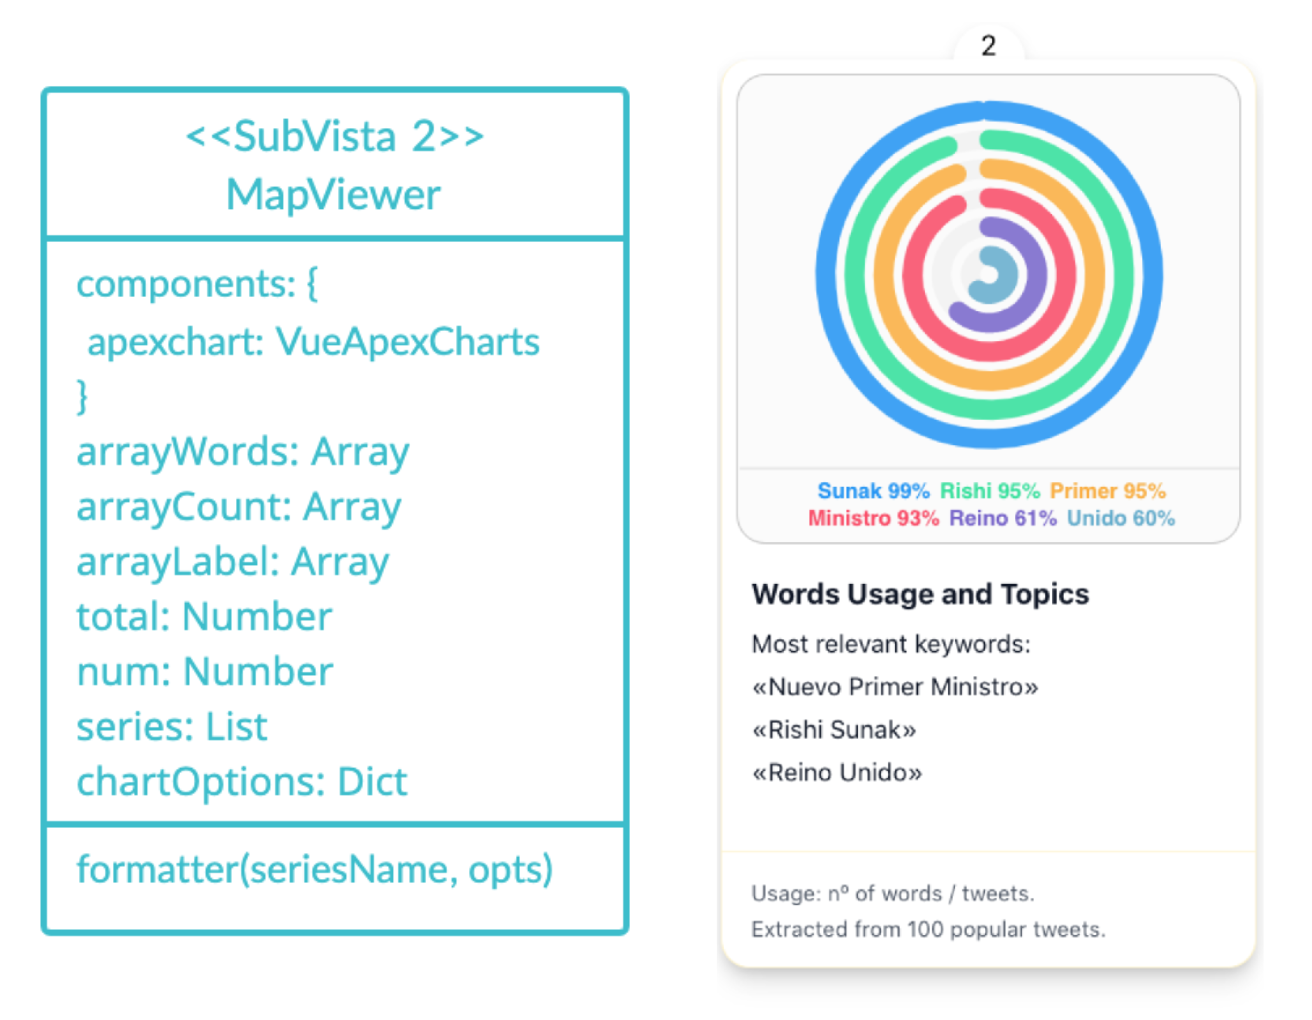
\includegraphics[width=0.9\textwidth]{gfx/subvista2.png}
    \caption[Estructura y Diseño de la segunda subvista]{Estructura y Diseño de la primera subvista.}\label{gfx:subvista2}
\end{figure}

Los diferentes valores que posee esta subvista están relacionados con la entidad explicada en la sección \ref{subsub:ent-keywords}. La función adapta el formato a los porcentajes.

\vspace{0.3cm}

Esta subvista tuvo un diseño inicial que fue descartado por problemas de diseño y también por posible confusión a la hora de interpretar el gráfico. El diseño tuvo problemas a la hora de encajar el gráfico en su encuadre y no quedaba muy claro el porcentaje de uso de las distintas palabras.

\begin{figure}[H]
    \centering
    \myfloatalign
    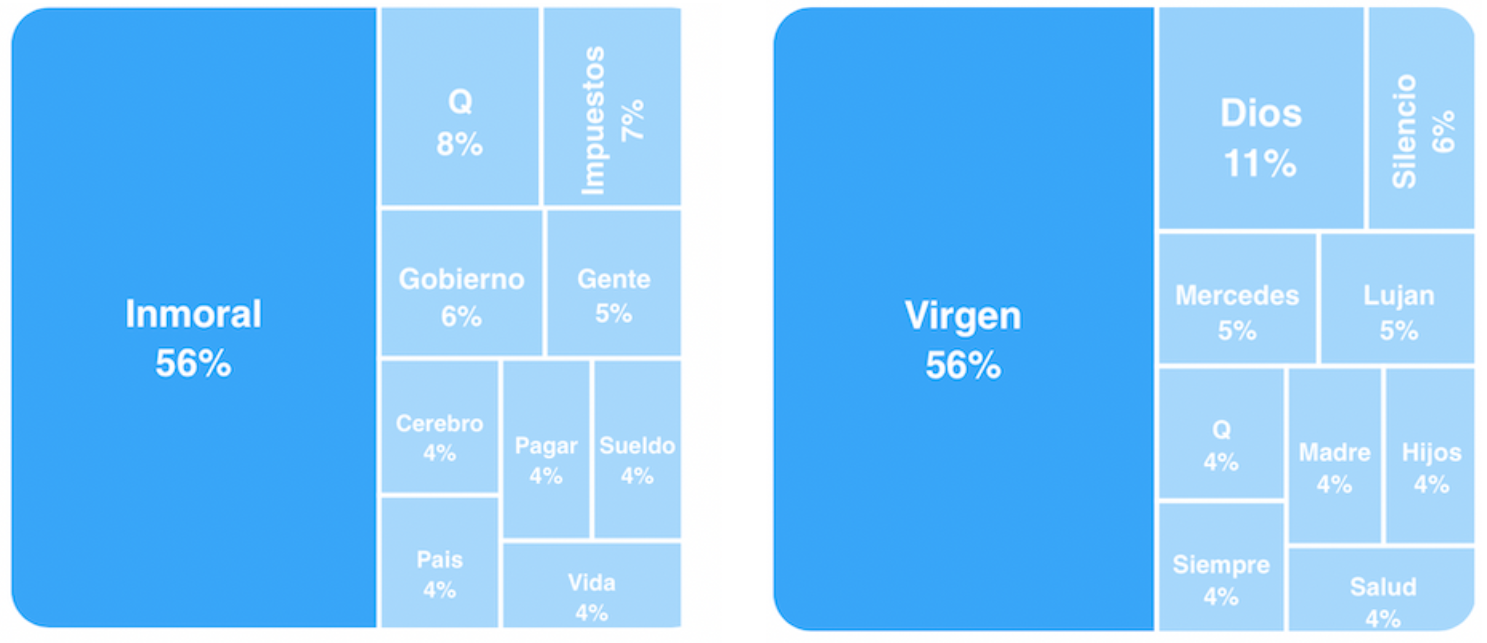
\includegraphics[width=0.8\textwidth]{gfx/subvista2-descartada.png}
    \caption[Diseño descartado de la segunda subvista]{Diseño descartado de la segunda subvista.}\label{gfx:subvista2-descartada}
\end{figure}

\subsection{Subvista Sentimiento General}
Esta subvista representa la visualización las historias de usuario que fueron contempladas en el Sprint 8 (\ref{subs:sprint-8}). En ellas el usuario debe poder visualizar datos de interés sobre el sentimiento general de los tweets o publicaciones y un gráfico de burbujas correspondiente. La implementación de la gráfica se consigue mediante la librería ApexCharts.

\begin{figure}[H]
    \centering
    \myfloatalign
    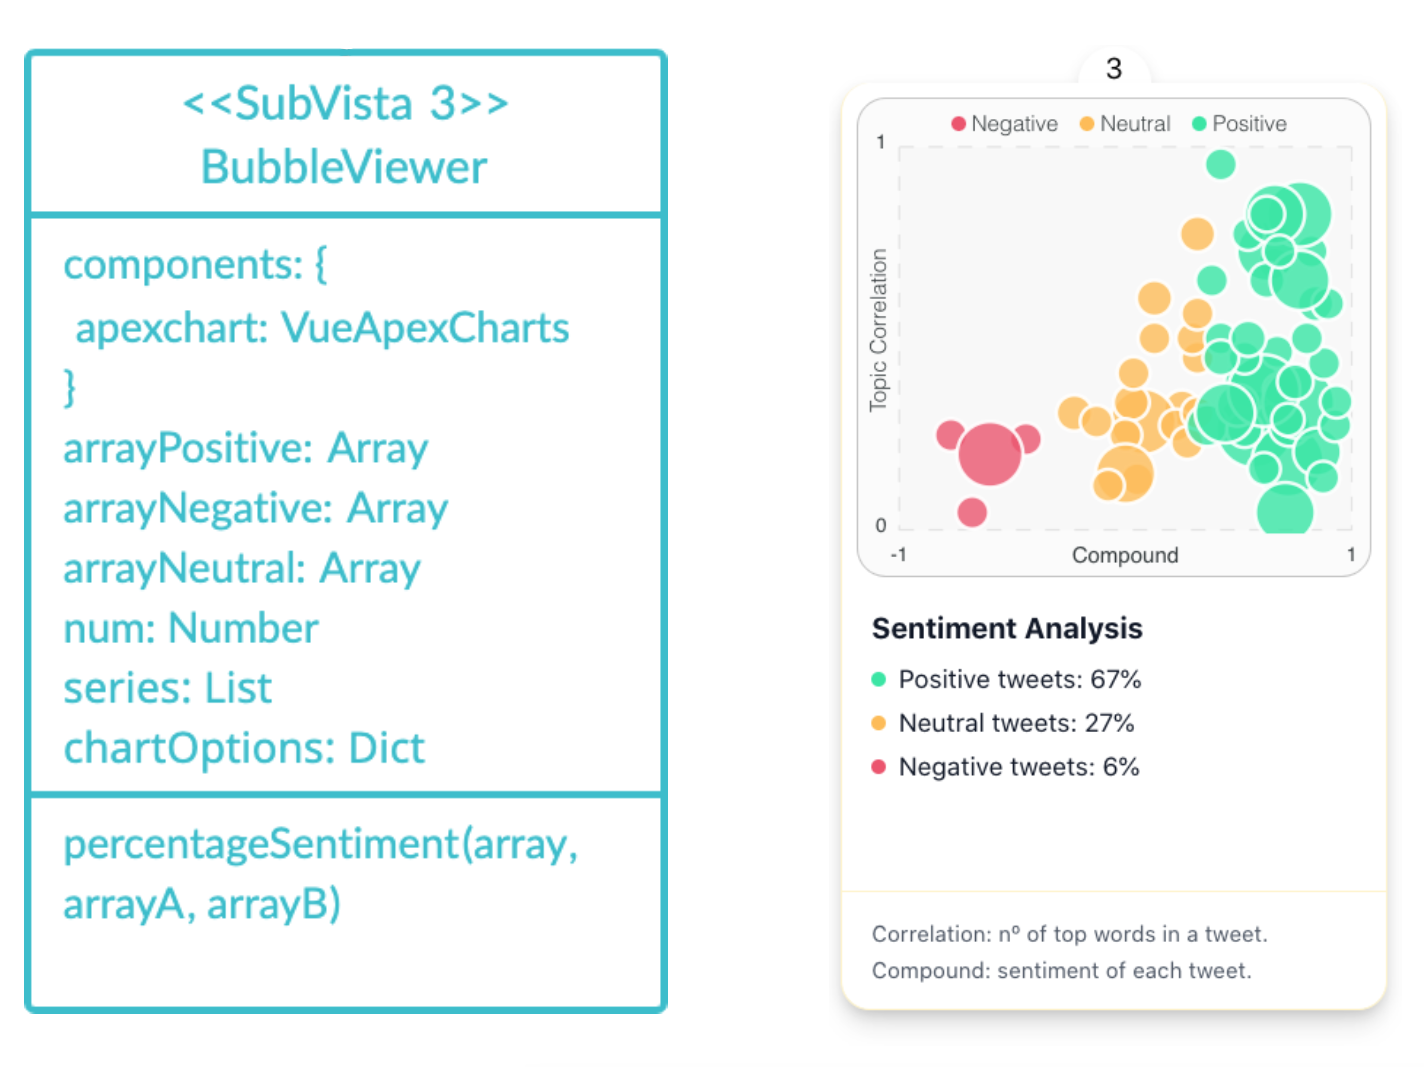
\includegraphics[width=0.9\textwidth]{gfx/subvista4.png}
    \caption[Estructura y Diseño de la tercera subvista]{Estructura y Diseño de la tercera subvista.}\label{gfx:subvista4}
\end{figure}

Los diferentes valores que posee esta subvista están relacionados con la entidad explicada en la sección \ref{subsub:ent-sentiment}. La función calcula el porcentaje dependiendo del radio de las burbujas.

\subsection{Subvista Noticas Relacionadas}
Esta subvista representa la visualización las historias de usuario que fueron contempladas en el Sprint 9 (\ref{subs:sprint-9}). En ellas el usuario debe poder visualizar datos de interés sobre las noticias o artículos relacionados sobre la tendencia.

\begin{figure}[H]
    \centering
    \myfloatalign
    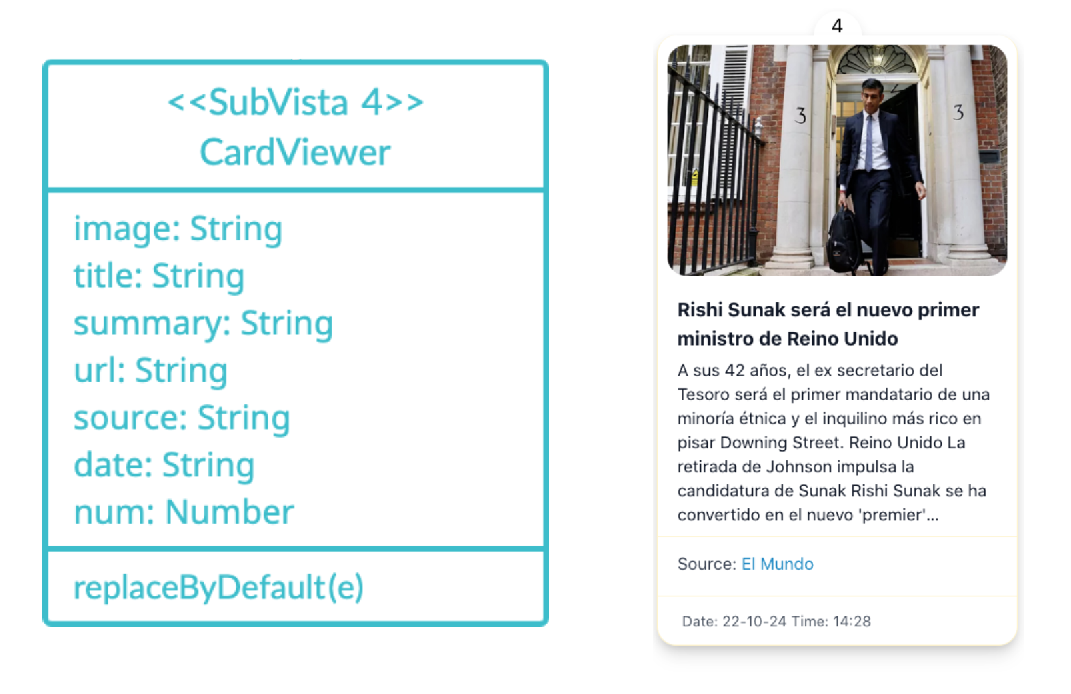
\includegraphics[width=0.9\textwidth]{gfx/subvista3.png}
    \caption[Estructura y Diseño de la última subvista]{Estructura y Diseño de la última subvista.}\label{gfx:subvista3}
\end{figure}

Los diferentes valores que posee esta subvista están relacionados con la entidad explicada en la sección \ref{subsub:ent-noticias}. La función devuelve una imagen por defecto si la carga de la imagen de la noticia falla.
	%\chapter{Terminología DevOps}\label{ch:devops}
%************************************************
Al haber consolidado la metodología de desarrollo SCRUM en los capítulos anteriores (\ref{sec:metodologia}), sabemos que dicha metodología pertenece a un ámbito de desarrollo iterativo e incremental, donde el proyecto se planifica en diversos bloques temporales. Debido a esto es muy frecuente que el equipo de desarrollo tenga numerosas entregas, ya que debe proporcionar una versión incrementada en cada iteración, esto también se suele denominar como despliegue.

\vspace{0.3cm}

Generalmente para proporcionar un despliegue el equipo de desarrollo se divide en dos ámbitos o departamentos. El primero tiene la función de desarrollo o la propia codificación de la aplicación, reconocido como «development» o «Dev» del inglés. El segundo se encarga de la parte operacional o el gestionado de versiones y la parte física del despliegue, reconocido también como «operations» o «Ops». \cite{redahat-devops}

\vspace{0.3cm}

El problema más usual es que ambos departamentos tienden a estar separados, por lo que el flujo de comunicación tiende a fallar y a tener retrasos a la hora de proporcionar el despliegue. Bajo esta premisa, surge una solución en 2009 denominada como \textit{DevOps}, la cual tiene como propósito unificar estos dos ámbitos \cite{redahat-devops}

\vspace{0.3cm}

\begin{figure}[H]
    \centering
    \myfloatalign
    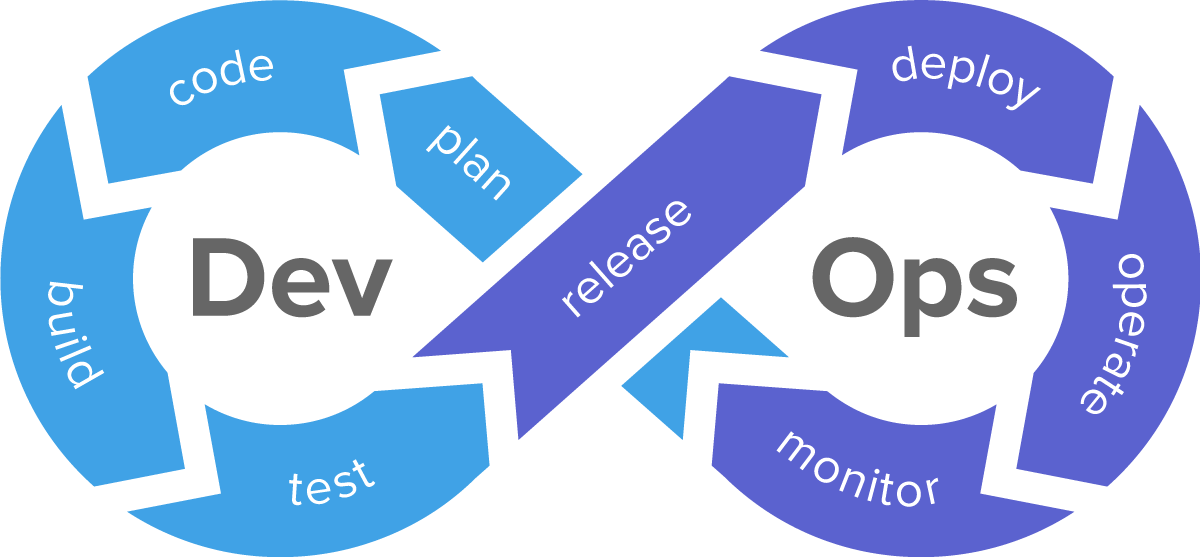
\includegraphics[width=0.7\textwidth]{gfx/devops-explicativo.png}
    \caption[Imagen explicativa del concepto DevOps]{Imagen explicativa del concepto DevOps \cite{azure-devops}.}\label{gfx:devops-explicativo}
\end{figure}

En resumen, \textit{DevOps} trata de romper estos silos organizativos establecidos y intenta centrarse en la mejora de calidad de la entrega al cliente. Para ello, \textit{DevOps} se apoya en tres principios o también llamadas «the three ways», las cuales se deben implementar de forma consecutiva. \cite{ilimit-devops}

\begin{enumerate}
    \item\textit{Mejora del flujo de entrega}: consiste en general valor al producto, mediante entregas del software de una forma temprana y periódica. Tratando de dividir los procesos en tareas más pequeñas o automatizando todas las tareas que sean posibles, con esto se consigue un aumento del flujo de trabajo global, ya que en este caso un proceso no ralentiza a otro. \\
    Un ejemplo de este principio puede ser la ejecución de tests u otras operaciones cada vez que haya cambios en el repositorio del código fuente.
    \item\textit{Buen uso de los ciclos de feedback}: consiste en el uso de la retroalimentación con el objetivo de optimizar los procesos, es decir, cada vez que se lleve a cabo una entrega conviene tener un \textit{feedback} rápido y constante. Con esto se que consigue que los ciclos de retroalimentación obtengan las información necesaria para que las correcciones se puedan aplicar de manera continua. \\
    Un ejemplo de ello puede ser la monitorización del sistema y la comunicación ante la detección de errores.
    \item\textit{Asentar el aprendizaje y la mejora continua}: se centra en aplicar todo lo anteriormente realizado y aprendido para implementar un sistema de mejora continua. De esta manera se consigue innovar el producto pero sin criminalizar los errores mediante el aprendizaje y las pruebas continuas. \\
    Un ejemplo puede llegar a ser usar programas extremos de pruebas o prestaciones.
\end{enumerate}

\subsection{Implementación Back-end}

Explicar Poetry, mypy, flake8 y pytest + esquema CI

\subsection{Implementación Front-end}
	%\part{Experiments and conclusions}\label{pt:results}
	%\chapter{Implementación}\label{ch:implmentacion}
%************************************************
Una vez habiendo establecido tanto la estructura como distintos conceptos de implementación, se puede empezar a incidir sobre diferentes implementaciones realizadas. El código fuente del proyecto, como he explicado en el capítulo anterior, está alojado en la plataforma de GitHub bajo el enlace de \url{https://github.com/nikitastetskiy/Wrapped}, el \textit{Back-end} en la plataforma Heroku bajo el enlace de \url{https://wrappedtrends.herokuapp.com} y el \textit{Front-end} en la plataforma Vercel bajo el enlace de \url{https://wrapped-trends.vercel.app}. Aún así, es conveniente analizar y explicar los diferentes códigos fuentes y algoritmos que se han implementado a lo largo del proyecto.

\section{Implementación Back-end}
La implementación de las capas pertenecientes a \textit{Back-end} se localizan en los directorios \textit{app} y \textit{backend}. El primero, guarda todas las entidades y \textit{scripts} necesarios para la obtención y gestión de datos de las tendencias. Mientras que el segundo guarda toda la estructura del servicio del servidor y el modelo perteneciente a la base de datos.

\subsection{Implementación Principal}
La primera implementación de código que se estudiará será la función principal encargada de gestionar las tendencias. Está denominada bajo el nombre de \textit{main\_operation}. Dicha función consigue las tendencias acordes al país y construye el diccionario apropiado, dependiendo de si existe dicho país en la base de datos o no. Si existe se tendrá que hacer una llamada de edición o PUT, en cambio si no existe se tendrá que crear y hacer una llamada POST. Además, se comprueba si existe un país con una antigüedad de más de 7 días para eliminarlo, con el objetivo de optimizar la base de datos.

\vspace{0.3cm}

En este primer caso, creo que es conveniente mostrar tanto el pseudocódigo como el código fuente de la función. En casos posteriores se alternará en base a la relevancia de la función, con el fin de optimizar la comprensión lectora.

\begin{algorithm}[H]\label{alg:offspring_fs}

    \Fn{Main}{

        \KwIn{country}
        trends $\longleftarrow$ getTrends(country)\;
        \If{\textit{trends}}{
            today = datetime.now(country)\;
            yesterday = today - 1\;
            oldCountry = requests.get(\textit{URI\_ENDPOINT})\;
            \If{oldCountry}{
                dict $\longleftarrow$ createDictCountry(country, trends, today, yesterday, oldCountry)\;
            } \Else{
                dict $\longleftarrow$ createDictCountry(country, trends, today, yesterday)\;
            }
            \If{\textit{dict}}{
                \If{oldCountry}{
                    requests.put(\textit{URI\_ENDPOINT}, dict.json())\;
                } \Else{
                    requests.post(\textit{URI\_ENDPOINT}, dict.json())\;
                    sevenDaysOldCountry = requests.get(\textit{URI\_ENDPOINT})\;
                    \If{\textit{sevenDaysOldCountry}}{
                        requests.delete(\textit{URI\_ENDPOINT})\;
                    }
                }
            }
        }
    }

    \caption{Operación Principal}

\end{algorithm}
\vspace{0.3cm}

La función tiene por \textit{input} \textit{country}, el cual es un diccionario con valores predefinidos que necesita cada país, es decir, valores como el nombre del país, el WOEID, el código del país, su lenguaje y su zona horaria. Otro valor predefinido es el \textit{endpoint} de mi servidor, para realizar llamadas HTTP.

\vspace{0.3cm}

\begin{lstlisting}[caption=Operación principal,          label={lst:listing-python},language=Python]
def main_operation(country):

    sorted_trends = get_trends_with_country(country['woeid'])
    if sorted_trends:

        DATE = datetime.now(
            timezone(country['timezone'])).strftime("%y-%m-%d")
        YESTERDAY = (datetime.now(timezone(country['timezone']))
                    - timedelta(days=2)).strftime("%Y-%m-%d")
        resp = requests.get(f"{TRENDING_WRAPPED_ENDPOINT}
                {country['name']}/{DATE}")

        # Checking if the object exists already
        if resp.status_code == 200:
            my_dict = create_dict_country(country,
                        sorted_trends, DATE, YESTERDAY,
                        json.loads(resp.content)["tendencias"])

        else:
            my_dict = create_dict_country(
                country, sorted_trends, DATE, YESTERDAY, False)

        if my_dict:
            my_dict_json = json.dumps(
                my_dict, default=lambda o: o.__dict__)
            my_headers = {
                'accept': 'application/json',
                'Content-Type': 'application/json'
            }
            # Checking if the object exists already
            if resp.status_code == 200:
                req = requests.put(
                    TRENDING_WRAPPED_ENDPOINT, data=my_dict_json,
                    headers=my_headers)
            else:
                req = requests.post(
                    TRENDING_WRAPPED_ENDPOINT, data=my_dict_json,
                    headers=my_headers)
                OLD_DATE = (datetime.now(timezone(
                            country['timezone'])) -
                            timedelta(days=7)).
                            strftime("%y-%m-%d")
                old_resp = requests.get(
                    f"{TRENDING_WRAPPED_ENDPOINT}
                    {country['name']}/{OLD_DATE}")
                # Checking for old objects
                if old_resp.status_code == 200:
                    old_resp = requests.delete(
                        f"{TRENDING_WRAPPED_ENDPOINT}
                        {country['name']}/{OLD_DATE}")
\end{lstlisting}

Para la creación de los diccionarios, el \textit{endpoint} y el acceso a la API de Twitter se han creado unas constantes globales. Se ha propuesto tres países relevantes como ejemplos. En cuanto al acceso a la API de Twitter se puede hacer de varias maneras, pero las funciones y los recursos de la API cambian dependiendo de la manera que se autentifique en la API. En este caso se ha hecho con V1, pero también se ha comentado la otra posibilidad.

\vspace{0.3cm}

\begin{lstlisting}[caption=Declaraciones de paises,          label={lst:listing-python},language=Python]
COUNTRIES = [
    {
        'name': 'Spain',
        'woeid': 23424950,
        'code': 'ES',
        'language': 'es',
        'timezone': 'Europe/Madrid'
    },
    {
        'name': 'United States',
        'woeid': 23424977,
        'code': 'US',
        'language': 'en',
        'timezone': 'US/Pacific'
    },
    {
        'name': 'Ukraine',
        'woeid': 23424976,
        'code': 'UA',
        'language': 'uk',
        'timezone': 'Europe/Kiev'
    }
]
\end{lstlisting}

\begin{lstlisting}[caption=Declaración de \textit{endpoint},          label={lst:listing-python},language=Python]
TRENDING_WRAPPED_ENDPOINT = "https://wrappedtrends.herokuapp.com/country/"
\end{lstlisting}

Cada proyecto iniciado en la API de Twitter proporciona claves de acceso o secretos únicos que no deben ser compartidos con nadie. Estos son utilizados para acceder y autenticarse en la API.

\vspace{0.3cm}

\begin{lstlisting}[caption=Autentificación de la API de Twitter,          label={lst:listing-python},language=Python]
# ENV VARIABLES OF TWITTER API
consumer_key = os.getenv('API_KEY')
consumer_secret = os.getenv('API_SECRET')
access_token = os.getenv('ACCESS_TOKEN')
access_token_secret = os.getenv('ACCESS_TOKEN_SECRET')

# TWITTER API
auth = tweepy.OAuthHandler(consumer_key, consumer_secret)
auth.set_access_token(access_token, access_token_secret)
api = tweepy.API(auth)

# client = tweepy.Client(bearer_token=BEARER_TOKEN)
\end{lstlisting}

La operación principal se tendrá que ejecutar para cada país, lo cual es bastante costoso, debido a que cada país o valor del diccionario tendrá que estar esperando hasta la finalización del valor que haya por delante. Debido a esto he implementado una función que se ejecute mediante el multiprocesamiento. La función recorre los diferentes países de manera asíncrona, bajo la premisa del número máximo de procesos que se pueden utilizar para ejecutar las llamadas dadas, en el caso dado es 200. Si no se proporciona, se crearán tantos procesos de trabajo como procesadores tenga la máquina.

\vspace{0.3cm}

\begin{lstlisting}[caption=Ejecución con multiprocesamiento,          label={lst:listing-python},language=Python]
def main():

    # Multiprocessing
    executor = concurrent.futures.ProcessPoolExecutor(200)
    futures = [executor.submit(main_operation, country) for country in COUNTRIES]
    concurrent.futures.wait(futures)

if __name__ == "__main__":

    main()
\end{lstlisting}


Por lo que algo que puede tardar minutos en ejecutarse de manera síncrona, lo hace en menos de un tercio de tiempo debido al multiprocesamiento, aunque la consumición de energía del procesador es mayor. En la siguiente imagen se pueden ver los resultados, la primera imagen será sin el multiprocesamiento y la segunda lo incluirá.

\begin{figure}[H]
    \centering
    \myfloatalign
    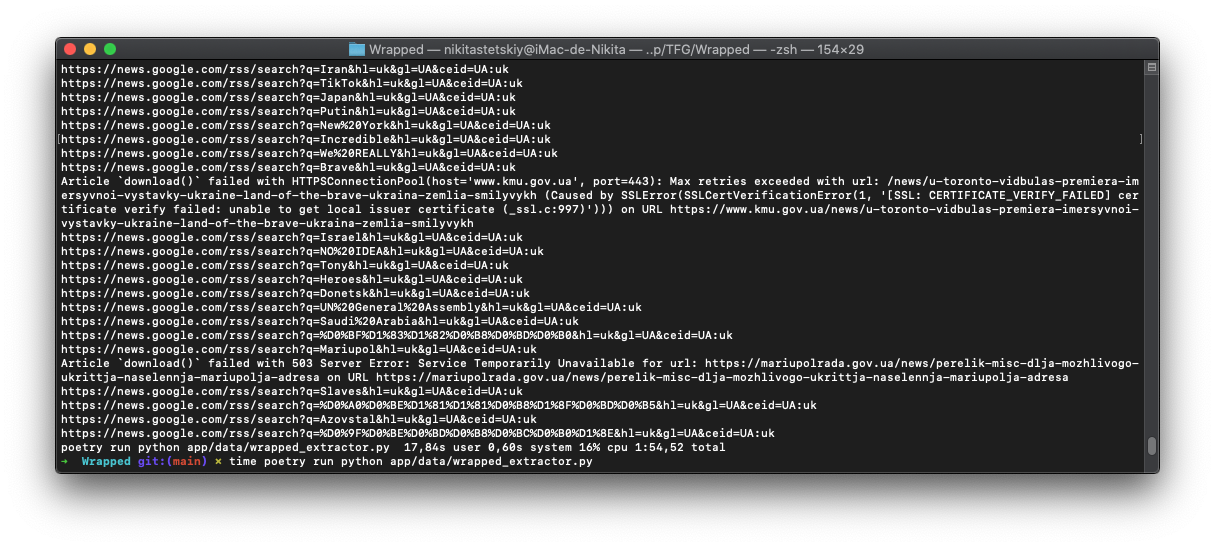
\includegraphics[width=1\textwidth]{gfx/comparacion-multiprocesamiento.png}
    \caption[Comparación de la ejecución sin multiprocesamiento]{Comparación de la ejecución sin multiprocesamiento.}\label{gfx:comparacion-multiprocesamiento}
\end{figure}

Aunque el mayor coste de la ejecución se basa en la descarga de diferentes artículos o noticias en base a la tendencia, esto es debido a que dependen del ancho de la red y su velocidad de descarga, la implementación de la función correspondiente se verá más adelante.

\begin{figure}[H]
    \centering
    \myfloatalign
    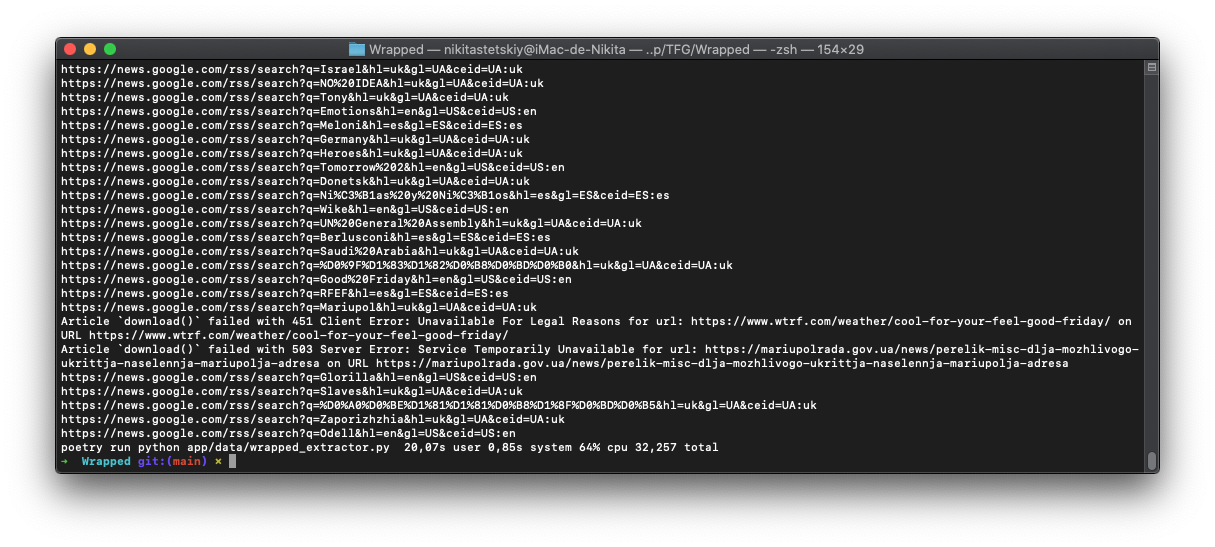
\includegraphics[width=1\textwidth]{gfx/comparacion-multiprocesamiento2.png}
    \caption[Comparación de la ejecución con multiprocesamiento]{Comparación de la ejecución con multiprocesamiento.}\label{gfx:comparacion-multiprocesamiento2}
\end{figure}

\subsection{Implementación de la Generación del Diccionario}
La generación del diccionario a simple vista puede parecer sencilla, ya que solo tenemos que descargar los nombres de las tendencias y convertirlos en distintos objetos para que la base de datos pueda interpretarlos. Aunque esto se puede complicar debido a varios factores.

\vspace{0.3cm}

Primero, si se tiene un objeto ya creado en la base de datos, pues se tendrá que descargarlo y compararlo con el nuevo. Esto es debido a que las tendencias cambian cada hora y se debe tener en cuenta las tendencias viejas y sus distintos atributos. Por lo que se hará una unión entre las tendencias nuevas y las viejas, y posteriormente una diferencia simétrica entre las tendencias restantes con el objetivo de actualizar los atributos de tendencias viejas o incorporar tendencias completamente nuevas. Luego, se tiene que realizar distintas llamadas con distintos parámetros a la API de Twitter, con la intención de crear diferentes objetos funcionales y agregarlos al diccionario (objetos como la popularidad, los sentimientos o artículos).

\vspace{0.3cm}

Al descargar tendencias nuevas y compararlas con las viejas, se hará unión si hay tendencias bajo el mismo nombre. Esto es debido a que es necesario actualizar atributos como la popularidad, pero a la vez mantener el historial del volumen de publicaciones. Luego, la diferencia simétrica se refiere a las tendencias que no aparecen en la unión, ellas también estarán en cuenta a la hora de ordenar la lista de tendencias bajo el valor de la popularidad.

\begin{algorithm}[H]

    \Fn{createDictCountry}{

        \KwIn{country, sortedTrends, date, yesterday, oldTrends}
        \KwOut{dictCountry}
        sortedParsed $\longleftarrow$ $\emptyset$\;
        hour = datetime.now(country)\;
        cont = 0\;
        \If{\textit{oldTrends}}{
            sortedParsed $\longleftarrow$ parseTrend(sortedTrends) $\cup$ oldTrends\;
            sortedParsed $\longleftarrow$ sortedParsed $\triangle$ oldTrends\;
        } \Else{
            sortedParsed = parseTrend(sortedTrends)
        }
        \While{cont $\neq$ 10}{
            tweets $\longleftarrow$ api.searchTweets($sortedParsed_{cont}$)\;
            keywords $\longleftarrow$ searchKeywords(tweets)\;
            sentiments $\longleftarrow$ searchSentiments(tweets)\;
            articles $\longleftarrow$ searchArticles(tweets)\;
            cont++\;
        }
        dictCountry = dictCountry(keywords, sentiments, articles)\;
        \KwRet dictCountry\;
    }

    \caption{Creación del Diccionario Country}

\end{algorithm}

\vspace{0.3cm}

Habiendo entendido el pseudocódigo podemos comprender de una manera más sencilla el código fuente. Primero se comprueba si existen tendencias viejas, después se procedería a asignar una estructura constituyente a dichas tendencias mediante la unión y la diferencia simétrica. Además, sólo se procede al final con 20 tendencias y se calcula su popularidad, esto es debido a la optimización de la base de datos y su gestión. Posteriormente se calculan los demás valores (keywords, sentimientos y artículos) sobre la mitad de las tendencias clasificadas, es decir, un top 10. Las otras diez tendencias, que no llegaron a clasificarse, sirven como referencia posteriormente a la hora de pintar el gráfico de la popularidad, ya que esa información sigue siendo relevante, como historial, si la tendencia llega a ser mostrada.

\vspace{0.3cm}

\begin{lstlisting}[caption=Creación de la estructura de tendencias,          label={lst:listing-python},language=Python]
if old_trends:
    for item in sorted_trends:
        t = parse_trend(item['name'], item['tweet_volume'],
        hour, None)
        for k, old_item in enumerate(old_trends):
            if old_item["name"] == item["name"]:
                t.popularity.refresh(old_item["popularity"]
                        ["volume"],old_item["popularity"]
                        ["hour_popularity"])
                old_trends.pop(k)
                break
        sorted_parsed.append(t)
    for i in old_trends:
        sorted_parsed.append(Trend(**i))

# When there aren't any new trends on the platfrom yet
else:
    for item in sorted_trends:
        t = parse_trend(item['name'], item['tweet_volume'],
            hour, None)
        sorted_parsed.append(t)

sorted_parsed = comparing_names(sorted_parsed)
sorted_parsed = sorted(sorted_parsed, key=lambda trend:
    trend.popularity.peak_popularity, reverse=True)[:20]
\end{lstlisting}

Una vez teniendo la estructura y los objetos de las tendencias, podemos proceder a calcular los demás valores, donde necesitaremos descargar como máximo cien publicaciones o tweets relacionadas con la tendencia. Primero se hace una llamada a la API con determinado valor hacia el ámbito popular. Se filtran las publicaciones repetidas y se intenta que sean publicaciones populares, si no se consiguen se opta por publicaciones menos famosas. Además, sólo se procede a asignar los valores una vez habiendo calculado todos ellos, para que solo existan objetos completos a la hora de visualizarlos.

\vspace{0.3cm}

\begin{lstlisting}[caption=Creación de la estructura constituyente,          label={lst:listing-python},language=Python]
wts = 0
while wts < 10 and cont < len(sorted_parsed):
    name = sorted_parsed[cont].name
    tweets = api.search_tweets(q=f'{name} -filter:retweets
            min_faves:20 since:{yesterday}', lang=country
            ["language"], count=100, result_type="mixed",
            tweet_mode="extended")
    if (len(tweets)) < 50:
        tweets = api.search_tweets(q=f'{name} -filter:retweets
            since:{yesterday}', lang=country["language"],
            count=100, result_type="mixed",
            tweet_mode="extended")
    t = get_tweets(tweets, country["language"])
    if t:
        name = more_specific_name(t.words, name)
        w = get_wrappeds(name, country["code"],
            country["language"])
        if w:
            s = get_sentiments(tweets, country["language"],
                t.label)
            if s:
                sorted_parsed[cont].wrappeds = w
                sorted_parsed[cont].keywords = t
                sorted_parsed[cont].sentiments = s
                wts += 1
    cont += 1

dict_country = {
    'pais': country["name"],
    'dia': date,
    'tendencias': sorted_parsed
}

return dict_country
\end{lstlisting}

La búsqueda de un tópico funcionaría de la misma manera, pero solo consiguiendo un solo objeto completo. También se limita el cálculo de la popularidad, ya que esa información proviene de las tendencias de la API de Twitter. Por lo que las únicas diferencias a la hora de implementarlo serían las funciones de estructuración.

\vspace{0.3cm}

\begin{lstlisting}[caption=Estructuración de la tendencia,          label={lst:listing-python},language=Python]
# PARSING OBJECT TREND
def parse_trend(name, vol, time, array):

    popularity = parse_popularity(vol, time)

    values = {
        'name': name,
        'popularity': popularity,
        'wrappeds': array
    }

    return Trend(**values)

# PARSING OBJECT SINGLE TREND
def parse_single_trend(name, array):

    values = {
        'name': name,
        'popularity': None,
        'wrappeds': array
    }

    return Trend(**values)
\end{lstlisting}

A la hora de descargar las tendencias de Twitter, se tiene que comparar los nombres de distintas tendencias tal como se ha comentado en las tareas de la Historia de Usuario del Sprint 2 (\ref{subs:sprint-2}). Para ello se comprueban si hay parecidos en los nombres, sin contemplar las mayúsculas, minúsculas y tildes. Por lo que para ello se han creado dos funciones, una normaliza una oración (quitando tildes, mayúsculas y caracteres de puntuación) y la otra recorre las distintas tendencias en busca de parecidos.

\vspace{0.3cm}

\begin{lstlisting}[caption=Comprobación de los nombres de tendencia,          label={lst:listing-python},language=Python]
def normalize_str(c):
    s = string.punctuation + " "
    return c.translate(str.maketrans("áéíóú","aeiou", s)).lower()

def comparing_names(s):
    i = 0
    while i < (len(s)-1):
        j = i+1
        while j < (len(s)):
            if normalize_str(s[j].name) in normalize_str(s[i].
            name) or normalize_str(s[i].name) in 
            normalize_str(s[j].name):
                if len((s[i].name).split()) > len((s[j].name).
                split()):
                    s.pop(j)
                    j -= 1
                elif len((s[i].name).split()) < 
                len((s[j].name).split()):
                    s.pop(i)
                    i -= 1
                    break
                else:
                    if s[j].popularity.peak_popularity >= s[i].
                    popularity.peak_popularity:
                        s.pop(i)
                        i -= 1
                        break
                    else:
                        s.pop(j)
                        j -= 1
            j += 1
        i += 1

    return s
\end{lstlisting}

\subsection{Implementación de la Popularidad}
La entidad Popularidad está compuesta por distintos valores comentados en la sección \ref{subsub:ent-popularidad}. Dentro de la entidad Popularidad está la función que actualiza los valores y se calculan con una librería popular orientada hacia campo matemático llamada \textit{numpy}.

\vspace{0.3cm}

\begin{lstlisting}[caption=Estructuración de la popularidad,          label={lst:listing-python},language=Python]
# PARSING OBJECT POPULARITY
def parse_popularity(vol, time):

    values = {
        'volume': [vol],
        'hour_popularity': [time],
        'avarage_popularity': vol,
        'peak_popularity': vol,
    }

    return Popularity(**values)
\end{lstlisting}

\begin{lstlisting}[caption=Actualización de la popularidad,          label={lst:listing-python},language=Python]
def refresh(self, vol, hour):
    self.volume = vol + self.volume
    self.hour_popularity = hour + self.hour_popularity
    self.avarage_popularity = int(np.average(self.volume))
    self.peak_popularity = int(np.max(self.volume))
\end{lstlisting}

\subsection{Implementación de las \textit{Keywords}}
La entidad \textit{Keyword} está compuesta por distintos valores comentados en la sección \ref{subsub:ent-keywords}.

\vspace{0.3cm}

\begin{lstlisting}[caption=Estructuración de las keywords,          label={lst:listing-python},language=Python]
# PARSING OBJECT KEYWORD
def parse_keyword(k):

    values = {
        'total': k['total'],
        'count': k['count'],
        'label': k['label'],
        'words': k['words'],
    }

    return Keyword(**values)

def get_tweets(tweets, lng):

    t = fetch_tweets(tweets, lng)
    if t:
        t = parse_keyword(t)
        return t
    else:
        return False
\end{lstlisting}

A la hora de extraer las \textit{keywords}, de los distintos tweets o publicaciones descargados de la API de Twitter, se deben limpiar tal y como se comentó en el Sprint 7 (\ref{subs:sprint-7}). Para ello se implementaron varias versiones para comprobar la eficiencia de cada una de ellas. Primero un sistema regex, luego el sistema regex de numpy y por último funciones de sintaxis de Python. Finalmente, las más eficientes fueron las expresiones regex o expresiones regulares. La siguiente captura de código fue para comprobar los distintos tiempos de ejecución, muchos de ellos fueron similares, pero las expresiones regex siempre tuvieron resultados ventajosos y que a la larga resultarían mucho más beneficiosos en tiempos de cómputo.

\vspace{0.3cm}

\begin{lstlisting}[caption=Limpieza de las publicaciones,          label={lst:listing-python},language=Python]
def clean1(text):
    text = text.lower()
    # Removes all mentions (@username) from the tweet since it is of no use to us
    text = re.sub(r'@[\w]*', '', text)
    # Removes any link in the text
    text = re. sub(r'http://\S+ https://S+', '', text)
    # Only considers the part of the string with char between a to z or digits and whitespace characters
    # Basically removes punctuation
    text = re.sub(r'[^\w\s]', '', text)
    
def remove_pattern(input_txt, pattern):
    r = re.findall(pattern, input_txt)
    for i in r:
        input_txt = re.subli, '', input_txt)
    return input_txt
    
def clean2(tweets):
    # remove twitter handles (xxx)
    tweets = np.vectorize(remove_pattern)(tweets, "@[\w] *")
    # remove URL links (httpxxx)
    tweets = np.vectorize(remove pattern)(tweets,
            "https?://(A-Za-z0-9./1*")
    # remove special characters, numbers, punctuations
    tweets = np.core.defchararray.replace(tweets,
            "[^a-zA-Z]", " ")
    return tweets
    
def clean3(tweet):
    # Removing twitter handles which start with @ or #  ' or http
    tweet = ''.join(word for word in tweet.split(' ') if not
            (word.startswith('#') or word.startswith('@') or
            word.startswith("'") or word.startswith('http'))
    tweet = tweet.translate(str.maketrans('áéíóú',
            'aeiou')).lower()
    return(tweet)
\end{lstlisting}

Al final se estableció las expresiones regex como función definitiva y se procedió a implementar la manera de limpiar las palabras vacías o \textit{stop\_words}. La eliminación de palabras vacías solamente se utiliza en el recuento de frecuencia de palabras.

\vspace{0.3cm}

\begin{lstlisting}[caption=Limpieza de las publicaciones implementada,          label={lst:listing-python},language=Python]
def load_stop_words(file): 
    """
    Utility function to load stop words from a file and return as a list of words
    """
    with open(file, 'r+') as f:
        stop_words = f.read().splitlines()
    return set(stop_words)

def simple_clean(text):
    text = text.translate(str.maketrans('áéíóú', 'aeiou')).lower()
    # Removes all mentions (@username) or hashtags from the tweet since it is of no use to us
    text = re.sub(r'@[\w]*|#[\w]*', '', text)
    # Removes any link in the text
    text = re.sub(r'http://\S+|https://\S+', '', text)
    # Removes any \n
    text = re.sub(r'\n', ' ', text)

    return text

def clean(text, lng):
    # Basically removes punctuation
    text = re.sub(r'[^\w\s]', '', text)
    # Removes stop words that have no use in sentiment analysis
    stopwords = load_stop_words(f"app/data/ml_stopwords/my-{lng}-stopwords.txt")
    text = " ".join([word for word in text.split() if word
            not in stopwords])

    return text
\end{lstlisting}

Las dos funciones de limpieza existen porque una se usa en el recuento de palabras y la otra en la propia extracción de \textit{keywords}, la extracción de \textit{keywords} o palabras clave se hará mediante un algoritmo de extracción. Para ello se han estudiado varios algoritmos, entre ellos \ac{YAKE}, \ac{RAKE} y las herramientas de \ac{NLTK}. El más eficiente y eficaz resultó ser \ac{YAKE}, primero quedó descartado \ac{NLTK} ya que debía ser descargado a la hora de ejecución, por lo que tardaba más. \ac{RAKE} en cambio, solía tardar casi el mismo tiempo en ejecutarse, aunque su principal problema es que no reconocía distintas entidades como nombres o acrónimos («CEO» ó «Google»), algo fundamental en los tweets, por lo que muchas \textit{keywords} extraídas no contenían mucha relevancia.

\vspace{0.3cm}

Otra de las ventajas de \ac{YAKE} es que se puede configurar el idioma, la limitación de duplicación de claves o la cantidad de palabras en una \textit{keyword}. El sistema de \ac{YAKE} se rige por seis componentes: preprocesamiento de texto, extracción de características, puntaje de términos individuales, generación de listas de palabras clave candidatas, reduplicación de datos y clasificación. A continuación se explicarán las distintas etapas del algoritmo, pero se recomienda la lectura del libro \textit{YAKE! Collection-Independent Automatic Keyword Extractor} para su completo entendimiento. \cite{yake-libro}

\vspace{0.3cm}

Primero, se aplica una etapa de preprocesamiento, la cual divide el texto en términos individuales cada vez que se encuentra un espacio vacío o un carácter especial (por ejemplo, saltos de línea, corchetes, coma, punto, etc.). En segundo lugar, se diseñan un conjunto de cinco rasgos para capturar las características de cada término individual. Estos son: \textit{Casing}, \textit{Word Positional}, \textit{Word Frequency}, \textit{Word Relatedness to Context} y \textit{Word DifSentence}.

\vspace{0.3cm}

El primero, refleja el aspecto de \textit{casing} de una palabra (capitalización en castellano). \textit{Word Positional} valora más aquellas palabras que aparecen al principio de un documento basándose en la suposición de que las palabras clave relevantes a menudo tienden a concentrarse más al principio de un documento. \textit{Word Frequency} indica la frecuencia de la palabra, puntuando más aquellas palabras que aparecen con mayor frecuencia. La cuarta función, \textit{Word Relatedness to Context}, calcula el número de términos diferentes que aparecen delante o atrás de la palabra candidata. Cuanto mayor sea el número de términos diferentes que coexisten con la palabra candidata (en ambos lados), es probable que la palabra candidata carezca más de sentido. Finalmente, \textit{Word DifSentence} cuantifica con qué frecuencia aparece una palabra candidata dentro de diferentes oraciones.

\vspace{0.3cm}

En el tercer paso, se combina heurísticamente todas estas características en una sola medida, de modo que a cada término se le asigna una puntuación S(w). Este peso dará lugar al proceso de generación de palabras clave del cuarto paso. Se considera una ventana deslizante de 3 gramos, generando así una secuencia contigua de palabras clave candidatas de 1, 2 y 3-gramos. A cada palabra clave candidata se le asignará una S(kw) final, de modo que cuanto menor sea la puntuación, más significativa será la palabra clave. De esta manera se formaliza la siguiente ecuación.

\begin{equation}
S(kw)=\frac{\prod_{_{w \in kw}}^{}S(w)}{TF(kw)*(1+\sum_{w \in kw}^{}S(w))}
\end{equation}

S(kw) es la puntuación de una palabra clave candidata, determinada multiplicando (en el numerador) la puntuación S(w) del primer término de la palabra clave candidata por las puntuaciones posteriores de los términos restantes. Esto se divide por la suma de las puntuaciones de S(w) para promediar la longitud de la palabra clave, de modo que los n-gramos más largos no se beneficien solo porque tienen una \textit{n} más alta. El resultado se divide aún más por TF(kw) (frecuencia del término de la palabra clave) para penalizar a los candidatos menos frecuentes. En el quinto paso, se eliminan candidatos similares provenientes de los pasos anteriores. Para ello se usa la \textit{distancia de Levenshtein} \cite{levenshtein1966binary}. Finalmente, el sistema generará una lista de palabras clave relevantes, formada por 1, 2, 3-gramos, de modo que cuanto menor sea la puntuación de S(kw), más importante será la palabra clave.

\vspace{0.3cm}

En el siguiente código se puede ver la implementación de la librería \ac{YAKE} y el recuento de palabras relevantes. Además las \textit{keywords} extraídas pasan por un filtro, comprobando las repeticiones y un umbral mínimo de S(kw). Cabe señalar que estas funciones poseen un manejo de errores que no se muestran para facilitar la lectura.

\vspace{0.3cm}

\begin{lstlisting}[caption=Extracción de recuento de palabras y \textit{keywords},          label={lst:listing-python},language=Python]
texto = ''
for tweet in query: # Cleans the tweet
    clean_txt = simple_clean(tweet.full_text)
    texto += clean_txt + ' '
keywords = (clean(texto, lng).split())
counter = Counter(keywords)
data: dict[str, Any] = {
    'total': len(query),
    'count': [],
    'label': [],
    'words': []
}
for x, y in counter.most_common(6): # Words Counter
    data['label'].append(x)
    data['count'].append(round((y/len(query)) * 100))
    
# YAKE Extraction
stopwords = load_stop_words(f"app/data/ml_stopwords/
            my-{lng}-stopwords.txt")
custom_kw_extractor = yake.KeywordExtractor(
    lan=lng, n=3, dedupLim=0.6, dedupFunc="seqm",
    top=15, stopwords=stopwords, windowsSize=1)
yake_keywords = custom_kw_extractor.extract_keywords(texto)
yake_keywords = comparing_names(yake_keywords)
for k in yake_keywords:
    data['words'].append(k)

return data
\end{lstlisting}

El algoritmo \ac{YAKE} se rige por parámetros como la función de duplicación o la cantidad de \textit{keywords} extraídas. Estos parámetros fueron seleccionados cuidadosamente, para que finalmente solo se muestren tres \textit{keywords}. En un principio se extraen quince, pero al pasarlos por el filtro se quedarían en tres como máximo. En cambio, el contador de palabras es seis como máximo. El filtro intenta guardar las palabras claves más relevantes, por lo que elimina las repetidas.

\vspace{0.3cm}

\begin{algorithm}[H]

    \Fn{comparingNames}{
        \KwIn{setTuple}
        \KwOut{left(setOut, 3)}
        setOut $\longleftarrow$ $\emptyset$\;
        \tcp{Filtrado de palabras repetidas en una \textit{keyword}}
        
        \For{$s$ $\in$ $setTuple$}{
            words = s[0].split()\;
            $setOut$ $\longleftarrow$ set(words).toString()\;
            \tcp{Umbral de \textit{S(kw)}}
            \If{s[1] > 0.05}{
                \textbf{break}\;
            }
        }
        \tcp{Filtrado \textit{keywords} similares o repetidas}
        
        i = 0\;
        \While{i < $setOut$.size()-1 \textbf{and} $setOut$.size() > 3}{
            j = i+1\;
            \While{j < $setOut$.size()}{
                \If{$setOut[j]$ $\in$ $setOut[i]$}{
                    \If{$setOut[i]$.length() $\geq$ $setOut[j]$.length()}{
                        $setOut$.pop(j)\;
                    }
                    \Else {
                        $setOut[i]$ = $setOut[j]$\;
                        $setOut$.pop(j)\;
                        i\texttt{-{}-}\;
                        \textbf{break}\;
                    }
                    j\texttt{-{}-};
                }
                j++\;
            }
            i++\;
        }
        \KwRet left(setOut, 3)\;
    }

    \caption{Filtrado de \textit{Keywords}}

\end{algorithm}

El motivo de la implementación del filtro fue debido a que al usar los parámetros de extracción de \ac{YAKE} los resultados no fueron del todo precisos. Al usar un limitador de duplicación muy alto, las palabras terminaban siendo poco coherentes. Mientras que al usar un limitador de duplicación muy bajo, todas las palabras claves resultaban ser muy parecidas o iguales. Por lo que la solución que he propuesto es extraer muchas palabras claves bajo un limitador de duplicación medio (0.6), donde existen palabras con poca relevancia y palabras coherentes muy similares entre sí.

\vspace{0.3cm}

De modo que al aplicar el filtro, las palabras poco coherentes quedarían eliminadas (palabras con S(kw) más grandes que 0.05). Al igual que las palabras más coherentes, serán seleccionadas por su mayor longitud y menor S(kw).

\vspace{0.3cm}

\begin{lstlisting}[caption=Filtrado de las \textit{keywords},          label={lst:listing-python},language=Python]
def comparing_names(s):
    i = 0
    s_out = []

    for item in s:
        unique_words = item[0].split()
        s_out.append((" ".join(sorted(set(unique_words),
            key=unique_words.index))))
        if item[1] > 0.05:
            break

    while i < (len(s_out)-1) and len(s_out) > 3:
        j = i+1
        while j < (len(s_out)):
            if any(word in s_out[j] for word in 
            s_out[i].split()):
                if len((s_out[i]).split()) >= 
                len((s_out[j]).split()):
                    s_out.pop(j)
                else:
                    s_out[i] = s_out[j]
                    s_out.pop(j)
                    i -= 1
                    break
                j -= 1
            j += 1
        i += 1

    return s_out[:3]
\end{lstlisting}

De esta manera, la tendencia \textit{Joji} tendría las siguientes \textit{keywords} extraídas con \ac{YAKE}, previas al filtrado:

\vspace{0.3cm}

\textit{[('joji', 0.0023616958679190565), ('album', 0.0207...), ('amo joji', 0.0218...), ('nuevo album', 0.0228...), ('die', 0.0279...), ('nuevo disco', 0.0295...), ('amo', 0.0321...), ('album de joji', 0.0361...), ('you', 0.0433...), ('die for you', 0.0459...), ('goes hard tbh', 0.0598...), ('escuchar', 0.0608...), ('album nuevo', 0.0686...), ('joji freakin goes', 0.0730...), ('cancion', 0.0766...)]}.

\vspace{0.3cm}

Luego, al pasarlas por el filtrado de palabras obtendríamos las siguientes tres \textit{keywords}: \textit{['album de joji', 'die for you', 'nuevo disco']}. Las cuales tienen mucho más sentido y contexto que las tres primeras de la extracción de \ac{YAKE}. En este caso \textit{nuevo album} no se ha contemplado, debido a que la primera \textit{keyword} contiene la clave \textit{album}. Cabe aclarar, que el nombre del álbum es \textit{die for you}.

\subsection{Implementación de los Sentimientos}
La entidad de los sentimientos está compuesta por distintos valores comentados en la sección \ref{subsub:ent-sentiment}. Para su funcionamiento se ha buscado un analizador léxico enfocado a las redes sociales. Se ha descartado el uso de \ac{NLP} como la librería \textit{TextBlob}, debido a que funcionan por medio de \textit{datasets} por lo que iba a ser más complicado adaptarlos a otros lenguajes y además no funcionarían igual de rápido que otros analizadores de texto estático.

\vspace{0.3cm}

Durante el estudio de diferentes analizadores léxicos, el que mejor resultado obtenía generalmente era el analizador \ac{VADER}. Las ventajas de \ac{VADER} al ser estático es que maneja bien las distintas negaciones o interpretaciones que pueda hacer sobre emoticonos y expresiones en las redes sociales. \cite{TowardsAI-vader}

\vspace{0.3cm}

\begin{lstlisting}[caption=Estructuración de los sentimientos,          label={lst:listing-python},language=Python]
def parse_sentiment(s):

    values = {
        'positive': s['positive'],
        'negative': s['negative'],
        'neutral': s['neutral'],
    }
    return Sentiment(**values)
    
def get_sentiments(tweets, lng, kw):

    s = fetch_sentiments(tweets, lng, kw)
    if s:
        s = parse_sentiment(s)
        return s
    else:
        return False
\end{lstlisting}

\vspace{0.3cm}

El proyecto al funcionar con varios idiomas tiene que poseer diferentes léxicos con sus respectivas puntuaciones, para ello se puede usar léxicos definidos o traducir cada publicación al inglés y usar el léxico proveniente de \ac{VADER}. Claramente, la segunda opción iba a ser más costosa y con muchas más limitaciones, por lo que se ha decidido traducir el léxico de \ac{VADER} y configurarlo a los países definidos anteriormente, en este caso, el español y ucraniano. Obviamente al estar traducido automáticamente, se ha intervenido manualmente para configurar los distintos tiempos verbales o conjugaciones en femenino y masculino. También se han añadido léxicos externos para complementar el conjunto.

\vspace{0.3cm}

De esta manera, se ha adaptado la librería \ac{VADER} desde su repositorio de GitHub \cite{vader-manual} a las necesidades del proyecto. Se ha traducido el léxico inglés al español y ucraniano. Se han añadido varios léxicos más y sus conjugaciones. También se han traducido y añadido manualmente distintas negaciones, diminutivos y aumentativos correspondientes a cada idioma. \cite{Saralegi-vader,ukr-vader}

\vspace{0.3cm}

El léxico de sentimientos de \ac{VADER} es sensible tanto a la polaridad como a la intensidad de los sentimientos expresados en los contextos de las redes sociales, y también es generalmente aplicable al análisis de sentimientos en otros dominios.

\vspace{0.3cm}

El léxico en inglés obtuvo calificaciones sobre los sentimientos de 10 evaluadores humanos independientes. Se clasificaron alrededor de 7500 rasgos de tokens en una escala de \enquote{[–4] Extremadamente negativo} a \enquote{[4] Extremadamente positivo}, con margen para \enquote{[0] Neutral (Ninguno o N/A)}. Dichos rasgos o características con puntuaciones válidas indicaban tanto la polaridad del sentimiento (positivo/negativo) como la intensidad del sentimiento en una escala de -4 a +4. Por ejemplo, la palabra \enquote{bien} tiene una valencia positiva de 0,9, \enquote{bueno} es 1,9 y \enquote{excelente} es 3,1, mientras que \enquote{horrible} es -2,5, el \textit{emoji} con el ceño fruncido :( es -2,2. \cite{vader-manual}

\vspace{0.3cm}

El puntaje de sentimiento de una oración se calcula sumando los puntajes de sentimiento de cada palabra incluida en el diccionario o el léxico de \ac{VADER}. Las palabras individuales tienen una puntuación de sentimientos entre -4 y 4, pero la puntuación de sentimientos devuelta de una oración está entre -1 y 1. Esto es debido, a que la puntuación de sentimiento de una oración es la suma de la puntuación de sentimiento de cada palabra portadora de sentimiento. Debido a ello, se aplica una normalización al total para asignar a un valor entre -1 y 1. La normalización utilizada es: \cite{vader-explained}

\begin{equation}
\frac{x}{\sqrt{x^{2}+\alpha}}
\end{equation}

\vspace{0.3cm}

En ella, \textit{x} es la suma de los puntajes de sentimientos de las palabras constituyentes de la oración y alfa es un parámetro de normalización que se ha establecido como 15. La normalización se representa gráficamente a continuación.

\begin{figure}[H]
    \centering
    \myfloatalign
    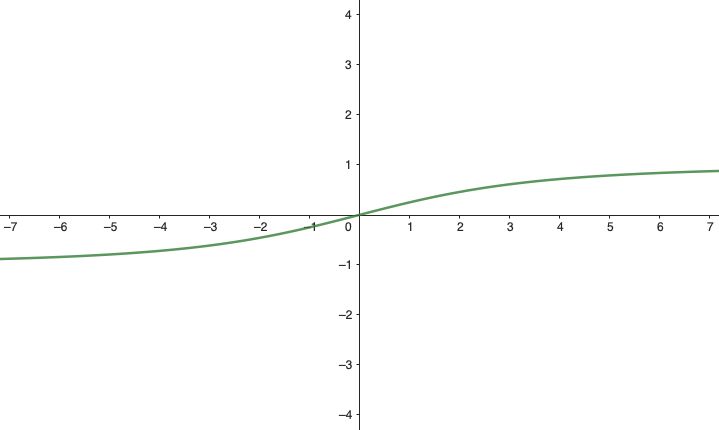
\includegraphics[width=0.98\textwidth]{gfx/grafica-normalizacion.png}
    \caption[Normalización utilizada con alfa como 15]{Normalización utilizada con alfa como 15.}\label{gfx:normalizacion}
\end{figure}

Se puede observar que a medida que \textit{x} crece, se acerca cada vez más a -1 o 1. Con un efecto similar, al usar muchas palabras en el sentimiento de \ac{VADER} se obtendrá una puntuación cercana a -1 o 1. Por lo tanto, el análisis de sentimientos de VADER funciona mejor en documentos cortos, como tweets o oraciones, no en documentos grandes.

\vspace{0.3cm}

Las características léxicas no es lo único que afecta al sentimiento de la oración. Existen otros elementos contextuales, como la puntuación, las mayúsculas y los modificadores que también imparten emoción. El análisis de sentimientos de \ac{VADER} los tiene en cuenta al considerar cinco heurísticas simples. El efecto de estas heurísticas se cuantifica, nuevamente, utilizando evaluadores humanos.

\vspace{0.3cm}

La primera heurística es la puntuación gramatical. Donde la oración \enquote{Me gusta}. expresa menos puntaje que \enquote{¡¡¡me gusta!!!}, esto es debido a que \ac{VADER} tiene en cuenta la cantidad de signos de exclamación y de interrogación que terminan la oración. \ac{VADER} primero calcula la puntuación de sentimiento de la oración. Si la puntuación es positiva, \ac{VADER} añade una cierta cantidad obtenida empíricamente por cada signo de exclamación (0,292) y signo de interrogación (0,18). Si la puntuación es negativa, entonces resta.

\vspace{0.3cm}

La segunda heurística es la capitalización. \enquote{INCREÍBLE actuación} es definitivamente más intenso que \enquote{increíble actuación}. Por ello, se aumenta o disminuye el puntaje de sentimiento de la palabra en 0.733, dependiendo de si la palabra es positiva o negativa, respectivamente. Esta característica no se ha implementado en mi proyecto, debido a que muchos tweets llevaban mayúsculas exclusivamente para llamar la atención y no para expresar sentimientos.

\vspace{0.3cm}

La tercera heurística es el uso de modificadores de grado. Por ejemplo, \enquote{muy lindo} y \enquote{más o menos lindo}. El efecto del modificador en la primera oración es aumentar la intensidad de lindo, mientras que en la segunda oración es disminuir la intensidad. \ac{VADER} mantiene un diccionario de refuerzo que contiene un conjunto de refuerzos y amortiguadores. Además, el efecto del modificador de grado también depende de su distancia a la palabra que está modificando. Las palabras más alejadas tienen un efecto intensificador relativamente menor sobre la palabra base. Un modificador al lado de la palabra suma o resta 0.293 al puntaje de sentimiento de la oración. Un segundo modificador de la palabra base suma o resta el 95\% de 0,293, y un tercero suma/resta el 90\%.

\vspace{0.3cm}

La cuarta heurística es el cambio de polaridad debido al \enquote{pero}. A menudo, \enquote{pero} conecta dos cláusulas con sentimientos contrastantes. El sentimiento dominante, sin embargo, es el último. Por ejemplo, \enquote{Te amo, pero ya no quiero estar contigo}. La primera frase \enquote{te amo} es positiva, pero la segunda \enquote{ya no quiero estar contigo}. es negativo y obviamente más dominante en cuanto al sentimiento. \ac{VADER} implementa un verificador de \enquote{pero}. Básicamente, todas las palabras sentimentales antes del \enquote{pero} tienen su valor reducido al 50\%, mientras que las que están después del \enquote{pero} aumentan al 150\%.

\vspace{0.3cm}

La quinta heurística es examinar el trigrama antes de una característica léxica cargada de sentimientos para captar la negación de la polaridad. Aquí, un trigrama se refiere a un conjunto de tres características léxicas. \ac{VADER} mantiene una lista de palabras negativas. La negación se captura multiplicando la puntuación de sentimiento de la característica léxica cargada de sentimiento por un valor determinado empíricamente -0,74.

\vspace{0.3cm}

Debido a todas estas características, la traducción del léxico inglés se ha realizado de una manera cuidadosa y selectiva (dejando las mismas puntuaciones que el léxico original), aunque se da por sentado que el léxico original tiene mayor capacidad de extraer los sentimientos. Sin embargo, la opción de traducir cada publicación iba a resultar mucho más costosa a la hora de ejecutarse. Primero la gran latencia de las múltiples traducciones que se puedan realizar y luego el limite de llamadas gratuitas diarias que claramente se van a traspasar.

\makeatletter
\let\orig@lstnumber=\thelstnumber

\newcommand\lstsetnumber[1]{\gdef\thelstnumber{#1}}
\newcommand\lstresetnumber{\global\let\thelstnumber=\orig@lstnumber}
\makeatother

\vspace{0.3cm}

\begin{lstlisting}[caption=Extracción de los sentimientos,          label={lst:listing-python},language=Python, mathescape=true]
def fetch_sentiments(query, lng, kw):

    if lng == 'es':
        analyzer = SentimentIntensityAnalyzerES()
    elif lng == 'uk':
        analyzer = SentimentIntensityAnalyzerUK()
    else:
        analyzer = SentimentIntensityAnalyzerEN()

    data: dict[str, list[list[float]]] = {
        'negative': [],
        'neutral': [],
        'positive': [],
    }

    try:
        if query:
            ppt = []
            for tweet in query:
                clean_txt = simple_clean(tweet.full_text)
                vader = round((analyzer.polarity_scores(clean_txt
                        ))['compound'], 4)
                y_axis = topic_relation(clean(clean_txt, lng),kw)
                popularity = ((tweet.retweet_count + 
                        tweet.favorite_count)*0.5)
                ppt.append(popularity)
                data = parse_data(data, vader, y_axis,popularity)$\lstsetnumber{\ldots}$
        $\lstresetnumber\setcounter{lstnumber}{45}$ 
        return data
    except Exception as e:

        print(e)
        return False
\end{lstlisting}

Como se ha explicado en la Historia de Usuario 11.1 (\ref{subs:sprint-8}) los sentimientos deberán estar representados en un gráfico. Por lo que los resultados proporcionados por \ac{VADER} pertenecerán al Eje X y la relación con las palabras clasificadas anteriormente será el Eje Y. Además, cada burbuja tiene un radio distinto, esto estará calculado conforme a la popularidad, es decir, si supera la popularidad media de la tendencia tendrá un radio más grande, pero también aumenta su radio si las coordenadas de las burbujas están muy cerca, para que no haya demasiadas repeticiones.

\vspace{0.3cm}

\begin{lstlisting}[caption=Extracción de las coordenadas de los sentimientos,          label={lst:extraccion-senti},language=Python, mathescape=true]
def parse_data(data, vader, y, ppt):
    if vader > 0.35:
        data['positive'].append([vader, y, ppt])
    elif vader < -0.35:
        data['negative'].append([vader, y, ppt])
    else:
        data['neutral'].append([vader, y, ppt])

    return data

def topic_relation(text, kw):
    suma = 0
    if len(text.split()):
        for k in kw:
            suma += text.split().count(k)
        relation = round(suma/len(text.split()), 4)
    else:
        relation = 0
    return relation

def fetch_sentiments(query, lng, kw):$\lstsetnumber{\ldots}$
    $\lstresetnumber\setcounter{lstnumber}{27}$
    m = np.max(ppt)
    a = round(np.average(ppt), 4)
    if m:
        for item in data.values():
            for k, i in enumerate(item):
                if i[2] > a:
                    i[2] = 2
                else:
                    i[2] = 1
                next = k + 1
    
                while next < len(item):
                    if round(i[0], 1) == round(item[next][0], 1)
                    and round(i[1], 1) == round(item[next][1],1):
                        i[2] = i[2] + 0.2
                        item.pop(next)
                    else:
                        next += 1
\end{lstlisting}

\subsection{Implementación de las Noticias}
La entidad de las noticias está compuesta por distintos valores comentados en la sección \ref{subsub:ent-noticias}. La estructuración de las noticias resulta tan sencilla como las que se han implementado anteriormente. Aunque la implementación tuvo varios cambios importantes.

\vspace{0.3cm}

\begin{lstlisting}[caption=Estructuración de las noticias,language=Python, mathescape=true]
# PARSING OBJECT WRAPPED
def parse_wrapped(item):

    date = item['date']
    image = item['image']
    summary = item['summary']
    title = item['title']
    url = item['url']
    source = item['source']

    values = {
        'date': date,
        'image': image,
        'summary': summary,
        'title': title,
        'url': url,
        'source': source
    }

    return Wrapped(**values)
\end{lstlisting}

Al empezar a implementar el código, pensé que la manera más sencilla de obtener información de noticias sería mediante una API. Aunque al usar distintas APIs sobre noticias, como \textit{News API} me di cuenta de que muchas noticias no estaban actualizadas, tenían errores en la descripción o el titulo y las APIs tenían por costumbre limitar drásticamente el número de peticiones por día.

\vspace{0.3cm}

Por ello tuve que cambiar el código y recurrir al scraping, una técnica utilizada para extraer información de sitios web. Para ello usé librerías como \textit{BeautifulSoup} o \textit{newspaper}, bibliotecas de Python para analizar documentos HTML y extraer de ellas información que resulte relevante.

\vspace{0.3cm}

Primero se descarga la búsqueda de noticias relevantes mediante el recurso XML de Google News. Esto se hace mediante los tópicos que se han extraído anteriormente y la biblioteca \textit{BeautifulSoup}, de esta manera las noticias serán mucho más refinadas. Además, siempre se intenta conseguir tres noticias diferentes y actuales, limitando la búsqueda por fecha.

\vspace{0.3cm}

Otro punto diferencial en la herramienta scraping y la API, es que con la herramienta scraping se conseguían artículos muchos más actuales y a la vez diferentes. Esto es debido a que al descargar artículos mediante la API solamente se podía condicionar el parámetro de búsqueda mediante la relevancia o actualidad, por lo que muchos artículos se podían repetir o quedaban desfasados. Gracias al scraping se pueden conseguir artículos recientes y a la vez relevantes, combinado los parámetros de búsqueda en Google News. Además, el problema de los artículos repetidos quedaba solucionado al usar un buscador más sotisficado que el de la API News.

\vspace{0.3cm}

\begin{lstlisting}[caption=Extracción de las noticias,language=Python, mathescape=true]
# GETTING ARTICLES
def get_everything(query, code, lang):
    # Getting the XML Content from Google News
    # An example: #https://news.google.com/rss/search?q=Riot+when:1d&hl=es&gl=ES&ceid=ES:es
    query = urllib.parse.quote(query.encode('utf8'))
    BASE_URL = f"https://news.google.com/rss/search?q={query}&hl={lang}&gl={code}&ceid={code}:{lang}"
    xml_content = requests.get(BASE_URL).content
    soup = BeautifulSoup(xml_content, features="xml")
    g_items = soup.find_all("item")

    if len(g_items) > 0:
        # Google Articles with poor info and not parsed yet
        g_articles = []
        for item in g_items:
            article = {}
            article["link"] = item.find("link").text
            article["title"] = item.find("title").text
            article["publisher"] = item.find("source").text
            article["published_date"] = item.find("pubDate").text
            g_articles.append(article)

        # Google with more info and parsed
        articles: list[dict[str, str]] = []
        cont = 0
        while len(articles) != 3 and cont < len(g_articles):
            article_info = get_article_info(g_articles[cont],
                        lang)
            if article_info:
                articles.append(article_info)
            cont += 1
        if len(articles) == 3:
            return articles
            
    return False
\end{lstlisting}

Al estar descargando información de Google News lo hacemos desde la ruta \textit{rss}. \ac{RSS} contiene un resumen de las actualizaciones de un sitio web y está escrito en XML. Una de las etapas más importantes del análisis de archivos XML es la búsqueda de etiquetas. Hay varias formas de hacer esto, mediante nombres o relaciones.

\vspace{0.3cm}

Al estar en recopilando información de una página simple y estática, como son los artículos de Google News se ha utilizado la extracción de información mediante nombres. La función de \textit{find} recibe el nombre de la etiqueta que desea obtener y devuelve un objeto BeautifulSoup de la etiqueta si encuentra uno, de lo contrario, devuelve \textit{None}.

\vspace{0.3cm}

De esta manera se puede realizar un bucle de todos los artículos relacionados con la tendencia. Consiguiendo información importante, como su enlace, el título, la editorial y la fecha de publicación.

\vspace{0.3cm}

Gracias a los artículos recopilados y sus enlaces correspondientes, podemos proseguir consiguiendo información relevante como una imagen de portada o la descripción.

\vspace{0.3cm}

\begin{lstlisting}[caption=Extracción de la información de las noticias,language=Python, mathescape=true]
# GETTING ARTICLES
def get_article_info(item, lang):
    user_agent = 'Mozilla/5.0 (Macintosh; Intel Mac OS X 10.15; rv:78.0) Gecko/20100101 Firefox/78.0'
    config = Config()
    config.browser_user_agent = user_agent
    config.request_timeout = 100
    config.MAX_TEXT = 500
    config.language = lang
    config.number_threads = 100
    a = Article(item["link"], language=lang, config=config)
    
    try:
        a.download()
        a.parse()
        date = parser.parse(item["published_date"])
        date_parsed = date.strftime("Date: %y-%m-%d Time: %H:%M")
        values = {
            'date': date_parsed,
            'image': a.top_image,
            'summary': a.text,
            'title': a.title,
            'url': item["link"],
            'source': item["publisher"]
        }
        if values["title"] and values["summary"] 
        and len(values["summary"].split()) > 20 
        and values["title"] != "Are you a robot?":
            return values
        else:
            return False
            
    except ArticleException as ae:
        print(ae)
        return False
        
    except Exception as e:
        print(e)
        return False
\end{lstlisting}

En esta sección de código, en vez de usar la biblioteca BeautifulSoup, se ha utilizado \textit{Newspaper3k}. Las ventajas de ello es que, la biblioteca Newspaper3k también puede realizar funciones más avanzadas, como descubrir fuentes RSS, buscar URL de artículos de una fuente de noticias principal e incluso extraer varios subprocesos si tiene que buscar más de un artículo. Además, termina siendo más conveniente al extraer información de sitios web diferentes.

\vspace{0.3cm}

Se ha establecido un gran tiempo para la conexión, para asegurar la descarga del articulo y su información, debido a esto el proceso de recopilación de datos sobre la tendencia resulta muy costoso. Aunque gracias al multiprocesamiento, se ha podido realizar las descargas de manera no secuencial y aligerar el proceso.

\vspace{0.3cm}

Después de añadir otras configuraciones como un \textit{header} para poder acceder a la página web sin limitaciones, se recopilan los diferentes datos y se estructuran de una manera conveniente. Además, pasan por validación por si la información recopilada no tiene sentido, en este caso la validación es bastante simple aunque efectiva. La descripción debe tener al menos 20 palabras, debe existir un título y que no sea \enquote{Are you a robot?}. La última validación es debido a que algunas páginas web comprueban cuidadosamente las peticiones que se hacen por estos métodos y devuelven esa información, en vez del articulo.

\subsection{Implementación del Servidor}
Anteriormente se ha descrito las diferentes implementaciones sobre las entidades, su estructuración y extracción de datos. Dichas implementaciones se encuentran en la carpeta \textit{app}, mientras que todo lo relacionado con el servicio del servidor se encuentra en el directorio \textit{backend}. No entraré en mucho detalle en la implementación de las clases o rutas, ya que se han explicado en la sección de diseño (\ref{ch:diseño}). Aunque interferiré en el modelo \textit{Country} y su obtención.

\vspace{0.3cm}

\begin{lstlisting}[caption=Modelo \textit{Country} y ejemplo de ruta,language=Python, mathescape=true]
class Country(BaseModel):
    id: str = Field(default_factory=uuid.uuid4, alias="_id")
    pais: str = Field(...)
    dia: str = Field(...)
    tendencias: List[Trend] = Field(...)

    class Config:
        allow_population_by_field_name = True
        schema_extra = {
            "example": {
                "_id": "066de609-b04a-4b30-b46c-32537c7f1f6e",
                "pais": "Spain",
    $\lstsetnumber{\ldots}$
    $\lstresetnumber\setcounter{lstnumber}{0}$

@router.get("/{name}/{date}", response_description=
    "Get a single country by the name and date",
    response_model=Country)
def find_country(name: str, date: str, request: Request):
    if (country := request.app.database["countries"].find_one(
    {"pais": name, "dia": date})) is not None:
        country["tendencias"] = list(
            filter(itemgetter("wrappeds"),
            country["tendencias"]))[:10]
        return country

    raise HTTPException(status_code=status.HTTP_404_NOT_FOUND,
                        detail=f"Country with the name {name} 
                        and date {date} not found")
\end{lstlisting}

La ruta devuelve un objeto bajo el modelo de \textit{Country} mediante la fecha y el nombre del país, tal y como se ha explicado en la sección de diseño de interacción de rutas (diagrama \ref{gfx:diagrama-itr4}). Todas las demás rutas y entidades tienen un comportamiento parecido. La peculiaridad de esta ruta es que filtra diez tendencias que tengan el objeto de noticias o \textit{wrappeds}, para no mostrar tendencias vacías.

\section{Implementación Front-end}
La implementación de la capa de \textit{Front-end} se localiza bajo el directorio \textit{front-end}, la estructura de la aplicación de Vue sigue las buenas prácticas conteniendo archivos correspondientes en cada directorio relevante a la aplicación, es decir, se han separado en \textit{assets}, \textit{components}, \textit{router}, \textit{styles} y la carpeta \textit{public}.

\subsection{Implementación Principal}
La primera implementación de código que se estudiará será la vista principal descrita anteriormente en la sección \ref{subs:vista-principal}. Cabe mencionar que no se podrá estudiar todo el código, debido a que incluir todas las reglas de diseño CSS y la estructura HTML complicarían la lectura y su propia comprensión. Aunque indagaré en las diferencias más destacables.

\vspace{0.3cm}

La estructura de un archivo Vue se compone de tres apartados esenciales, el primer apartado llamado \textit{template} contiene la implementación HTML, el segundo llamado \textit{script} contendrá implementaciones de JavaScript y por último \textit{style} incluirá implementaciones de diseño.

\vspace{0.3cm}

\begin{lstlisting}[caption=Secciones de Vue,language=Python, mathescape=true]
<template>$\lstsetnumber{\ldots}$
        $\lstresetnumber\setcounter{lstnumber}{120}$
          <div class="flex overflow-x-auto gap-6 snap-x snap-mandatory sm:snap-normal before:shrink-0 before:w-[20%] sm:before:w-[0%] after:shrink-0 after:w-[20%] sm:after:w-[0%] sm:horizontal sm:pb-14 pb-5">
            <div
              v-if="articulos.popularity"
              class="basis-4/5 sm:basis-3/12 xl:basis-2/12 shrink-0 snap-center sm:snap-align-none shadowdrop"
            >
              <GraphViewer
                :array-popularity="articulos.popularity.volume"
                :array-hours="articulos.popularity.hour_popularity"
                :avarage-popularity="articulos.popularity.avarage_popularity"
                :peak-popularity="articulos.popularity.peak_popularity"
                :num="1"
                :rank="index+1"
                :url="encondeURL(articulos.name)"
              />
            </div>$\lstsetnumber{\ldots}$
                    $\lstresetnumber\setcounter{lstnumber}{163}$
</template>

<script>
import axios from 'axios';$\lstsetnumber{\ldots}$
$\lstresetnumber\setcounter{lstnumber}{270}$
export default {
  components: {
    CardViewer,
    GraphViewer,
    MapViewer,
    BubbleViewer,
  },$\lstsetnumber{\ldots}$
$\lstresetnumber\setcounter{lstnumber}{410}$
</script>

<style>$\lstsetnumber{\ldots}$
$\lstresetnumber\setcounter{lstnumber}{425}$
.truncador-title {
  overflow: hidden;
  display: -webkit-box;
  -webkit-box-orient: vertical;
  -webkit-line-clamp: 2;
  -webkit-margin-collapse: discard;
}$\lstsetnumber{\ldots}$
$\lstresetnumber\setcounter{lstnumber}{570}$
</style>

\end{lstlisting}

En la sección \textit{template} de esta vista se encuentra toda la estructura HTML de la página y llamadas a otros componentes. Gracias a funciones Vue se ha podido implementar bucles o funciones directamente en dicha estructura. Un ejemplo de ello es el \textit{v-if} o \textit{v-for} los cuales renderizan contenido mediante condiciones o listas. La renderización de listas fue algo esencial a la hora de renderizar un \ac{JSON} devuelto de la base de datos.

\vspace{0.3cm}

Luego, en la sección de \textit{script} se implementa la parte programable. En el caso de la vista principal se realizan llamadas a la base de datos justo en la creación de la página web, esto es debido a que el contenido se cargue justo al inicio de la creación de la página web, sin tener que esperar a la carga de todos los componentes necesarios como se puede ver en el esquema posterior.

\begin{figure}[H]
    \centering
    \myfloatalign
    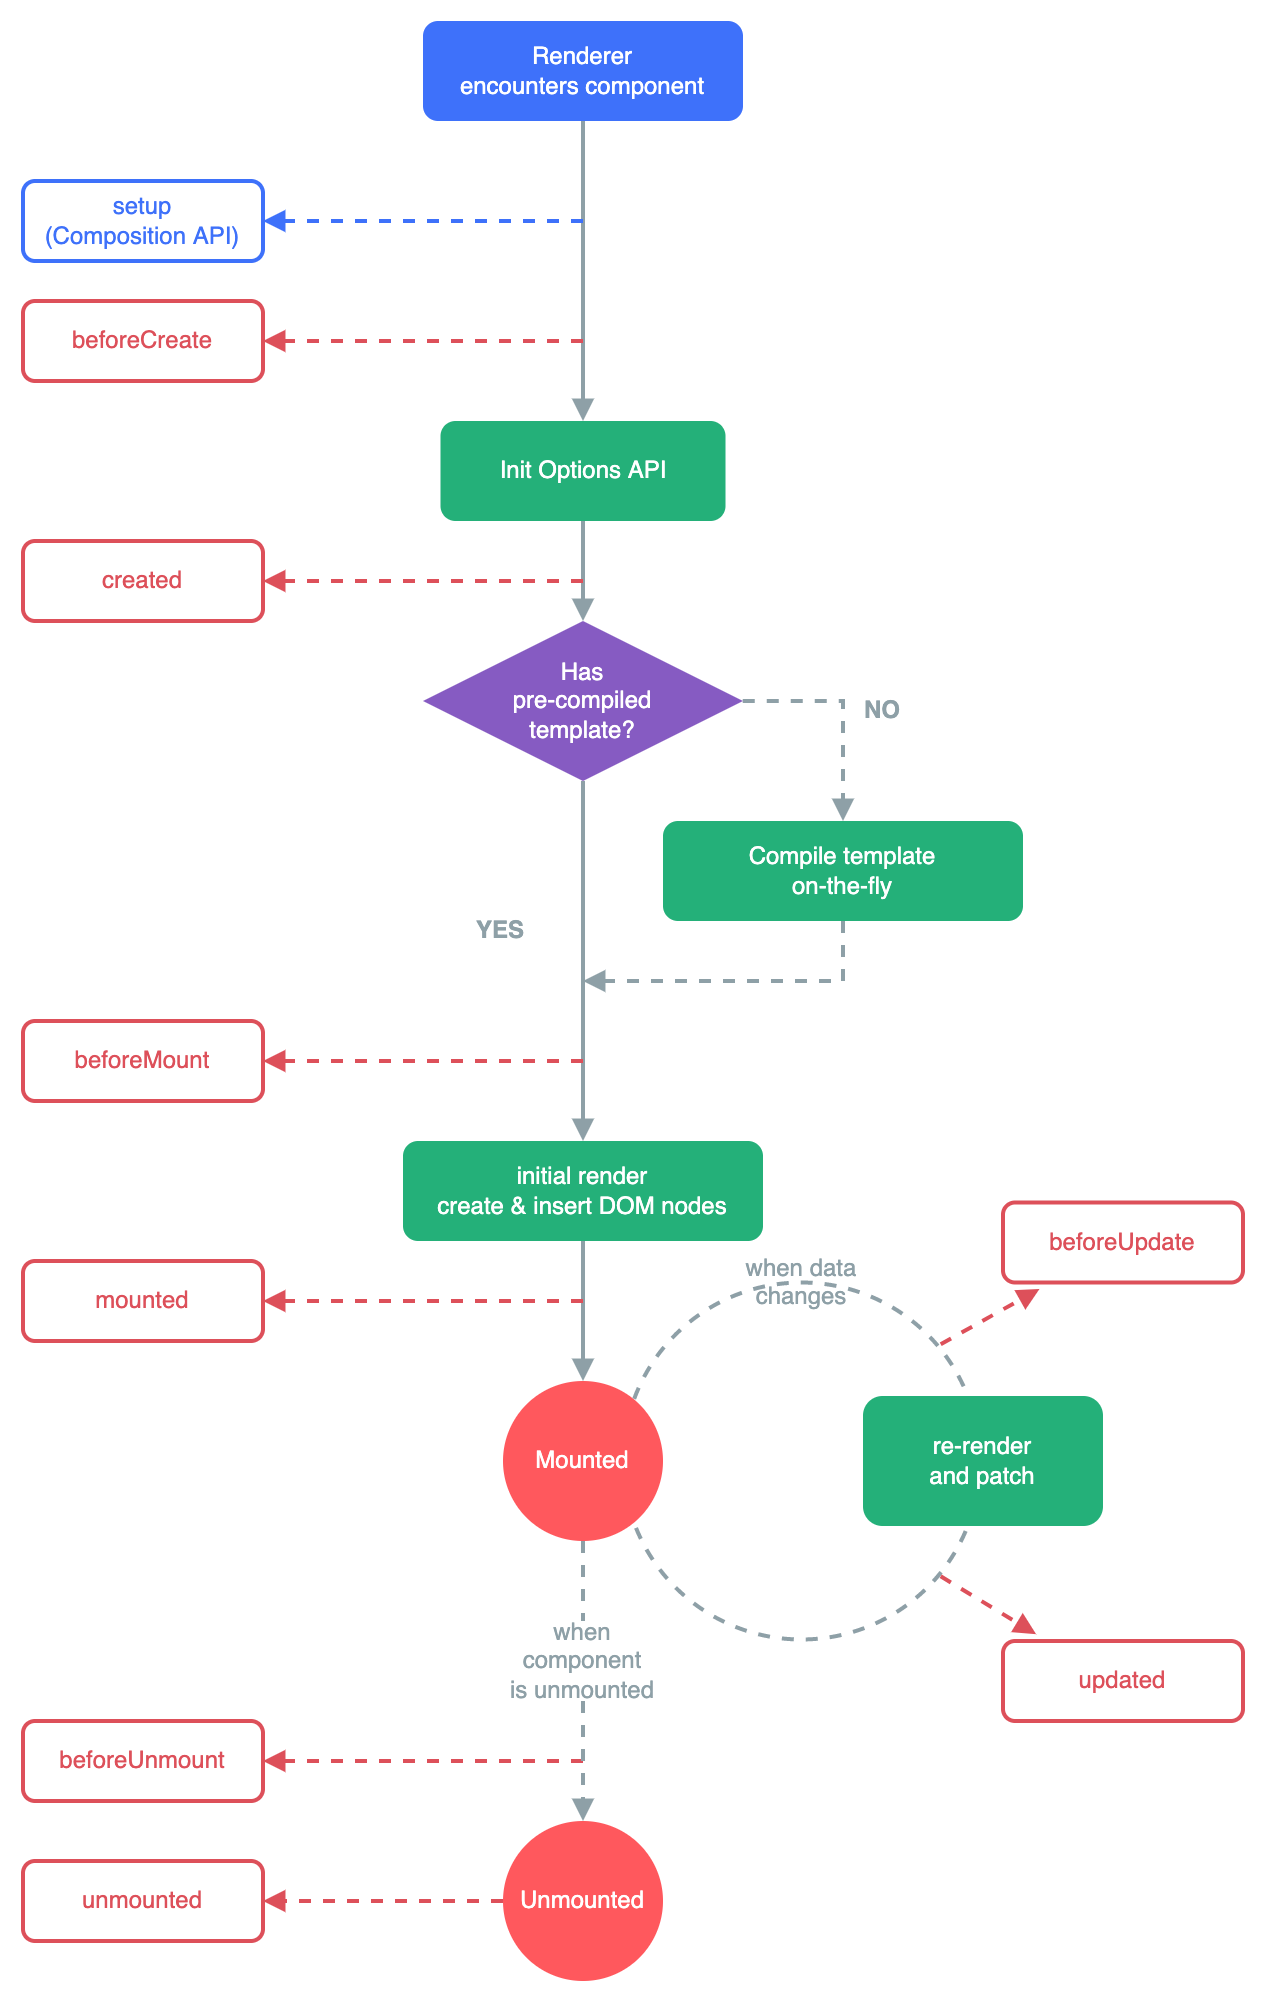
\includegraphics[width=0.82\textwidth]{gfx/lifecyclevue.png}
    \caption[Ciclo de vida de una aplicación Vue]{Ciclo de vida de una aplicación Vue \cite{vue-life}.}\label{gfx:lifecyclevue}
\end{figure}

El código mostrado es una versión simplificada, con el objetivo de facilitar la comprensión. Lo importante del código es que se ha implementado un manejo de errores y la creación de contenido de la página dependiendo de la URL que se haya introducido.

\vspace{0.3cm}

\begin{lstlisting}[caption=Funciones de carga de contenido en Vue,language=Python, mathescape=true]
async created() {
    await this.fetch();
},
methods: {
    async fetch() {
      this.loading = true;
      try {
        let data = {};
        if (this.route.query.name and this.route.query.query) {
          data = await axios.get((`{SEARCHTRENDINGENDPOINT}`));
        } else { data = await axios.get((`{TRENDINGENDPOINT`));}
        if (data.status === 200 and data.data.
            tendencias[0].wrappeds) {
          this.wrapped = data.data.tendencias;
          this.loading = false;
          this.error = false;
        } else {
          this.country = 'Spain';
          this.date = this.dateString(new Date());
          this.alert('There was an error trying to load (...)');
        }
      } catch (error) {
        this.country = 'Spain';
        this.date = this.dateString(new Date());
        this.alert('Right now it looks like the web is (...)');
        console.log(error);
      }
    },
},
\end{lstlisting}

Otra sección a destacar el el diseño. La implementación de esta sección tuvo el mismo o incluso más arduo trabajo que las demás, primero al querer tener un diseño original y que funcionase en todos los dispositivos, se han implementado muchísimas reglas en CSS, entre ellas reglas de medida o consultas de medio para cambiar toda la visualización de contenido dependiendo de la medida del dispositivo. 

\vspace{0.3cm}

Esto es debido a que se ha querido que se viera de una manera óptima sin sacrificar la visibilidad del contenido. Por ello se ha recurrido a herramientas como el truncamiento en CSS. Luego otro de los detalles del diseño es que las sombras varían dependiendo del navegador, debido al rendimiento que tienen sobre estos. El navegador Chrome llega a funcionar muy bien con la opción \textit{filter()} de CSS, pero sin embargo Safari no. También hay que tener en cuenta las personas que tengan el zoom activado en el teléfono y adaptar también su contenido, incluso pantallas gigantes o extremadamente pequeñas, todo esto hace que el diseño pueda ser debidamente \textit{responsive}.

\vspace{0.3cm}

Otro detalle, a parte de las sombras, es que, en los dispositivos no móviles, se han implementado animaciones de \textit{hover}. Estas animaciones levantan y oscurecen ligeramente la carta o módulo cada vez que el ratón pasa por encima, facilitando así su visualización.

\vspace{0.3cm}

También se han seguido las buenas prácticas y se ha respetado el contraste de los colores para la una lectura más fácil de los enlaces web o el propio contenido de la página. Además, se han usado varios \textit{svg} con formas de ola, para que la página sea más agradable a la vista.

\vspace{0.3cm}

\begin{lstlisting}[caption=Detalles de la implementación del diseño,language=Python, mathescape=true]
@media (min-height: 550px) {
  contenido {
    height: 10rem;
  }

  .truncador {
    overflow: hidden;
    display: -webkit-box;
    -webkit-box-orient: vertical;
    -webkit-line-clamp: 5;
    -webkit-margin-collapse: discard;
  }$\lstsetnumber{\ldots}$
$\lstresetnumber\setcounter{lstnumber}{37}$
}

/* Safari 10.1+ */
@media not all and (min-resolution:.001dpcm) { @media {
  .shadowdrop {
    filter: none;
    -webkit-filter: none;
    -moz-filter:  none;
    -ms-filter:  none;
    -o-filter: none;
    box-shadow: rgba(0, 0, 0, 0.03) 0px 15px 7px -7px;
  }
}}
\end{lstlisting}

\subsection{Implementación de la Popularidad}
El código implementado en esta sección se refiere a la subvista popularidad explicada en la sección \ref{subs:vista-popu}. Las principales diferencias de implementación en este módulo es la implementación de diferentes funciones en el \textit{template} de la vista y también la propia implementación del gráfico, ya que es una librería que requiere mucha personalización para poderse visualizar adecuadamente.

\vspace{0.3cm}

\begin{lstlisting}[caption=Diferencias destacables de la implementación de la popularidad,language=Python, mathescape=true]
<ul class="text-sm contenido-stats text-ellipsis overflow-hidden">
  <li class="py-0.5 pt-1">
    - First data at {{ encondeHour(arrayHours[0]) }}.
  </li>
  <li class="py-0.5">
    - Last data at
    {{ encondeHour(arrayHours[arrayHours.length - 1]) }}.
  </li>
  <li class="py-0.5">
    - Peak popularity is {{ peakPopularity.toLocaleString('en-US') }}.
  </li>
  <li class="py-0.5 pb-1">
    - Average popularity is {{ avaragePopularity.toLocaleString('en-US') }}.
  </li>
</ul>$\lstsetnumber{\ldots}$
$\lstresetnumber\setcounter{lstnumber}{62}$
chartOptions: {
    chart: {
      type: 'area',
      toolbar: {
        show: false,
      },
      zoom: {
        enabled: false,
      },
      animations: { enabled: false },
    },
    xaxis: {
      type: 'datetime',
      categories: this.arrayHours,
      labels: {
        format: 'HH:mm',
        },$\lstsetnumber{\ldots}$
        $\lstresetnumber\setcounter{lstnumber}{94}$
        markers: {
          size: 3,
        },
      },
\end{lstlisting}

Las horas en este caso se guardan en formato JavaScript y se transforman en objeto \textit{date} al implementarlo en el código Vue. Además, se ha respetado las horas locales de cada país como se puede ver en el código.

\vspace{0.3cm}

En el siguiente ejemplo de visualización, se ha usado el navegador de Chrome bajo la premisa de simular la vista de un iPhone SE (un teléfono bastante compacto). El contenido que se puede visualizar es el descenso de popularidad que tuvo la tendencia \textit{Joji}. Podemos ver cómo empezó siendo popular sobre la madrugada, pero que poco a poco fue decayendo. En el día de 5 de noviembre, se encuentra en la octava posición del top 10 tendencias más populares de España. El valor del volumen de publicaciones, es decir el número de veces que se ha mencionado la tendencia fue de 86,748 como máximo y 59,957 de media.

\begin{figure}[H]
    \centering
    \myfloatalign
    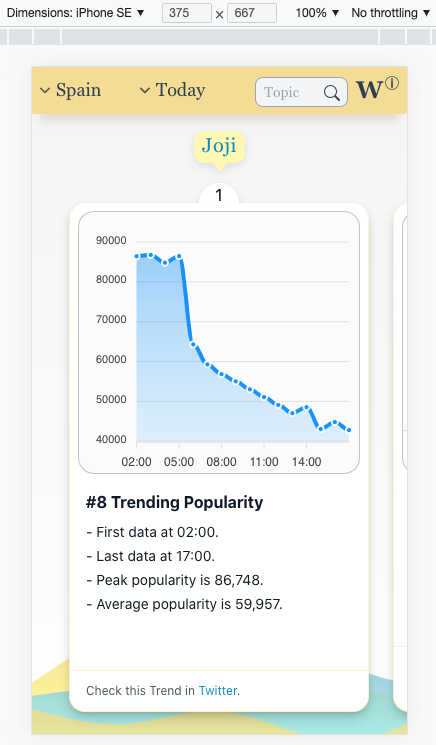
\includegraphics[width=0.75\textwidth]{gfx/ejemplo2.png}
    \caption[Ejemplo de tendencia, vista de popularidad]{Ejemplo de tendencia, vista de popularidad.}\label{gfx:ejemplo2}
\end{figure}

\subsection{Implementación de las \textit{Keywords}}
El código implementado en esta sección se refiere a la subvista \textit{keywords} explicada en la sección \ref{subs:vista-key}. En cuanto a las principales diferencias, es la cantidad de código que ha requerido la implementación de la personalización del gráfico.

\vspace{0.3cm}

\begin{lstlisting}[caption=Diferencias destacables de la implementación de las keywords,language=Python, mathescape=true]
series: this.arrayCount,
chartOptions: {
chart: {
  type: 'radialBar',
  toolbar: {
    show: false,
  },
  animations: { enabled: false },
  sparkline: {
    enabled: true,
  },
},
colors: [
  '#008FFB',
  '#00E396',
  '#FEB019',
  '#FF4560',
  '#775DD0',
  '#5DABD0',
],
plotOptions: {
  radialBar: {
    offsetY: -5,
    startAngle: 0,
    endAngle: 360,
    hollow: {
      margin: 5,
      size: '0%',
      background: 'transparent',
    },
$\lstsetnumber{\ldots}$
$\lstresetnumber\setcounter{lstnumber}{0}$
\end{lstlisting}

Los colores y sombras han sido definidos manualmente, al igual que la posición del gráfico y el etiquetado de sus datos.

\vspace{0.3cm}

En el siguiente ejemplo podemos visualizar el contexto de la tendencia. Obviamente el nombre de la tendencia es la palabra que más se repite en las publicaciones, se ha repetido 99 veces en los 100 tweets recopilados. Para entender la situación podemos ver las palabras más repetidas y los \textit{keywords}, la información que nos dan es «Album De Joji», «Die For You» y «Nuevo Disco». Al parecer Joji es un cantante o al menos una persona famosa, que ha sacado un disco o álbum nuevo llamado "Die For You".

\begin{figure}[H]
    \centering
    \myfloatalign
    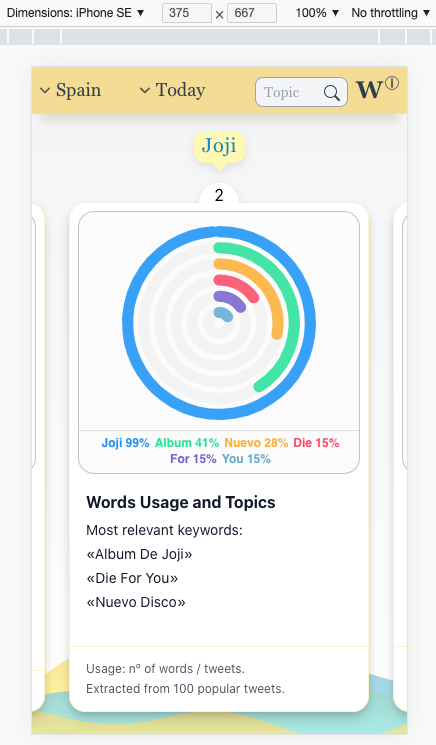
\includegraphics[width=0.75\textwidth]{gfx/ejemplo3.png}
    \caption[Ejemplo de tendencia, vista de \textit{keywords}]{Ejemplo de tendencia, vista de \textit{keywords}.}\label{gfx:ejemplo3}
\end{figure}

\subsection{Implementación de los Sentimientos}
El código implementado en esta sección se refiere a la subvista sentimientos explicada en la sección \ref{subs:vista-senti}. Aquí también destaca la implementación la personalización del gráfico, aunque también hay funciones que requieren explicación.

\vspace{0.3cm}

Todos los ejes, el marco o las propias burbujas han tenido su implementación de posición, color y grosor de trazado. Además, el lienzo en el que se pinta es algo más grande que la notación del etiquetado, esto es debido a que se pretende que se visualice mejor la gráfica y no se corten las burbujas.

\vspace{0.3cm}

\begin{lstlisting}[caption=Diferencias destacables de la implementación de los sentimientos,language=Python, mathescape=true]
xaxis: {
  min: -1,
  max: 1,
  tickAmount: 1,
  type: 'numeric',
  position: 'bottom',
  decimalsInFloat: 0,
  labels: {
    offsetY: -4,
    style: {
      fontSize: '11px',
    },
  },
  axisBorder: {
    show: false,
  },
  axisTicks: {
    show: false,
  },
  title: {
    text: 'Compound',
    offsetY: -22,
    style: {
      fontSize: '12px',
      fontWeight: 350,
    },
  },
},
$\lstsetnumber{\ldots}$
$\lstresetnumber\setcounter{lstnumber}{132}$
percentageSentiment(array, arrayA, arrayB) {
  let suma = 0;
  let val = 0;
  array.forEach((item) => {
    suma += item[2];
  });
  val = suma;
  arrayA.forEach((item) => {
    suma += item[2];
  });
  arrayB.forEach((item) => {
    suma += item[2];
  });
  return (Math.round((val / suma) * 100));
},
\end{lstlisting}

El porcentaje se calcula en torno al radio de la burbuja, ya que no tiene sentido calcular la cantidad de burbujas porque como se ha explicado en la sección de su implementación (\ref{lst:extraccion-senti}) se eliminan las que tienen coordenadas muy similares.

\vspace{0.3cm}

En el ejemplo siguiente, del cantante Joji, la mayoría de las publicaciones tienen que ser positivas debido a los seguidores de esta persona, al comprobarlo vemos que efectivamente el 56\% son publicaciones positivas. También puede haber publicaciones negativas o neutras, tal como análisis de críticos que no expresan una opinión o personas a las que no les ha gustado. Claramente también puede haber errores, ya que la extracción del sentimiento no es cien por cien precisa, aunque se puede ver que el sentimiento global es acertado.

\begin{figure}[H]
    \centering
    \myfloatalign
    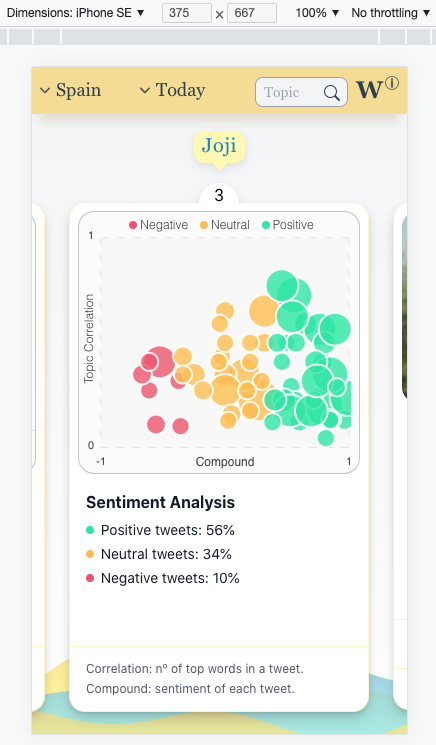
\includegraphics[width=0.75\textwidth]{gfx/ejemplo4.png}
    \caption[Ejemplo de tendencia, vista de sentimientos]{Ejemplo de tendencia, vista de sentimientos.}\label{gfx:ejemplo4}
\end{figure}

También se puede comprobar por tweets o publicaciones específicas, ya que cada burbuja es una:

\vspace{0.3cm}

\begin{quotation}
		\textit{"lo siento jefe hoy no puedo trabajar el album de joji me ha puesto triste"}
\end{quotation}
Puntuación: -0.7061

\vspace{0.4cm}

Podemos ver y comprobar la publicación en la propia plataforma.

\begin{figure}[H]
    \centering
    \myfloatalign
    
\includegraphics[width=0.95\textwidth]{gfx/twit1.png}
    \caption[Ejemplo de tweet (1)]{Ejemplo de tweet (1).}\label{gfx:twit1}
\end{figure}

\vspace{0.3cm}

\begin{quotation}
		\textit{"hoy es un buen dia porque joji saco un nuevo album con musica muy buena, asi que, buenos dias; escuchen a joji, es arte."}
\end{quotation}
Puntuación: 0.902

\vspace{0.4cm}

El sentimiento en este caso también es justificado. Podemos ver y comprobar la publicación en la propia plataforma.

\begin{figure}[H]
    \centering
    \myfloatalign
    
\includegraphics[width=0.95\textwidth]{gfx/twit2.png}
    \caption[Ejemplo de tweet (2)]{Ejemplo de tweet (2).}\label{gfx:twit2}
\end{figure}

\vspace{0.3cm}

\begin{quotation}
		\textit{"toca llorar toda la noche escuchando el nuevo album de joji en loop"}
\end{quotation}
Puntuación: -0.34

\vspace{0.3cm}

El sentimiento en este caso también es justificado, aunque obviamente es una publicación sarcástica, algo que la herramienta de extracción no entendería.

\vspace{0.3cm}

Lo bueno de comprobar estas publicaciones que las imágenes u otros elementos como los \textit{hashtags} no interfieren en el análisis de sentimientos. Además, se recogen publicaciones con mucha interacción, tal y como lo hemos especificado en el algoritmo.

\vspace{0.1cm}

\begin{figure}[H]
    \centering
    \myfloatalign
    
\includegraphics[width=0.81\textwidth]{gfx/twit3.png}
    \caption[Ejemplo de tweet (3)]{Ejemplo de tweet (3).}\label{gfx:twit3}
\end{figure}

\subsection{Implementación de las Noticias}
El código implementado en esta sección se refiere a la subvista \textit{keywords} explicada en la sección \ref{subs:vista-noti}. En cuanto a las principales diferencias, no destaca mucho en la implementación, ya que solo tiene que mostrar valores proporcionados de la página web, pero destaca en el diseño.

\vspace{0.3cm}

Las animaciones y otros detalles parten de esta vista. También existe una función que, ante un fallo de carga de imagen, provee una imagen por defecto para las noticias.


\vspace{0.3cm}

\begin{lstlisting}[caption=Diferencias destacables de la implementación de las noticas,language=Python, mathescape=true]
import img from '../assets/img_news.jpg';
export default {
  methods: {
    replaceByDefault(e) {
      e.target.src = img;
    },
  },
$\lstsetnumber{\ldots}$
$\lstresetnumber\setcounter{lstnumber}{122}$
@media (hover: hover) and (pointer: fine) {
  .animation:hover {
    --tw-translate-y: -0.5rem /* -8px */;
    transform: translate(var(--tw-translate-x), var(--tw-translate-y))
      rotate(var(--tw-rotate)) skewX(var(--tw-skew-x)) skewY(var(--tw-skew-y))
      scaleX(var(--tw-scale-x)) scaleY(var(--tw-scale-y));
  }
  .animation-shadow:hover {
    --tw-shadow: 0 20px 25px -12px rgb(0 0 0 / 0.35);
    --tw-shadow-colored: 0 20px 25px -12px var(--tw-shadow-color);
    box-shadow: var(--tw-ring-offset-shadow, 0 0 #0000),
      var(--tw-ring-shadow, 0 0 #0000), var(--tw-shadow);
  }
}
\end{lstlisting}

Hay tres noticias bastante parecidas. Las tres anuncian el nuevo álbum, a lo mejor también información sobre sus conciertos o donde poder escucharlo.

\begin{figure}[H]
    \centering
    \myfloatalign
    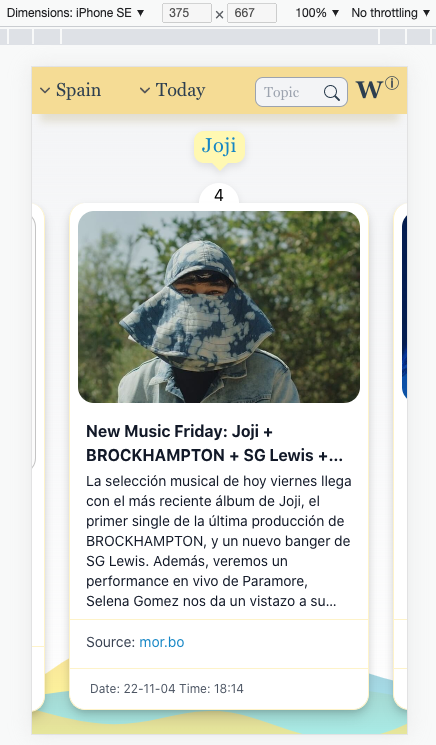
\includegraphics[width=0.75\textwidth]{gfx/ejemplo5.png}
    \caption[Ejemplo de tendencia, vista de noticias]{Ejemplo de tendencia, vista de noticias.}\label{gfx:ejemplo5}
\end{figure}

La noticia presenta un titulo, descripción y fotografía explicativa. La fotografía es del cantante Joji. Se puede acceder a dicho articulo mediante el enlace de la editorial o directamente pulsando sobre la foto.

\begin{figure}[H]
    \centering
    \myfloatalign
    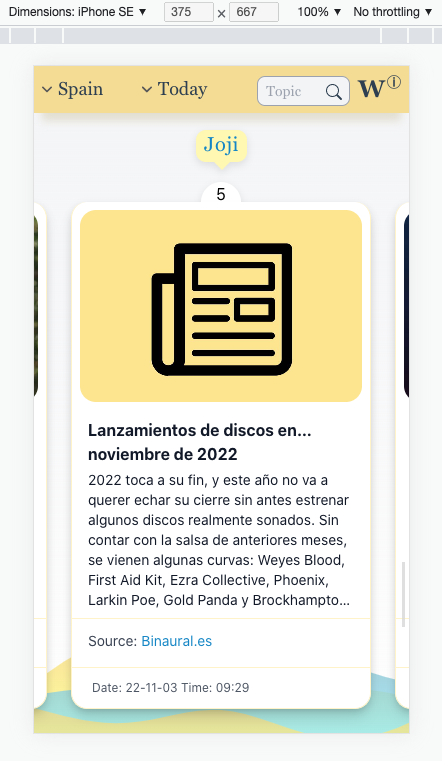
\includegraphics[width=0.75\textwidth]{gfx/ejemplo6.png}
    \caption[Ejemplo de tendencia, vista de noticias por defecto]{Ejemplo de tendencia, vista de noticias por defecto.}\label{gfx:ejemplo6}
\end{figure}

La búsqueda por tópicos funcionaria de la misma manera. Como ultima mención, la implementación de errores fue implementada tal cual descrita en la sección \ref{gfx:boceto-error}. El mensaje de la alerta cambia dependiendo del error ocurrido, para que el usuario tenga conciencia de cuál fue el problema. 
	%\chapter{Deducciones y resultados}\label{ch:deducciones}
%************************************************

\section{Conclusiones y pruebas de prestaciones}
Este trabajo, aunque solamente tenga un objetivo, el cual es enseñar una pequeña visión del mundo en un instante dado, ha demostrado aparte de cumplir dicho objetivo, ser una aplicación rígida y estar construida de una manera actual.

\vspace{0.3cm}

Aparte de haber demostrado la capacidad de poder programar el funcionamiento de la aplicación, se ha demostrado la competencia en la construcción del planteamiento, de la arquitectura y la propia estructura de la aplicación. Todo ello gracias al aprendizaje llevado a cabo en el grado de ingeniería de informática.

\vspace{0.3cm}

Aunque al hacer diferentes pruebas de prestaciones con herramientas como JMeter o benchmarks de distintas páginas web, me he podido dar cuenta de las limitaciones que ha supuesto usar distintas herramientas como \textit{framework} Vue o las plataformas gratuitas de servicio.

\vspace{0.3cm}

Las plataformas, al ser gratuitas funcionan con más limitaciones. La latencia puede llegar a ser más grande ya que te limitan el uso a los servidores gratuitos y además los servidores están separados en distintas máquinas, cada una conectada en una región diferente.

\vspace{0.3cm}

Al estar usando Vue me pude dar cuenta de las limitaciones que supone usar un DOM virtual, al tener mucha carga de JavaScript, debido a los diferentes gráficos, el tiempo de la carga de la página se hace mayor. Esto no pasaría en un \textit{framework} estático como Svelte, aunque otra manera de arreglarlo sería construir componentes \textit{skeleton} o esqueleto, los cuales cargan la estructura de toda la página y solo cambian los componentes necesarios. Intenté implementar la segunda opción, pero he tenido bastantes fallos debido a la librería de áreas y gráficas, y porque dicho componente esqueleto sigue aún en fase de beta.

\vspace{0.3cm}

El escenario supuesto de la herramienta de Jmeter consiste en analizar el rendimiento de la página donde 5 usuarios interaccionan durante un intervalo de tiempo predeterminado, en este caso ocho minutos.

\begin{figure}[H]
    \centering
    \myfloatalign
    \includegraphics[width=1\textwidth]{gfx/prueba1.png}
    \caption[Prueba de prestaciones con Jmeter]{Prueba de prestaciones con Jmeter.}\label{gfx:prueba1}
\end{figure}

Al analizar el rendimiento nos damos cuenta de varias cosas que ya hemos comentado. Primero, hay que tener en cuenta que los errores son debido a la carga de contenido externo, en este caso imágenes de los artículos de las noticias. Esto se puede arreglar si descargamos las imágenes en vez de cargar el contenido de fuera. En general el rendimiento de la página es aceptable para la carga proporcionada, aunque el rendimiento puede llegar a ser cuestionable debido a la cantidad de JavaScript proporcionado por la visualización de las gráficas.

\vspace{0.3cm}

Podemos ver también otros benchmarks que analicen nuestra página web. En este caso he elegido \textit{PageSpeed Insights}. En este benchmark, se puede comprobar cómo se han respetado las buenas prácticas, la accesibilidad y el SEO (parámetros de buscadores). Aunque podemos ver que el rendimiento decae debido a los problemas comentados anteriormente (latencia y JavaScript).

\begin{figure}[H]
    \centering
    \myfloatalign
    \includegraphics[width=1\textwidth]{gfx/prueba0.png}
    \caption[Prueba de prestaciones con \textit{PageSpeed Insights}]{Prueba de prestaciones con \textit{PageSpeed Insights}.}\label{gfx:prueba50}
\end{figure}

\section{Trabajos futuros}
Como mejora del producto, creo que se puede seguir perfeccionando el contenido de la propia aplicación. Un ejemplo de ello puede ser añadiendo más países o diversificando el contenido, añadiendo vídeos como otro medio de visualización de la tendencia. Los vídeos pueden pertenecer tanto a la propia plataforma de Twitter o a plataformas como YouTube o Vimeo. 

\vspace{0.3cm}

Otra mejora a tener en cuenta es la monetización, esta se puede llegar a integrar como un módulo o carta dentro de la propia aplicación (algo que tenga relación con la tendencia) o directamente cobrar por cada redirección a la noticia u otro enlace que pueda ser monetizado.

\vspace{0.3cm}

Aunque, a mi parecer, las mejoras más importantes a tener en cuenta son las que están relacionadas con la elaboración del proyecto. Se puede seguir mejorando la arquitectura de la aplicación, hacer que sea más escalable y buscar otras vías que no sean las plataformas de servicio \ac{PaaS} gratuitas, de esta manera se mejoraría notablemente la latencia.

\vspace{0.3cm}

Otra cuestión de importancia, es mejorar el rendimiento en la interfaz de usuario. En la sección anterior se ha comentado la posibilidad de cambiar de \textit{framework}, se podrían hacer pruebas de rendimiento o prestaciones con distintos \textit{frameworks} que tengan el DOM estático (como Svelte) o virtual (como Vue o React), de esta manera comprobar cuál es más eficiente con mi aplicación. Aunque se hayan hecho estudios técnicos sobre distintos \textit{frameworks}, no es lo mismo que ver cómo se comporta mi aplicación en cada uno de ellos.

\vspace{0.3cm}

Incluso se podría comparar el rendimiento con otra librería de gráficos y áreas. También se ha comentado la posibilidad de incorporar vistas de esqueletos a la aplicación, aligerando así la carga de contenido cambiante. Incluso se podría incorporar algún tipo de paginación, de manera que solo se cargue el contenido que vea el usuario.

\vspace{0.3cm}

Como última aportación creo que es importante perfeccionar primero o anteponer las posibles mejoras comentadas sobre la estructura de la aplicación, que seguir agregando contenido nuevo o formas de monetización. De esta manera conseguiríamos una aplicación mucho más robusta y escalable, la cual no nos daría problemas en el futuro a la hora de agregar implementaciones nuevas.


	% Backmatter

	%\appendix
	%\renewcommand{\thechapter}{\alph{chapter}}
	%\cleardoublepage
	%\part{Appendix}
	%\include{Chapters/Chapter0A}
	%********************************************************************
	% Other Stuff in the Back
	%*******************************************************
	\cleardoublepage\defbibheading{bibintoc}[\bibname]{%
  \phantomsection
  \manualmark
  \markboth{\spacedlowsmallcaps{#1}}{\spacedlowsmallcaps{#1}}%
  \addtocontents{toc}{\protect\vspace{\beforebibskip}}%
  \addcontentsline{toc}{chapter}{\tocEntry{#1}}%
  \chapter*{#1}%
}
\printbibliography[heading=bibintoc] 

	\cleardoublepage\pagestyle{empty}

\hfill

\vfill


\pdfbookmark[0]{Colofón}{colophon}
\section*{Colofón}
This document was typeset using the typographical look-and-feel \texttt{classicthesis} developed by Andr\'e Miede and Ivo Pletikosić.
The style was inspired by Robert Bringhurst's seminal book on typography ``\emph{The Elements of Typographic Style}''.
\texttt{classicthesis} is available for both \LaTeX\ and \mLyX:
\begin{center}
\url{https://bitbucket.org/amiede/classicthesis/}
\end{center}
Happy users of \texttt{classicthesis} usually send a real postcard to the author, a collection of postcards received so far is featured here:
\begin{center}
\url{http://postcards.miede.de/}
\end{center}
Thank you very much for your feedback and contribution.

\bigskip

\noindent\finalVersionString 


\end{document}
